% Szglab4
% ===========================================================================

% Szglab4
% ===========================================================================
%
\documentclass[11pt,oneside]{scrbook}

\usepackage[utf8]{inputenc}
\usepackage[T1]{fontenc}

\usepackage{fancyhdr}

\usepackage[magyar]{babel}

\usepackage{tabularx}

\usepackage{ltablex}

\usepackage{longtable}

\usepackage[usenames]{color}

\usepackage{tocbasic}

\usepackage{times}

\usepackage{listings}

\usepackage{includes/szglab4}

\usepackage[%
	pdftitle={Szoftverlabor IV.},% A PDF dokumentum címe.
	pdfauthor={Szőke, Nyári, Paral, Nagy)},% Szerző(k) neve(i)
	pdfsubject={Szoftverlabor IV.},% A PDF dokumentum témája
	pdfcreator={MiKTeX, LaTeX with hyperref and KOMA-Script}, % A PDF dokumentum készült ...
	pdfkeywords={Szoftverlabor IV.},% Kulcsszavak
	pdfpagemode=UseOutlines,% Tartalomjegyzék megjelenítése megnyitáskor
	pdfdisplaydoctitle=true,% Fájlnév helyett a dokumentum neve jelenjen meg
	pdflang=hu,% A dokumentum nyelve
	unicode
]{hyperref}

\definecolor{LinkColor}{rgb}{0,0,0}
\definecolor{ListingBackground}{rgb}{1,1,1}

\hypersetup{%
	colorlinks=true,% Színes linkek aktiválása a dokumentumban (keretek nélkül)
	linkcolor=LinkColor,%    szín beállítása
	citecolor=LinkColor,%    szín beállítása
	filecolor=LinkColor,%    szín beállítása
	menucolor=LinkColor,%    szín beállítása
	urlcolor=LinkColor,%     URL hivatkozások színe
	bookmarksnumbered=true
}


\usepackage{color}
\usepackage{ifthen}
\usepackage{ifpdf}
\ifpdf% 
  \usepackage[pdftex]{graphicx}
  \pdfcompresslevel=9
  \DeclareGraphicsRule{*}{mps}{*}{}
\else
  \usepackage[dvips]{graphicx}
\fi

\newcommand{\entityintro}[3]{%
  \hbox to \hsize{%
    \vbox{%
      \hbox to .2in{}%
    }%
    {\bf  #1}%
    \dotfill\pageref{#2}%
  }
  \makebox[\hsize]{%
    \parbox{.4in}{}%
    \parbox[l]{5in}{%
      \vspace{1mm}%
      #3%
      \vspace{1mm}%
    }%
  }%
}
\newcommand{\refdefined}[1]{
\expandafter\ifx\csname r@#1\endcsname\relax
\relax\else
{$($in \ref{#1}, page \pageref{#1}$)$}\fi}
\date{null}
\chardef\textbackslash=`\\


\csapat{\team}{finalize}
  \konzulens{}
  \taga{Szőke}{C1GM9G}{istvan.szoken@gmail.com}
  \tagb{Paral}{C0ONDZ}{paralzsolt@gmail.com}
  \tagc{Nyári}{QXW779}{nyaridavid@gmail.com}
  \tagd{Nagy}{ISVSOU}{gergo.nagy094@gmail.com}

\datum{\today}


\begin{document}

\fedlap{2. Követelmény, projekt, funkcionalitás}
%\fedlap{3. Analízis modell kidolgozása 1}
%\fedlap{4. Analízis modell kidolgozása 2}
%\fedlap{5. Szkeleton tervezése}
%\fedlap{6. Szkeleton beadása}
%\fedlap{7. Prototípus koncepciója}
%\fedlap{8. Részletes tervek}
%\fedlap{9. Prototípus készítése, tesztelése}
%\fedlap{10. Prototípus beadása}
%\fedlap{11. Grafikus felület specifikálása}
%\fedlap{12. Grafikus változat készítése}
%\fedlap{13. Grafikus változat beadása}
%\fedlap{14. Összefoglalás}

% Table of Contents and Figures
\clearpage \tableofcontents \pagestyle{fancy}
\clearpage \listoffigures \pagestyle{fancy}

\setcounter{chapter}{1}
% Szglab4
% ===========================================================================

\chapter{Követelmény, projekt, funkcionalitás}

\thispagestyle{fancy}

\section{Bevezetés}

\subsection{Cél}
\paragraph{Ezen dokumentum célja a Szoftver laboratórium 4. tárgy során meghírdetett csapatmunkában elkészítendő projekt kivitelezéséhez
szükséges követelmény, projekterv, funkcionális alapok megteremtése és rögzítése. A dokumentum tartalmazza a projekt során használt technológiák, eszközök
halmazát. Továbbá defininálja a szoftverrel és a fejlesztéssel kapcsolatos fogalmakat. Mindemellett lefekteti a szoftver legmagasabb architektúrális képét,
és megfogalmazza azon követelményeket, funkciókat, melyekenek a projekt során eleget kell tenni. Ezek priorizálása és a határidők meghatárzotása mind a dokumentum
felelőssége. Részletesen kitér a projekt realizálása során alkalmazott eljárásra, a csapat szinkronát biztosító elvekre, eszközökre.}

\subsection{Szakterület}
A projekt célja egy egyszerű számítógépes játék létrehozása a RUP fejlesztési módszer segítségével. A szoftvernek teljesítenie kell a Szoftver laboratórium IV. tárgy által adott specifikációban megfogalmazott követelményeket. \\ 
Az elkészült szoftver egy játékprogram, így nem egy hagyományos értelemben vett szakterület számára készül, hanem általános szórakoztatás céljából.

\subsection{Definíciók, rövidítések}

\begin{tabularx}{\textwidth}{| l | l |}
\hline
\textbf{Név} & \textbf{Definíció} \tabularnewline 
\hline\hline
BME & Budapesti Műszaki Egyetem \tabularnewline \hline
Build system & olyan szoftverek együttese, amely automatizálja a szoftver \\
             & fordításának, tesztelésének, terjesztésének folyamatát \tabularnewline \hline
CI & Continuous Integration \\ 
   & folyamatos integráció; olyan fejlesztési folyamat, amely során \\
   & a fejlesztök a projekt kezdetétöl fogva gyakori rendszerességel \\
   & összeillesztik és tesztelik kódjukat\tabularnewline \hline
Coverity & a projekthez használt statikus elemző \tabularnewline \hline
Git & Verziókezelő rendszer (VCS) \tabularnewline \hline
GitHub & A git verziókezelőt hostoló oldal (framework) \tabularnewline \hline
Gradle & a projekthez használt build system \tabularnewline \hline
Javadoc & egy olyan eszköz, amely a java forráskódban \\ 
        & található kommentekből dokumentációt tud előállítani \tabularnewline \hline
JDK & Java Development Kit \tabularnewline \hline
JRE & Java Runtime Environment \tabularnewline \hline
LaTeX & A dokumentáció készítéséhez használt betűszedő rendszer \tabularnewline \hline
LPGL & GNU Lesser General Public License; \\ 
     & a projekt által használt nyílt forráskódú licenc \tabularnewline \hline
RUP & Ration Unified Process, egy szoftverfejlesztési módszer \tabularnewline \hline
Statikus elemzés & egy forráskódbázis elemzése lehetséges szoftverhibák \\
                  & megtalálása érdekében \tabularnewline \hline
Szoftlab 4 & Szoftver laboratórium 4. \tabularnewline \hline
TDD & Test-Driver-Development, tesztelésen alapuló szoftverfejlesztés \tabularnewline \hline
Travis CI & a projektben használt CI rendszer \tabularnewline \hline
UML & Unified Modelling Language \tabularnewline \hline
VCS & Version Control, verziókezelés \tabularnewline \hline
\end{tabularx}


\subsection{Hivatkozások}
\begin{tabularx}{\textwidth}{| l | l |}
\hline
\textbf{Megnevezés} & \textbf{Link} \tabularnewline 
\hline\hline
Szoftver Laboratórium 4. & https://www.iit.bme.hu/~szoftlab4 \tabularnewline \hline
Travis CI Docs & https://docs,travis-ci.com \tabularnewline \hline
GitHub & https://github.com \tabularnewline \hline
Waffle.IO & https://waffle.io  \tabularnewline \hline
LaTeX & http://www.latex-project.org \tabularnewline \hline
Coverity & https://coverity.com \tabularnewline \hline
Drone.IO & https://drone.io \tabularnewline \hline
Javadoc & https://www.oracle.com \tabularnewline \hline
Java & http://www.oracle.com \tabularnewline \hline
Visual Paradigm & https://www.visual-paradigm.com \tabularnewline \hline
Wikipedia & https://www.wikipedia.org \tabularnewline \hline
\end{tabularx}


\subsection{Összefoglalás}
\comment{A dokumentum további részeinek rövid ismertetése}

\section{Áttekintés}

\subsection{Általános áttekintés}
%\comment{A kialakítandó szoftver legmagasabb szintű architekturális képe. A fontosabb alrendszerek felsorolása, a közöttük kialakítandó interfészek lényege, a felhasználói kapcsolatok alapja. Esetleges hálózati és adattárolási elvárások.}

\indent A kialakítandó szoftver alapvetően egy játékprogram \emph{(továbbiakban: játék)}. Több rendszerre és alrendszerre is szükségünk van ahhoz, hogy a felhasználóval \emph{(továbbiakban: játékos)} a kapcsolatot tartsuk és számára a megfelelő játékélményt prezentáljuk.\\
\indent Három alapvető működési egységgel rendelkezik majd a program. Ezek pedig a következő funkciókat ellátó alrendszerek:
\begin{enumerate}
	\setlength\itemsep{0pt}
	\item A játékostól a játék irányába vett interakció
	\item A játéktól a játékos felé történő visszajelzés 
	\item A játék logikájának és állapotának kezelése
\end{enumerate}
Ezen rendszerek között kialakítandó interfészeket úgy kell megvalósítani, hogy azok biztosítsák a játékos számára az alkalmazásnak a gördülékeny működését. Ebből a felhasználónak prezentált kezelőfelületekkel az első két alrendszer rendelkezik.\\
\indent A programnak feltétlen szüksége lesz adattárolási lehetőségre, hogy a a játékos kérésére a játék állását el lehessen tárolni, és azt későbbi továbbjátszás céljából vissza állítható legyen.

\subsection{Funkciók}
\comment{A feladat kb. 4000 karakteres (kb 1,5 oldal) részletezettségű magyar nyelvű leírása. Nem szerepelhetnek informatikai kifejezések.}

\subsection{Felhasználók}
\comment{A felhasználók jellemzői, tulajdonságai}


\subsection{Korlátozások}
\comment{Az elkészítendő szoftverre vonatkozó – általában nem funkcionális - előírások, korlátozások.}

\subsection{Feltételezések, kapcsolatok}
\comment{A dokumentumban használt anyagok, web-oldalak felsorolása}

\section{Követelmények}
\subsection{Funkcionális követelmények}
\comment{Az alábbi táblázat kitöltésével készítendő. Dolgozzon ki követelmény azonosító rendszert! Az ellenőrzés módja szokásosan bemutatás és/vagy kiértékelés. Prioritás lehet alapvető, fontos, opcionális. Az alapvető követelmények nem teljesítése végzetes. Forrás alatt a követelményt előíró anyagot, szervezetet kell érteni. Esetünkben forrás lehet maga a csapat is, mikor ő talál ki követelményt. Use-case-ek alatt az adott követelményt megvalósító használati esete(ke)t kell megadni.}

% Azonosító, Leírás, Ellenőrzés, Prioritás, Forrás, Use-case, Komment
\begin{longtable}{| l | l | l | l | l | l | l |}
\hline
\textbf{Azonosító}   & \textbf{Leírás} & \textbf{Ellenőrzés} & \textbf{Prioritás} & \textbf{Forrás} & \textbf{Use-case} & \textbf{Komment} \tabularnewline
\hline\hline
... & ... & ... & ... & ... & ... & ... \tabularnewline
\hline
\end{longtable}

\subsection{Erőforrásokkal kapcsolatos követelmények}

% Azonosító, Leírás, Ellenőrzés, Prioritás, Forrás, Komment
\begin{tabularx}{\linewidth}{| l | X | l | l | l | X |}
\hline
\textbf{Azonosító}   & \textbf{Leírás} & \textbf{Ellenőrzés} & \textbf{Prioritás} & \textbf{Forrás} & \textbf{Komment} \tabularnewline
\hline\hline
\endhead
E001 & JRE 6 vagy újabb & bemutatás & alapvető & megrendelő &  \tabularnewline \hline
E002 & JRE-hez szükséges minimális rendszerkövetelményekkel rendelkező számítógép & bemutatás & alapvető & megrendelő & \tabularnewline \hline
E003 & Alapvető perifériák & bemutatás & alapvető & megrendelő & monitor, egér, billentyűzet \tabularnewline \hline
E004 & Git & nincs & alapvető & csapat & verziókezelő \tabularnewline \hline
E005 & GitHub & nincs & alapvető & csapat & account minden csapattag részére  \tabularnewline \hline
E006 & TravisCI & nincs & alapvető & csapat & continous integration \tabularnewline \hline
E007 & Coverity & nincs & alapvető & csapat & statikus ellenörző \tabularnewline \hline
E008 & Waffle.io & nincs & opcionális & csapat & projekt management \tabularnewline \hline
E009 & JDK 6 vagy újabb & nincs & alapvető & csapat & \tabularnewline \hline
E010 & Gradle & nincs & alapvető & csapat & build rendszer  \tabularnewline \hline
E011 & Vim & nincs & opcionális & csapat & szövegszerkesztő \tabularnewline \hline 
E012 & GEdit & nincs & opcionális & csapat & szövegszerkesztő \tabularnewline \hline
E013 & Eclipse & nincs & opcionális & csapat & IDE \tabularnewline \hline
E014 & IntelliJ IDEA & nincs & opcionális & csapat & IDE \tabularnewline \hline
E015 & LaTeX & nincs & alapvető & csapat & dokumentáció készítéséhez \tabularnewline \hline
E016 & TeXStudio & nincs & opcionális & csapat & LaTeX IDE \tabularnewline \hline
E017 & Visual Paradigm & nincs & alapvető & csapat & UML IDE \tabularnewline
\hline
\end{tabularx}

\subsection{Átadással kapcsolatos követelmények}

% Azonosító, Leírás, Ellenőrzés, Prioritás, Forrás, Komment
\begin{tabularx}{\linewidth}{| l | X | l | l | l | X |}
\hline
\textbf{Azonosító}   & \textbf{Leírás} & \textbf{Ellenőrzés} & \textbf{Prioritás} & \textbf{Forrás} & \textbf{Komment} \tabularnewline
\hline\hline
\endhead
A001 & Dokumentáció beadás & bemutatás & alapvető & megrendelő & heti rendszerességel, hétfőnként \tabularnewline \hline
A002 & Szkeleton beadás & beadás & alapvető & megrendelő & márc. 23., beadórendszerben \tabularnewline \hline
A003 & Szkeleton bemutatás & bemutatás & alapvető & megrendelő & márc. 25. \tabularnewline \hline
A004 & Prototípus beadás & beadás & alapvető & megrendelő & ápr. 20., beadórendszerben \tabularnewline \hline
A005 & Prototípus bemutatás & bemutatás & alapvető & megrendelő & ápr. 22.  \tabularnewline \hline
A006 & Grafikus változat beadás & beadás & alapvető & megrendelő & máj. 11., beadórendszerben  \tabularnewline \hline
A007 & Grafikus változat bemutatás & bemutatás & alapvető & megrendelő & máj. 13. \tabularnewline \hline
A008 & A program fut a laboratóriumban kijelölt számítógépeken & bemutatás & alapvető & megrendelő & \tabularnewline \hline
A009 & A program telepíthető külső segítség nélkül & bemutatás & fontos & megrendelő & \tabularnewline \hline
A010 & JRE 1.6 vagy újabb meglétének ellenőrzése & kiértékelés & alapvető & csapat & telepítés, ha nem található \tabularnewline \hline
\end{tabularx}

\subsection{Egyéb nem funkcionális követelmények}
%\comment{A biztonsággal, hordozhatósággal, megbízhatósággal, tesztelhetőséggel, a felhasználóval kapcsolatos követelmények}

% Azonosító, Leírás, Ellenőrzés, Prioritás, Forrás, Komment
\begin{tabularx}{\linewidth}{| l | X | l | l | l | X |}
\hline
\textbf{Azonosító}   & \textbf{Leírás} & \textbf{Ellenőrzés} & \textbf{Prioritás} & \textbf{Forrás} & \textbf{Komment} \tabularnewline
\hline\hline
\endhead
NF001 & 
A programnak legyen magyar nyelvű kezelőfelülete.
& egyértelmű & alapvető & megrendelő & ... \tabularnewline \hline
NF002 & 
Legyen mód a megfogalmazott követelmények tesztelésére.
& tesztesetek & fontos & megrendelő & ... \tabularnewline \hline
NF003 & 
Legyenek unit-tesztek.
& tesztesetek & alapvető & fejlesztő & ... \tabularnewline \hline
NF004 & 
Egy felhasználó által kiadott parancs után a program vagy az operációs rendszer 1 másodpercen belül biztosítson valamilyen választ a felhasználó számára.  
& mérés, tesztelés & alapvető & megrendelő & Legalább a következő teljesítménnyel rendelkező PC-k esetében: Core i7 3610QM, 8GB RAM \tabularnewline \hline

	
\end{tabularx}


\section{Lényeges use-case-ek}
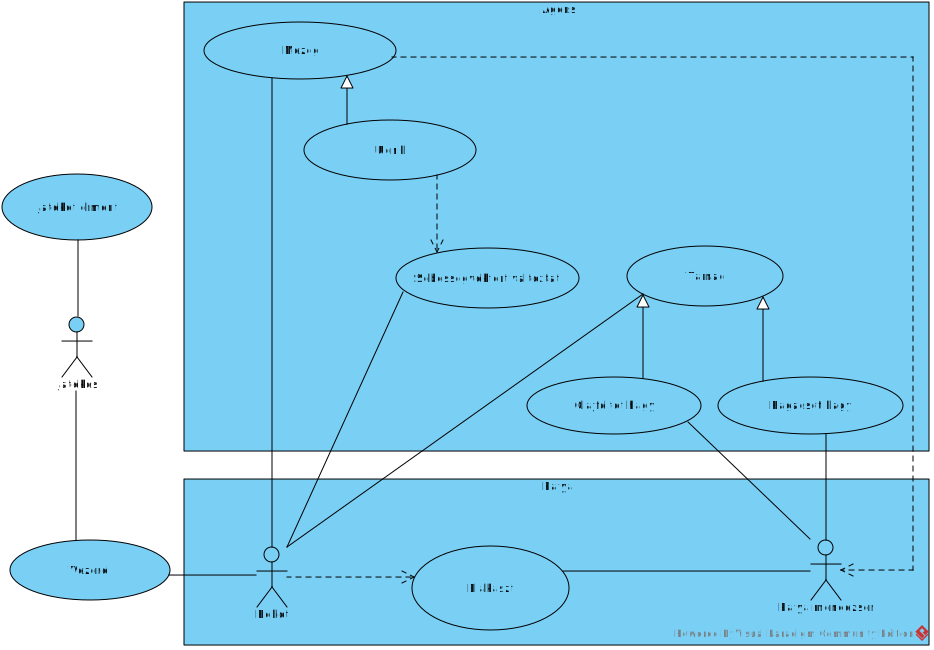
\includegraphics[width=\textwidth]{./chapters/chapter02/importantUseCases.pdf}

\subsection{Use-case leírások}
%\comment{Minden use-case-hez külön}

\usecase{Vezérel}%
{Játékos ezen a módon tudja irányítani a Robotot a pályán}%
{Játékos; Robot}%
{Játékos a helyzet alapján dönt arról, hogy a Robotnak mit kéne lépnie és utasítani fogja arra, hogy ezt tegye is meg}

\usecase{Játékot elment}%
{Így elmenthetjük a játék állapotát későbbi továbbjátszás céljából}%
{Játékos}%
{A Játékosnak játék közben más dolga akad azonban később szeretné folytatni a már elkezdettt játékát ezért elmentheti annak az állását}

\usecase{Mozog}%
{A Robot mozoghat a pályán. A mozgásnak magának több módja is van}
{Robot}
{A Játékos irányítja a Robotot annak érdekében, hogy közelebb kerülhessen a célhoz. Ehhez természetesen mozognia kell}

\usecase{Ugrik}%
{Mozgás egy fajtája, amely a sebességgel arányos lépést tesz}%
{-}%
{A Játékos a Robotot a cél felé irányítása folyamán ugrásra utasítja}

\usecase{Sebességvektort változtat}%
{A Robot megváltoztathatja a sebességvektorát}%
{Robot}%
{A Játékos a Robot cél fele való vezérélésének folytán megváltoztathatja a sebesség irányát és nagyságát is, például a pályán lévő kanyar bevételének céjából}

\usecase{Támad}%
{A Robot valamiképpen támadást végezhet a pályán}%
{Robot}%
{Ilyen támadásokkal más Robotokat hátráltathat valamilyen módon a továbbhaladásban}

\usecase{Olajfoltot hagy}%
{Egy Támadás fajta}%
{Pálya menedzser}%
{Robotok egymás hátráltatására olajfoltot hagyhatnak a pályán, mely ezután akadályozza a további Robotokat a sebesség megváltoztatásában}

\usecase{Ragacsot hagy}%
{Egy Támadás fajta}%
{Pálya menedzser}%
{Robotok egymás hátráltatására ragacsfoltot hagyhatnak a pályán, mely ezután megfelezi a többi Robotnak a sebességvektorát}

\usecase{Elakaszt}%
{Robotok szabálybetartásának végrehajtása}%
{Pálya menedzser}%
{Egy olyan Robot meg megsértette a játék szabályait valamely módon például lemegy a pálya határairól, azt a Pálya menedzser elakaszhatja ezáltal kizárva a játékból}

\section{Szótár}

\begin{tabularx}{\textwidth}{| l | l |}
\hline
\textbf{Bejegyzés} & \textbf{Definíció} \tabularnewline 
\hline\hline
    ágens & a robot maga \tabularnewline \hline
    ágensleíró &  az állapotot meghatározó változó, melyből több is lehet, ezeket a telepes változtathatja \tabularnewline \hline
    áll &  robot kezdeti állapota, jelenlegi helyzetben a sebességvektor 0 mértékű \tabularnewline \hline
    állapot &  a robot leírója, mely meghatározza az érvényes cselekvéseinek halmazát \tabularnewline \hline
    buff &  olyan hatás, mely pozitív vagy negatív módon járulhat hozzá a robot játékához \tabularnewline \hline
    birtokol & a robot tárolójában készlet van belőle \tabularnewline \hline
    célfüggvény & a győzelemhez ennek maximalizálása szükséges, a pontszám növelése  \tabularnewline \hline
    curse (átok) & olyan buff melynek a robotra negatív hatása van, csökkenti a nyerési esélyeit \tabularnewline \hline
    entitás &  egy szereplő a játékban \tabularnewline \hline 
    esemény & valamely történés, melyet egy játékos cselekvése váltott ki \tabularnewline \hline
    folt &  a mezőn helyezkedik el, buffot válthat ki \tabularnewline \hline
    grid (négyzetrács) & a pálya felosztása, jelenleg négyzetesen \tabularnewline \hline
    győztes &  jelenleg a leghosszabb utat megtett robot \tabularnewline \hline
    használ &  a készlet egy elemét aktiválja, mely kiváltja az általa definiált buffot \tabularnewline \hline
    határ &  a pálya tulajdonsága, melyen túl nincsenek mezők \tabularnewline \hline
    idő &  a verseny időtartama \tabularnewline \hline
    irányít &  a folyamat melynek során a telepes a robot ágensleíróit módosíthatja \tabularnewline \hline
    játékos &  a telepest irányító entitás \tabularnewline \hline
    készlet &  egy adott tárgy leírására alkalmas, mennyiséggel rendelkezik, a robot használhatja \tabularnewline \hline
    kiesik &  a robot elhagyja a pályát \tabularnewline \hline
    kivált &  esemény, melynek során valamely entitásra hat a kiváltó objektum \tabularnewline \hline
    mező &  objektum vagy objektumok tárolására alkalmas egység, lehet szabad és foglalt \tabularnewline \hline
    mozog &  a robot pozícióját megváltoztató vezérlés \tabularnewline \hline
    nyerési feltételek &  azon feltételek, melyeket egy robot teljesítve győztesnek tekinthető \tabularnewline \hline
    objektum &  jelenleg robot, folt \tabularnewline \hline
    olajfolt &  egy folt, mely kivált egy buffot, ami nem engedi a sebességvektor megváltoztatását \tabularnewline \hline
    olajkészlet &  egy készlet, mely az olajfolttal egyező buffot vált ki \tabularnewline \hline
    pálya &  a játéktér, mely mezőkből áll \tabularnewline \hline
    perk (áldás) & olyan buff melynek a robotra pozitív hatása van, növeli a nyerési esélyeket  \tabularnewline \hline
    pontszám &  a győztes meghatározásához szükséges mérték, a megtett útban \tabularnewline \hline
    pozíció &  a robot helyzete a pályán \tabularnewline \hline
    ragacsfolt &  egy folt, mely kivált egy buffot, ami megfelezi a sebességvektort \tabularnewline \hline
    ragacskészlet &  egy készlet, mely a ragacsfolttal egyező buffot vált ki \tabularnewline \hline
    robot &  a pályán elhelyezkedő, mezőn álló entitás, melyet a telepes irányít \tabularnewline \hline
    sebesség &  a robot mozgását meghatározó mérték, megmondja a robot hány mezőt léphet \tabularnewline \hline
    sebességvektor &  egy ágensleíró, mely meghatározza a sebességet \tabularnewline \hline
    tárgy & jelenleg olaj vagy ragacs   \tabularnewline \hline
    tároló &  benne találhatóak a készletek \tabularnewline \hline
    telepes &  a robotot irányító entitás \tabularnewline \hline
    ugrik &  jelenleg a mozgás egyetlen módja, mezőről-mezőre mozgatás \tabularnewline \hline
    verseny &  a játék menete, melyben nyerési feltételek vannak definiálva \tabularnewline \hline
    vezérel & lsd. irányít \tabularnewline \hline
\end{tabularx}

\section{Projekt terv}
\subsection{Csapatfelépítés}
A csapat négy főből áll. A szerepköröket a projekt elején kiosztottuk, figyelembe véve az egyes csapattagok preferenciáit. A cél az volt, hogy mindenki olyan feledatot kapjon, amely egybeesik a szakterületével.

\begin{tabularx}{\textwidth}{| l | l |}
\hline
\textbf{Név} & \textbf{Szerepkör} \tabularnewline 
\hline\hline
Nagy Gergő (csapatvezető) & kód, management, dokumentáció \tabularnewline \hline
Nyári Dávid Tamás & kód, UML, dokumentáció \tabularnewline \hline
Paral Zsolt & kód, grafika, dokumentáció \tabularnewline \hline
Szőke-N István & grafika, UML, dokumentáció \tabularnewline \hline
\end{tabularx}

\subsection{Kommunikáció}
A csapat tagjai három fő módon kommunikálnak egymással:
\begin{enumerate}
    \item \textbf{Facebook:} egy privát Facebook csoport, amelyben elsősorban menedzsment jellegű megbeszélések folynak, mint például konferenciák időpontjainak egyesztetése, pull request review megsürgetése. Napi rendszerességű a kommunikáció.
    \item \textbf{Google Hangouts:} a konferenciák lebonyolításának elsődleges formája. A legfontosabb közös döntések, feladatkiosztások itt történnek. Rendszeressége függ a megvitatandó problémák számától: a projekt elején akár heti 2-3 alkalom is előfordulhat, de a későbbiekben jellemzően heti rendszerességű lesz.
    \item \textbf{GitHub:} minden egyéb kommunikáció a GitHubon zajlik. Fontosabb általános tudnivalók a \textit{Wikin} találhatók, a konkrét problémákról való megbeszélések az \textit{Issues} menü alatt, míg mások kódjának ellenőrzése a \textit{Pull Request} menü alatt található. A kommunikáció gyakorisága függ a kontribúciók rendszerességétől és a felmerülő problémák számától, de ennek a módnak a legfőbb feladata, hogy a projekthez kapcsolódó problémák egy centralizált helyen legyenek
        megbeszélve és dokumentálva.
\end{enumerate}

\subsection{Verziókezelés, fejlesztés}
Mivel többen dolgozunk egyszerre a projekten, ezért fontos, hogy mindenki hozzá tudjon férni a legfrissebb forráskódhoz és dokumentációhoz. Ezen felül elsődleges szempont, hogy a párhuzamosan dolgozó csapataggok munkája könnyen integrálható legyen a közponi (beadandó) kózbázisba. \\ 
Ehhez mi a \textbf{Git} verziókezelő rendszert, központi tárhelynek pedig a \textbf{GitHubot}  használjuk, különböző kiegészítésekkel. Ez lehetőséget biztosít a kód könnyű nyomonkövetésére, illetve
esetleges hibák esetén egy korábbi változatra való visszaállásra (bár ezt mindenáron el akarjuk kerülni, ld. a következő pontokat). Mivel a dokumentáció elkészítéséhez a LaTeX rendszert választottuk, ezért a dokumentáció is egyszerűen kezelhető a verziókezelőben. \\
Kiegészítések a Git és GitHub beépített eszközeihez:

\begin{enumerate}
    \item \textbf{Waffle.io:} központi felületet biztosít a projekthez tartozó \textit{Issuek} kezeléséhez, az értük felelős csapattagok nyílvántartásához
    \item \textbf{TravisCI:} a projekt folyamatos integrációt használ, amellyel több probléma is elkerülhető:
        \begin{itemize}
            \item Mivel a TravisCI-n a laborban található gépekkel egyező verziójú Java fut, ezért a kódban biztos nem találhatók nem megfelelő szabványból származó elemek. 
            \item Biztosított, hogy a kód szintaktikai hibákat nem tartalmaz, hiszen a kódnak le kell fordulnia a build serveren. 
            \item Garantált hogy átment az összes, a projektben definiált unit testen. 
        \end{itemize} 
        Ez a folyamatos integrációs folyamat minden egyes elküldött \textit{Pull Requestre} lefut, így biztosan nem kerül a fő ágba olyan kód, amely a fent említett három probléma bármelyikét tartalmazza.
    \item \textbf{Coverity:} egy statikus ellenőrzést végző alkalmazás. Fontosabb mérföldkövek után kerül futtatásra. Feladata, hogy segítsen rejtett hibák feltárásában és kijavításában.
\end{enumerate}


\subsection{Egyéb programok}
A fent kifejtett módszer mellett a csapat tagjai az alábbi programokat használják a fejlesztéshez: \\ 

\noindent \textbf{Dokumentáció:} TeXStudio vagy egyszerű szövegszerkesztő program (Vim, GEdit). \\

\noindent \textbf{UML:} a könnyű együttműködés érdekében a csapat összes tagja ugyanazt az UML IDE-t használja, ez pedig a Visual Paradigm Community Edition \\

\noindent \textbf{Java:} nincs meghatározott fejlesztőkörnyezet, a használt programok listája: IntelliJ IDEA, Eclipse, Vim

\subsection{Határidők}

\begin{tabularx}{\linewidth}{| l | l | l |}
\hline
\textbf{Dátum} & \textbf{Leírás} & \textbf{Ellenőrzés} \tabularnewline 
\hline \hline
\endhead
2015. 02. 23. & Követelmény, projekt, funkcionalitás & beadás \tabularnewline \hline
2015. 03. 02. & Analízis modell kidolgozása 1. & beadás \tabularnewline \hline
2015. 03. 09. & Analízis modell kidolgozása 2. & beadás \tabularnewline \hline
2015. 03. 16. & Szkeleton tervezése & beadás \tabularnewline \hline
2015. 03. 23. & Szkeleton beadás & beadás \tabularnewline \hline
2015. 03. 25. & \textbf{Szkeleton} & bemutatás \tabularnewline \hline
2015. 03. 30. & Prototípus koncepciója & beadás \tabularnewline \hline
2015. 04. 07. & Részletes tervek & beadás \tabularnewline \hline
2015. 04. 20. & Prototípus & beadás \tabularnewline \hline
2015. 04. 22. & \textbf{Prototípus} & bemutatás \tabularnewline \hline
2015. 04. 27. & Grafikus felület specifikációja & beadás \tabularnewline \hline
2015. 05. 11. & Grafikus változat & beadás \tabularnewline \hline
2015. 05. 13. & \textbf{Grafikus változat} & bemutatás \tabularnewline \hline
2015. 05. 15. & Összefoglalás & beadás \tabularnewline \hline
\end{tabularx}

\subsection{Mérföldkövek}
A feladatot három fő lépcsöben kell megvalósítani:
\begin{enumerate}
    \item szkeleton
    \item prototípus
    \item grafikus
\end{enumerate}

\noindent A \textbf{szkeleton} változat célja annak bizonyítása, hogy az objektum és dinamikus modellek a definiált feladat egy modelljét alkotják. A szkeleton egy program, amelyben már valamennyi, a végső rendszerben is szereplő business objektum szerepel. Az objektumoknak csak az interfésze definiált. Valamennyi metódus az indulás pillanatában az ernyőre szöveges változatban kiírja a saját nevét, majd meghívja azon metódusokat, amelyeket a szolgáltatás végrehajtása érdekében meg kell hívnia. Amennyiben
a metódusból valamely feltétel fennállása esetén hívunk meg más metódusokat, akkor a feltételre vonatkozó kérdést interaktívan az ernyőn fel kell tenni és a kapott válasz alapján kell a továbbiakban eljárni. A szkeletonnak alkalmasnak kell lenni arra, hogy a különböző forgatókönyvek és szekvencia diagramok ellenőrizhetők legyenek. Csak karakteres ernyőkezelés fogadható el, mert ez biztosítja a rendszer egyszerűségét. \\ 

\noindent A \textbf{prototípus} program célja annak demonstrálása, hogy a program elkészült, helyesen működik, valamennyi feladatát teljesíti. A prototípus változat egy elkészült program kivéve a kifejlett grafikus interfészt. A változat tervezési szempontból elkészült, az ütemezés, az aktív objektumok kezelése megoldott. A business objektumok - a megjelenítésre vonatkozó részeket kivéve - valamennyi metódusa a végleges algoritmusokat tartalmazza. A megjelenítés és működtetés egy alfanumerikus ernyőn
követhető, ugyanakkor a megjelenítés fájlban is logolható, ezzel megteremtve a rendszer tesztelésének lehetőségét. Különös figyelmet kell fordítani az interfész logikájára, felépítésére, valamint arra, hogy az mennyiben tükrözi és teszi láthatóvá a program működését, a beavatkozások hatásait. \\

\noindent A teljes (\textbf{grafikus}) változat a prototípustól elvileg csak a kezelői felület minőségében különbözhet. Ennek változatnak az értékelésekor a hangsúlyt sokkal inkább a megvalósítás belső szerkezetére, semmint a külalakra kell helyezni.

% Szglab4
% ===========================================================================
%
\section{Napló}

\begin{naplo}

\bejegyzes
{2015.02.15 ~19.00}
{1 óra}
{Paral \newline Nagy} 
{Értekezlet.
Döntés: Paral előkészíti a coverage eszközt és az automata tesztelést. \newline
Nagy előkészíti a Travis CI-t és a LaTeX build scriptet.} 

\bejegyzes
{2015.02.16 ~19.00}
{1 óra}
{Paral \newline Nyári \newline Szőke \newline Nagy} 
{Értekezlet.
Döntés: Feladatok felosztása az feladatok hozzárendelése a megfelelő emberekhez. \newline } 

\bejegyzes
{2015.02.18. ~19.00}
{1 óra}
{Paral \newline Nyári \newline Szőke \newline Nagy} 
{Értekezlet.
Döntés: Feladatok előrehaladásának ellenőrzése, kritikus kérdések átbeszélése. \newline } 

\bejegyzes
{2015.02.20. ~19.00}
{1 óra}
{Paral \newline Nyári \newline Szőke \newline Nagy} 
{Értekezlet.
Döntés: Feladatok tisztázása, kész feladatok mergelése. Utolsó simítások átbeszélése. \newline } 

\bejegyzes
{2015.02.17. ~21.00}
{0.5 óra}
{Paral} 
{Tevékenység: Elkészíti a Szakterület szekciót.\newline } 

\bejegyzes
{2015.02.20. ~19.30}
{2 óra}
{Paral} 
{Tevékenység: Elkészíti a Projektterv szekciót.\newline } 

\bejegyzes
{2015.02.20. ~21.30}
{1 óra}
{Paral} 
{Tevékenység: Elkészíti az Átadással kapcsolat követelmények szekciót.\newline } 

\bejegyzes
{2015.02.19. ~19.00}
{30 perc}
{Paral} 
{Tevékenység: Elkészíti a Erőforrásokkal kapcsolatos szekciót.\newline } 

\bejegyzes
{2015.02.18. ~17.00}
{15 perc}
{Paral} 
{Tevékenység: Elkészíti a Feltételezések, kapcsolatok szekciót.\newline } 

\bejegyzes
{2015.02.17. ~20.00}
{3 óra}
{Nyári} 
{Tevékenység: Elkészíti a Lényeges use-casek szekciót.\newline } 

\bejegyzes
{2015.02.18. ~8.00}
{2 óra}
{Nyári} 
{Tevékenység: Elkészíti a Konzultációs jegyzőkönyvet.\newline } 

\bejegyzes
{2015.02.18. ~18.00}
{1 óra}
{Nyári} 
{Tevékenység: Elkészíti az Általános áttekintést.\newline } 

\bejegyzes
{2015.02.21. ~18.00}
{1.5 óra}
{Nyári} 
{Tevékenység: Elkészíti a Funkcionális követelmények szekciót.\newline } 

\bejegyzes
{2015.02.18. ~18.00}
{3 óra}
{Szőke} 
{Tevékenység: Elkészíti a Nem funkcionális követelmények szekciót.\newline } 

\bejegyzes
{2015.02.18. ~21.00}
{30 perc}
{Szőke} 
{Tevékenység: Elkészíti a Korlátozások szekciót.\newline } 

\bejegyzes
{2015.02.19. ~18.00}
{30 perc}
{Szőke} 
{Tevékenység: Elkészíti a Felhasználók szekciót.\newline } 

\bejegyzes
{2015.02.19. ~18.00}
{15 perc}
{Nagy} 
{Tevékenység: Elkészíti a Hivatkozások szekciót.\newline } 

\bejegyzes
{2015.02.19. ~18.30}
{15 perc}
{Nagy} 
{Tevékenység: Elkészíti az Összefoglalás szekciót.\newline } 

\bejegyzes
{2015.02.21. ~23.00}
{3 óra}
{Nagy} 
{Tevékenység: Elkészíti az Funkciók szekciót.\newline } 

\bejegyzes
{2015.02.20 ~23.00}
{15 perc}
{Nagy} 
{Tevékenység: Elkészíti az Cél megfogalmazása szekciót.\newline } 

\bejegyzes
{Hét folyamán}
{1 óra}
{Paral} 
{Tevékenység: Reviewra szánt idő a pull-requestekre.\newline } 

\bejegyzes
{Hét folyamán}
{1 óra}
{Nyári} 
{Tevékenység: Reviewra szánt idő a pull-requestekre.\newline } 

\bejegyzes
{Hét folyamán}
{2 óra}
{Szőke} 
{Tevékenység: Reviewra szánt idő a pull-requestekre.\newline } 

\bejegyzes
{Hét folyamán}
{2 óra}
{Nagy} 
{Tevékenység: Reviewra szánt idő a pull-requestekre.\newline } 

\bejegyzes
{2015.02.13}
{1 óra}
{Paral \newline Nagy} 
{Értekezlet: Felveszik az feladatokat.\newline } 


\end{naplo}



%\setcounter{chapter}{2}
%% Szglab4
% ===========================================================================
%
\chapter{Analízis modell kidolgozása 1}

\thispagestyle{fancy}

\section{Objektum katalógus}

\comment{Minden, a feladatban szereplő objektum rövid, egy-két bekezdés hosszú ismertetése. Meg kell jelenjen minden objektumhoz, hogy mi a felelőssége. Informális leírás, ezért nem kell foglalkozni az örökléssel, az interfészekkel, az absztrakt osztályokkal, a segédosztályokkal.}

\subsection{Objektum1}
\comment{Felelősség informális leírása}

\subsection{Objektum2}
\comment{Felelősség informális leírása}

\section{Statikus struktúra diagramok}
\comment{Az előző alfejezet osztályainak kapcsolatait és publikus metódusait bemutató osztálydiagram(ok). Tipikus hibalehetőségek: csillag-topológia, szigetek.}

\begin{figure}[h]
\begin{center}
%\includegraphics[width=17cm]{chapters/chapter03/example.pdf}
\caption{x}
\label{fig:example1}
\end{center}
\end{figure}


\section{Osztályok leírása}
\comment{Az előző alfejezetben tárgyalt objektumok felelősségének formalizálása attribútumokká, metódusokká. Csak publikus metódusok szerepelhetnek. Ebben az alfejezetben megjelennek az interfészek, az öröklés, az absztrakt osztályok. Segédosztályokra még mindig nincs szükség. Az osztályok ABC sorrendben kövessék egymást. Interfészek esetén az Interfészek, Attribútumok pontok kimaradnak.}

\subsection{Osztály1}
\begin{itemize}
\item Felelősség\\
\comment{Mi az osztály felelőssége. Kb 1 bekezdés.}
\item Ősosztályok\\
\comment{Mely osztályokból származik (öröklési hierarchia)\newline
Legősebb osztály $\rightarrow$ Ősosztály2 $\rightarrow$ Ősosztály3...}
\item Interfészek\\
\comment{Mely interfészeket valósítja meg.}
\item Attribútumok\\
\comment{Milyen attribútumai vannak}
	\begin{itemize}
		\item attribútum1: attribútum jellemzése: mire való
		\item attribútum2: attribútum jellemzése: mire való
	\end{itemize}
\item Metódusok\\
\comment{Milyen publikus metódusokkal rendelkezik. Metódusonként egy-három mondat arról, hogy a metódus mit csinál.}
	\begin{itemize}
		\item int foo(Osztály3 o1, Osztály4 o2): metódus leírása
		\item int bar(Osztály5 o1): metódus leírása
	\end{itemize}
\end{itemize}

\subsection{Osztály2}
\begin{itemize}
\item Felelősség\\
\comment{Mi az osztály felelőssége. Kb 1 bekezdés.}
\item Ősosztályok\\
\comment{Mely osztályokból származik (öröklési hierarchia)\newline
Legősebb osztály $\rightarrow$ Ősosztály2 $\rightarrow$ Ősosztály3...}
\item Interfészek\\
\comment{Mely interfészeket valósítja meg.}
\item Attribútumok\\
\comment{Milyen attribútumai vannak}
	\begin{itemize}
		\item attribútum1: attribútum jellemzése: mire való
		\item attribútum2: attribútum jellemzése: mire való
	\end{itemize}
\item Metódusok\\
\comment{Milyen publikus metódusokkal rendelkezik. Metódusonként egy-három mondat arról, hogy a metódus mit csinál.}
	\begin{itemize}
		\item int foo(Osztály3 o1, Osztály4 o2): metódus leírása
		\item int bar(Osztály5 o1): metódus leírása
	\end{itemize}
\end{itemize}

\section{Statikus struktúra diagramok}
\comment{Az előző alfejezet osztályainak kapcsolatait és publikus metódusait bemutató osztálydiagram(ok). Tipikus hibalehetőségek: csillag-topológia, szigetek.}

\begin{figure}[h]
\begin{center}
%\includegraphics[width=17cm]{chapters/chapter03/example.pdf}
\caption{x}
\label{fig:example1}
\end{center}
\end{figure}

\section{Szekvencia diagramok}
\comment{Inicializálásra, use-case-ekre, belső működésre. Konzisztens kell legyen az előző alfejezettel. Minden metódus, ami ott szerepel, fel kell tűnjön valamelyik szekvenciában. Minden metódusnak, ami szekvenciában szerepel, szereplnie kell a valamelyik osztálydiagramon.}

\begin{figure}[h]
	\begin{center}
		\includegraphics[width=\textwidth]{chapters/chapter03/agentsRobotacceptAgentCommand.pdf}
		\caption{Robot utasítást fogad}
		\label{fig:agents.Robot.accept}
	\end{center}
\end{figure}

\begin{figure}[h]
	\begin{center}
		\includegraphics[width=\textwidth]{chapters/chapter03/agentsRobotaddOil.pdf}
		\caption{Robot felvesz a készletébe egy olajfoltot}
		\label{fig:agents.Robot.accept}
	\end{center}
\end{figure}

\begin{figure}[h]
	\begin{center}
		\includegraphics[width=\textwidth]{chapters/chapter03/agentsRobotaddSticky.pdf}
		\caption{Robot felvesz a készletébe egy ragacsfoltot}
		\label{fig:agents.Robot.accept}
	\end{center}
\end{figure}

\section{State-chartok}
\comment{Csak azokhoz az osztályokhoz, ahol van értelme. Egyetlen állapotból álló state-chartok ne szerepeljenek. A játék működését bemutató state-chart-ot készíteni tilos.}

\begin{figure}[h]
\begin{center}
%\includegraphics[width=17cm]{chapters/chapter03/example.pdf}
\caption{x}
\label{fig:example3}
\end{center}
\end{figure}


%% Szglab4
% ===========================================================================
%
\section{Napló}

\begin{naplo}

\bejegyzes
{2015.02.25. ~8.00}
{2 óra}
{Nagy} 
{Tevékenység: Elkészíti a Konzultációs jegyzőkönyvet.\newline } 

\bejegyzes
{2015.02.15 ~19.00}
{1 óra}
{Nagy} 
{Nagy előkészíti a feladatokat, felveszi őket a GitHub-ra..} 

\bejegyzes
{2015.02.25 ~20.00}
{2 óra}
{Paral \newline Nyári \newline Szőke \newline Nagy} 
{Értekezlet.
Döntés: Feladatok felosztása az feladatok hozzárendelése a megfelelő emberekhez. A részletek megbeszélése, tervezés, koncepciók átgondolása.\newline } 

\bejegyzes
{2015.02.26. ~20.00}
{1 óra}
{Paral \newline Nyári \newline Szőke \newline Nagy} 
{Értekezlet.
Döntés: Általános megbeszélés, előrehaladás ellenőrzése. A felmerülő problémák azonosítása és eliminálása. \newline } 

\bejegyzes
{2015.02.27. ~19.00}
{2 óra}
{Paral \newline Nyári \newline Szőke \newline Nagy} 
{Értekezlet.
Döntés: Elkészült tervek átnézése, lehetséges jövőbeli problémák azonosítása az architektúrával kapcsolatban. Hátralévő feladatok azonosítása.\newline } 

\bejegyzes
{2015.02.27. ~21.00}
{1 óra}
{Paral \newline Nyári \newline Szőke \newline Nagy} 
{Értekezlet.
Döntés: Elkészült tervek utolsó átnézése, apróbb módosítások kiosztása.\newline } 

\bejegyzes
{2015.02.26. ~17.00}
{5 óra}
{Paral} 
{Tevékenység: Statikus struktúra diagrammok szekció elkészítése.\newline } 

\bejegyzes
{2015.02.27. ~8.00}
{2 óra}
{Nyári} 
{Tevékenység: Statikus struktúra diagrammok szekcióban apróbb módosítások eszközölése.\newline } 

\bejegyzes
{2015.02.27. ~13.00}
{2 óra}
{Szőke} 
{Tevékenység: Statikus struktúra diagrammok szekcióban apróbb módosítások eszközölése.\newline } 

\bejegyzes
{2015.02.25. ~21.00}
{2 óra}
{Paral} 
{Tevékenység: Objektumkatalógus szekció elkészítése.\newline } 

\bejegyzes
{2015.02.25. ~21.00}
{5 óra}
{Nyári} 
{Tevékenység: Szekvenciadiagrammok szekció elkészítése.\newline } 

\bejegyzes
{2015.02.26. ~15.00}
{2 óra}
{Szőke} 
{Tevékenység: További szekvenciadiagrammok szekció elkészítése.\newline } 

\bejegyzes
{2015. 02.28. ~10.00}
{1 óra}
{Nagy}
{Tevékenység: Osztályleírások elkészítése.\newline }

\bejegyzes
{2015.02.28. ~12.00}
{1 óra}
{Paral}
{Tevékenység: Osztályleírások átnézése, finomítása.\newline}

\bejegyzes
{2015.02.28. ~16.00}
{30 perc}
{Nyári}
{Tevékenység:  State Chart diagramok elkészítése}

\bejegyzes
{2015.02.28 ~17.00}
{1 óra}
{Paral} 
{Tevékenység: Reviewra szánt idő a pull-requestekre.\newline } 

\bejegyzes
{2015.02.28. ~17.00}
{1 óra}
{Nyári} 
{Tevékenység: Reviewra szánt idő a pull-requestekre.\newline } 

\bejegyzes
{2015.02.28. ~17.00}
{1 óra}
{Szőke} 
{Tevékenység: Reviewra szánt idő a pull-requestekre.\newline } 

\bejegyzes
{2015.02.28. ~17.00}
{1 óra}
{Nagy} 
{Tevékenység: Reviewra szánt idő a pull-requestekre.\newline } 

\bejegyzes
{2015.03.1. ~8.00}
{1 óra}
{Nagy} 
{Tevékenység: Követelmények, projekt, funckionalitás leadandó módosításainak hozzáadása.\newline } 

\bejegyzes
{2015.03.1. ~10.00}
{1 óra}
{Nagy} 
{Tevékenység: Napló elkészítése.\newline } 

\end{naplo}



%\setcounter{chapter}{3}
%% Szglab4
% ===========================================================================
%
\chapter{Analízis modell kidolgozása 2}

\thispagestyle{fancy}

\section{Objektum katalógus}

\subsection{Command}
\begin{tabularx}{\linewidth}{| l | X |}
\hline
\textbf{Név} & \textbf{Leírás} \tabularnewline
\hline\hline
\endhead
ChangeDirectionQuery & Egy robottól irányváltoztatást kérő parancs. Elő tudja állítani a megfelelő \textbf{ChangeDirectionTransmit} parancsot. \tabularnewline\hline

ChangeDirectionTransmit & Az az irányváltoztató parancs, amit egy cella módosítani tud a rajta található buffokkal. Elő tudja állítani a megfelelő \textbf{ChangeDirectionExecute} parancsot. \tabularnewline\hline 

ChangeDirectionExecute & Az ugrást a \textbf{Roboton} ténylegesen végrehajtó parancs. \tabularnewline\hline

ChangeSpeedQuery & Egy robottól sebességváltoztatást kérő parancs. Elő tudja állítani a megfelelő \textbf{ChangeSpeedTransmit} parancsot. \tabularnewline\hline

ChangeSpeedTransmit & Az a sebességváltoztató parancs, amit egy cella módosítani tud a rajta található buffokkal. Elő tudja állítani a megfelelő \textbf{ChangeSpeedExecute} parancsot. \tabularnewline\hline

ChangeSpeedExecute & A sebességváltoztatást a \textbf{Roboton} ténylegesen végrehajtó parancs. \tabularnewline\hline

JumpQuery & Egy robottól ugrás kezdeményezését kérő parancs. Lekérdezi és tárolja a robot aktuális sebességét. Elő tudja állítani a megfelelő \textbf{JumpTransmit} parancsot.  \tabularnewline\hline

JumpTransmit & Az az ugróparancs, amit egy cella módosítani tud a rajta található buffokkal. Lekérdezi a cellától az ugrás kezdetét és célját, és tárolja ezeket. Elő tudja állítani a megfelelő \textbf{JumpExecute} parancsot. \tabularnewline\hline 

JumpExecute & Az ugrást a \textbf{Roboton}, a kezdő és cél cellán ténylegesen végrehajtó parancs. \tabularnewline\hline

KillExecute & Egy \textbf{Robotot} a játékból kiiktatni képes parancs. \tabularnewline\hline

TimoutExecute & Egy \textbf{Robotnak} jelzi, hogy elfogyott a rá kijelölt teljes időtartam. \tabularnewline\hline

UseOilQuery & Egy \textbf{Robotot} arra utasít, hogy helyezzen egy \textbf{Oil} buffot arra a mezőre, amelyen áll. Lekérdezi, hogy a robotnak van-e elérhető \textbf{Oil} készlete, és ezt tárolja. Elő tudja állítani a megfelelő \textbf{UseOilExecute} parancsot. \tabularnewline\hline

UseOilExecute & Egy \textbf{Oil} buffot helyez el a cellán. \tabularnewline\hline

UseStickyQuery & Egy \textbf{Robotot} arra utasít, hogy helyezzen egy \textbf{Sticky} buffot arra a mezőre, amelyen áll. Lekérdezi, hogy a robotnak van-e elérhető \textbf{Sticky} készlete, és ezt tárolja. Elő tudja állítani a megfelelő \textbf{UseStickyExecute} parancsot. \tabularnewline\hline

UseStickyExecute & Egy \textbf{Sticky} buffot helyez el a cellán. \tabularnewline\hline
\end{tabularx}

\subsection{Direction}
Tárolja egy \textbf{Robot} lehetséges mozgási irányait, és egyben a megfelelő \textbf{Cellek} lehetséges szomszédossági viszonyait.

\subsection{EmptyFieldCell}
Az \textbf{EmptyFieldCell} osztály példányai a pálya azon részeit tárolja, amelyre lépve a \textbf{Robotok} kiesnek a játékból. Az ő felelőssége a robotnak elküldeni azt a parancsot, ami ezt a hatást előidézi (\textbf{KillExecute}).
Tárolja a rajta álló robotot, illetve referenciákat a szomszédos mezőkre, amiket a megfelelő \textbf{Direction} megadásával érhetünk el. Tartalmazza ezen felül a céltól való távolságot, amelyet a nyertes meghatározására használhatunk. Az ő felelőssége annak a cellának a megkeresése, amelyre egy \textbf{Robot} ugorhat. A cellán átmenő parancsokat módosíthatja a rajta található buffokkal.

\subsection{FieldCell}
Ezen osztály példányai alkotják a pálya legnagyobb részét: minden olyan cella, amely nem a célvonal része, illetve nem a pálya szélét alkotja ilyen típusú. A \textbf{FieldCell} példányok fontos feldata, hogy a rálépő \textbf{Robotokon} érvényesítse a cellán lévő buffokat. Ezen felül a \textbf{Robotoknak} érkező parancsok egy része keresztülhalad ezeken a mezőkön, ahol a rajta található buffok ezeket a parancsokat módosíthatják. A \textbf{FieldCell} ezután a módosított parancsot
továbbítja a rajta álló \textbf{Robot} felé.
Tárolja a rajta álló robotot, illetve referenciákat a szomszédos mezőkre, amiket a megfelelő \textbf{Direction} megadásával érhetünk el. Tartalmazza ezen felül a céltól való távolságot, amelyet a nyertes meghatározására használhatunk. Az ő felelőssége annak a cellának a megkeresése, amelyre egy \textbf{Robot} ugorhat. A cellán átmenő parancsokat módosíthatja a rajta található buffokkal.

\subsection{FinishLineFieldCell}
A \textbf{FinishLineFieldCell} osztály példányainak felelősségei megegyeznek a \textbf{FieldCell} osztály példányainak felelősségeivel, azzal a különbséggel, hogy ezek a cellák jelzik egy körnek a végét.

\subsection{Inventory}
Buffok tárolására alkalmas, nyílvántartja a benne található buffok számát, és csak akkor engedi azokat használni, ha legalább egyet tartalmaz.

\subsection{Oil}
Egy olyan buff, aminek hatására a \textbf{Fieldre} lépő \textbf{Robotok} sebessége megfelelződik.

\subsection{Result}
Egy parancs lefutásának eredményét tárolja.

\subsection{Robot}
A \textbf{Robot} osztály példányai egy-egy pályán mozgó robotot tárolnak. Tárolja a saját sebességét, illetve azt a cellát, amin pillanatnyilag áll. Ezen felül rendelkeznek \textbf{Inventorykkal}, amelyben \textbf{Stickyt} vagy \textbf{Oilt} tárolnak. Ezeket le tudják helyezni arra a cellára, amelyen állnak.

\subsection{Speed}
Egy \textbf{Robot} sebességét reprezentálja.

\subsection{Sticky}
Egy olyan buff, ami képes a \textbf{JumpExecute} parancs olyan módosítására, amely megakadályozza azt, hogy ez a parancs megváltoztassa egy \textbf{Robot} sebességét.

\clearpage

\section{Statikus struktúra diagramok}

\begin{figure}[h]
	\begin{center}
		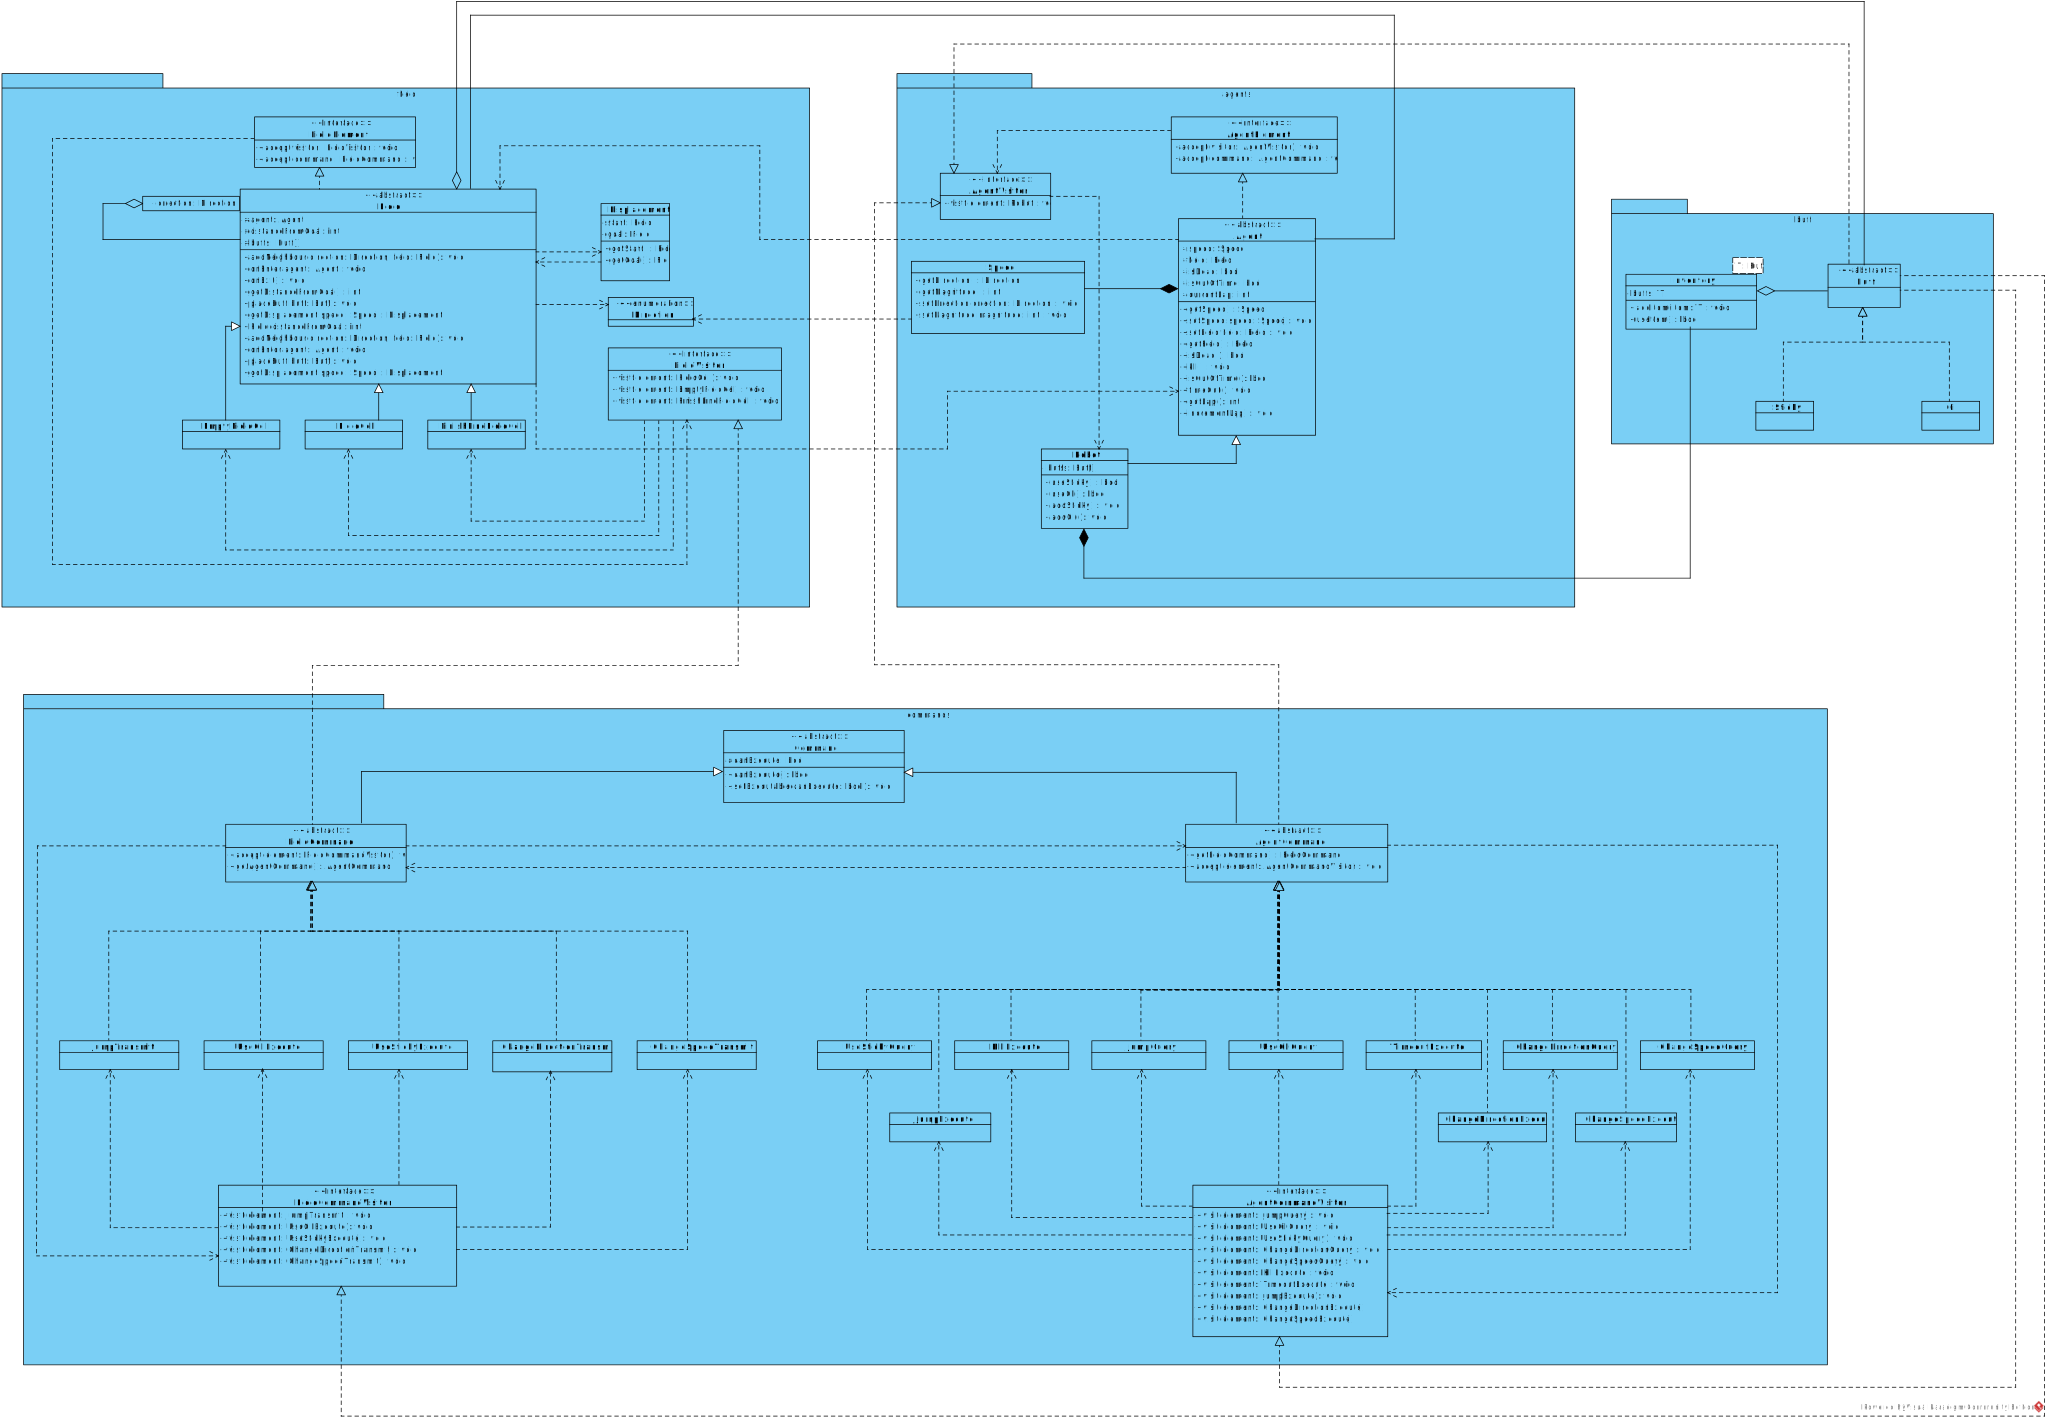
\includegraphics[width=\linewidth]{chapters/chapter04/ClassMain.pdf}
		\caption{A teljes osztálydiagram}
		\label{A teljes osztálydiagram}
	\end{center}
\end{figure}

\begin{figure}[h]
	\begin{center}
		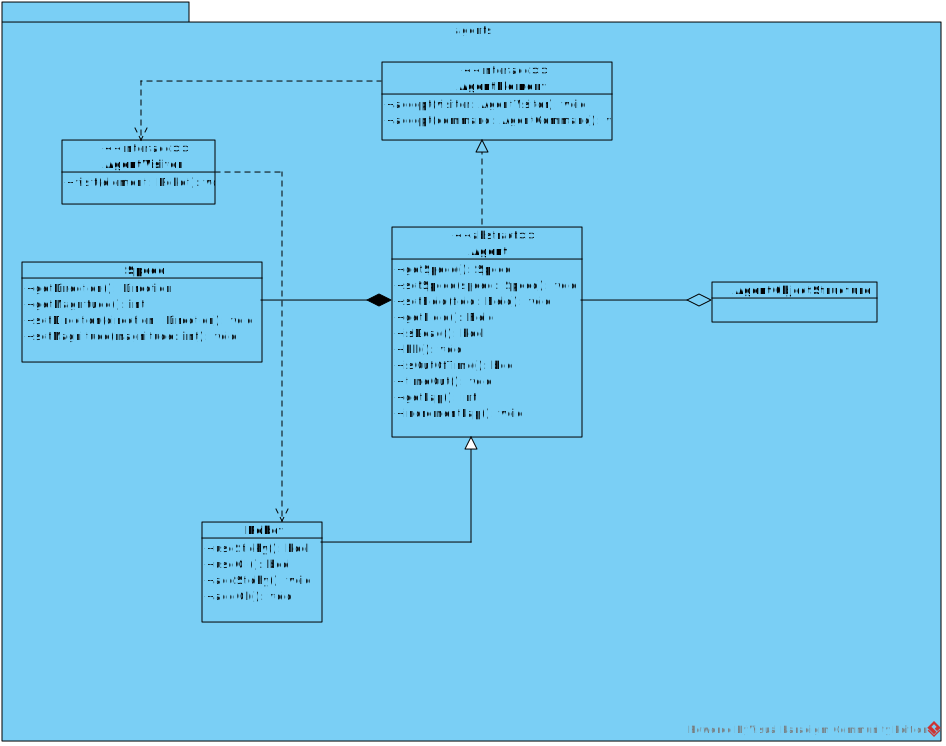
\includegraphics[width=\linewidth]{chapters/chapter04/ClassAgents.pdf}
		\caption{Agents package osztálydiagram}
		\label{Agents package osztálydiagram}
	\end{center}
\end{figure}

\begin{figure}[h]
	\begin{center}
		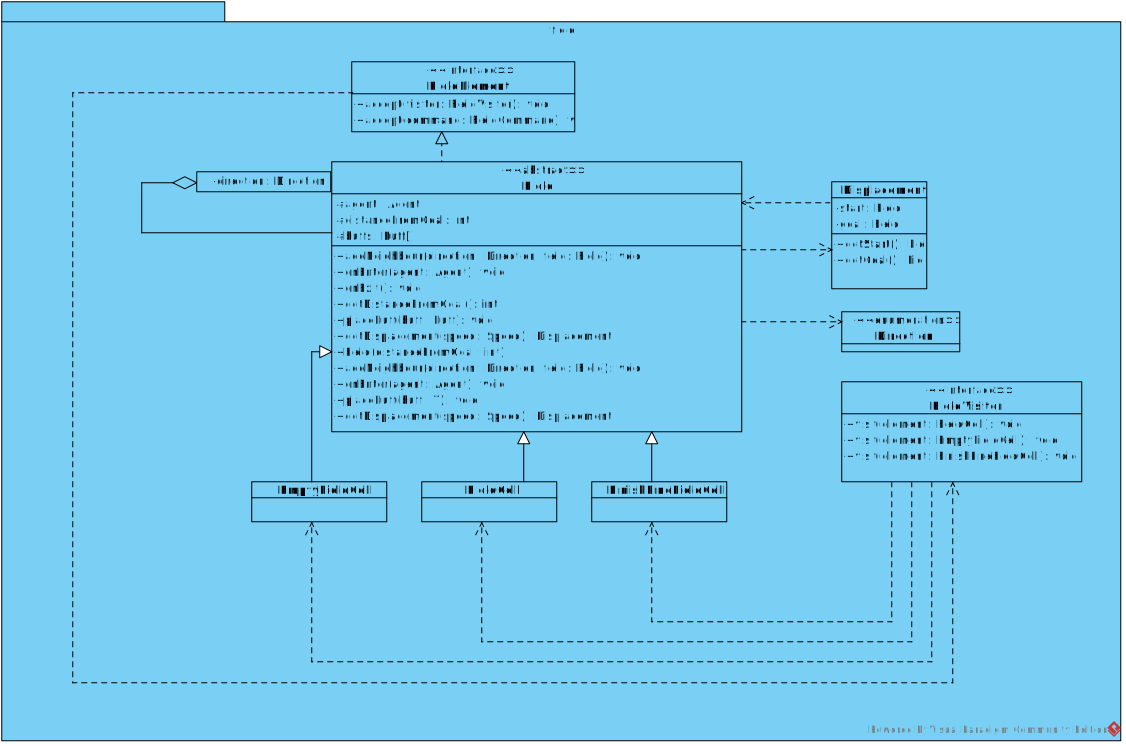
\includegraphics[width=\linewidth]{chapters/chapter04/ClassField.pdf}
		\caption{Field package osztálydiagram}
		\label{Field package osztálydiagram}
	\end{center}
\end{figure}

\clearpage

\begin{figure}[h]
	\begin{center}
		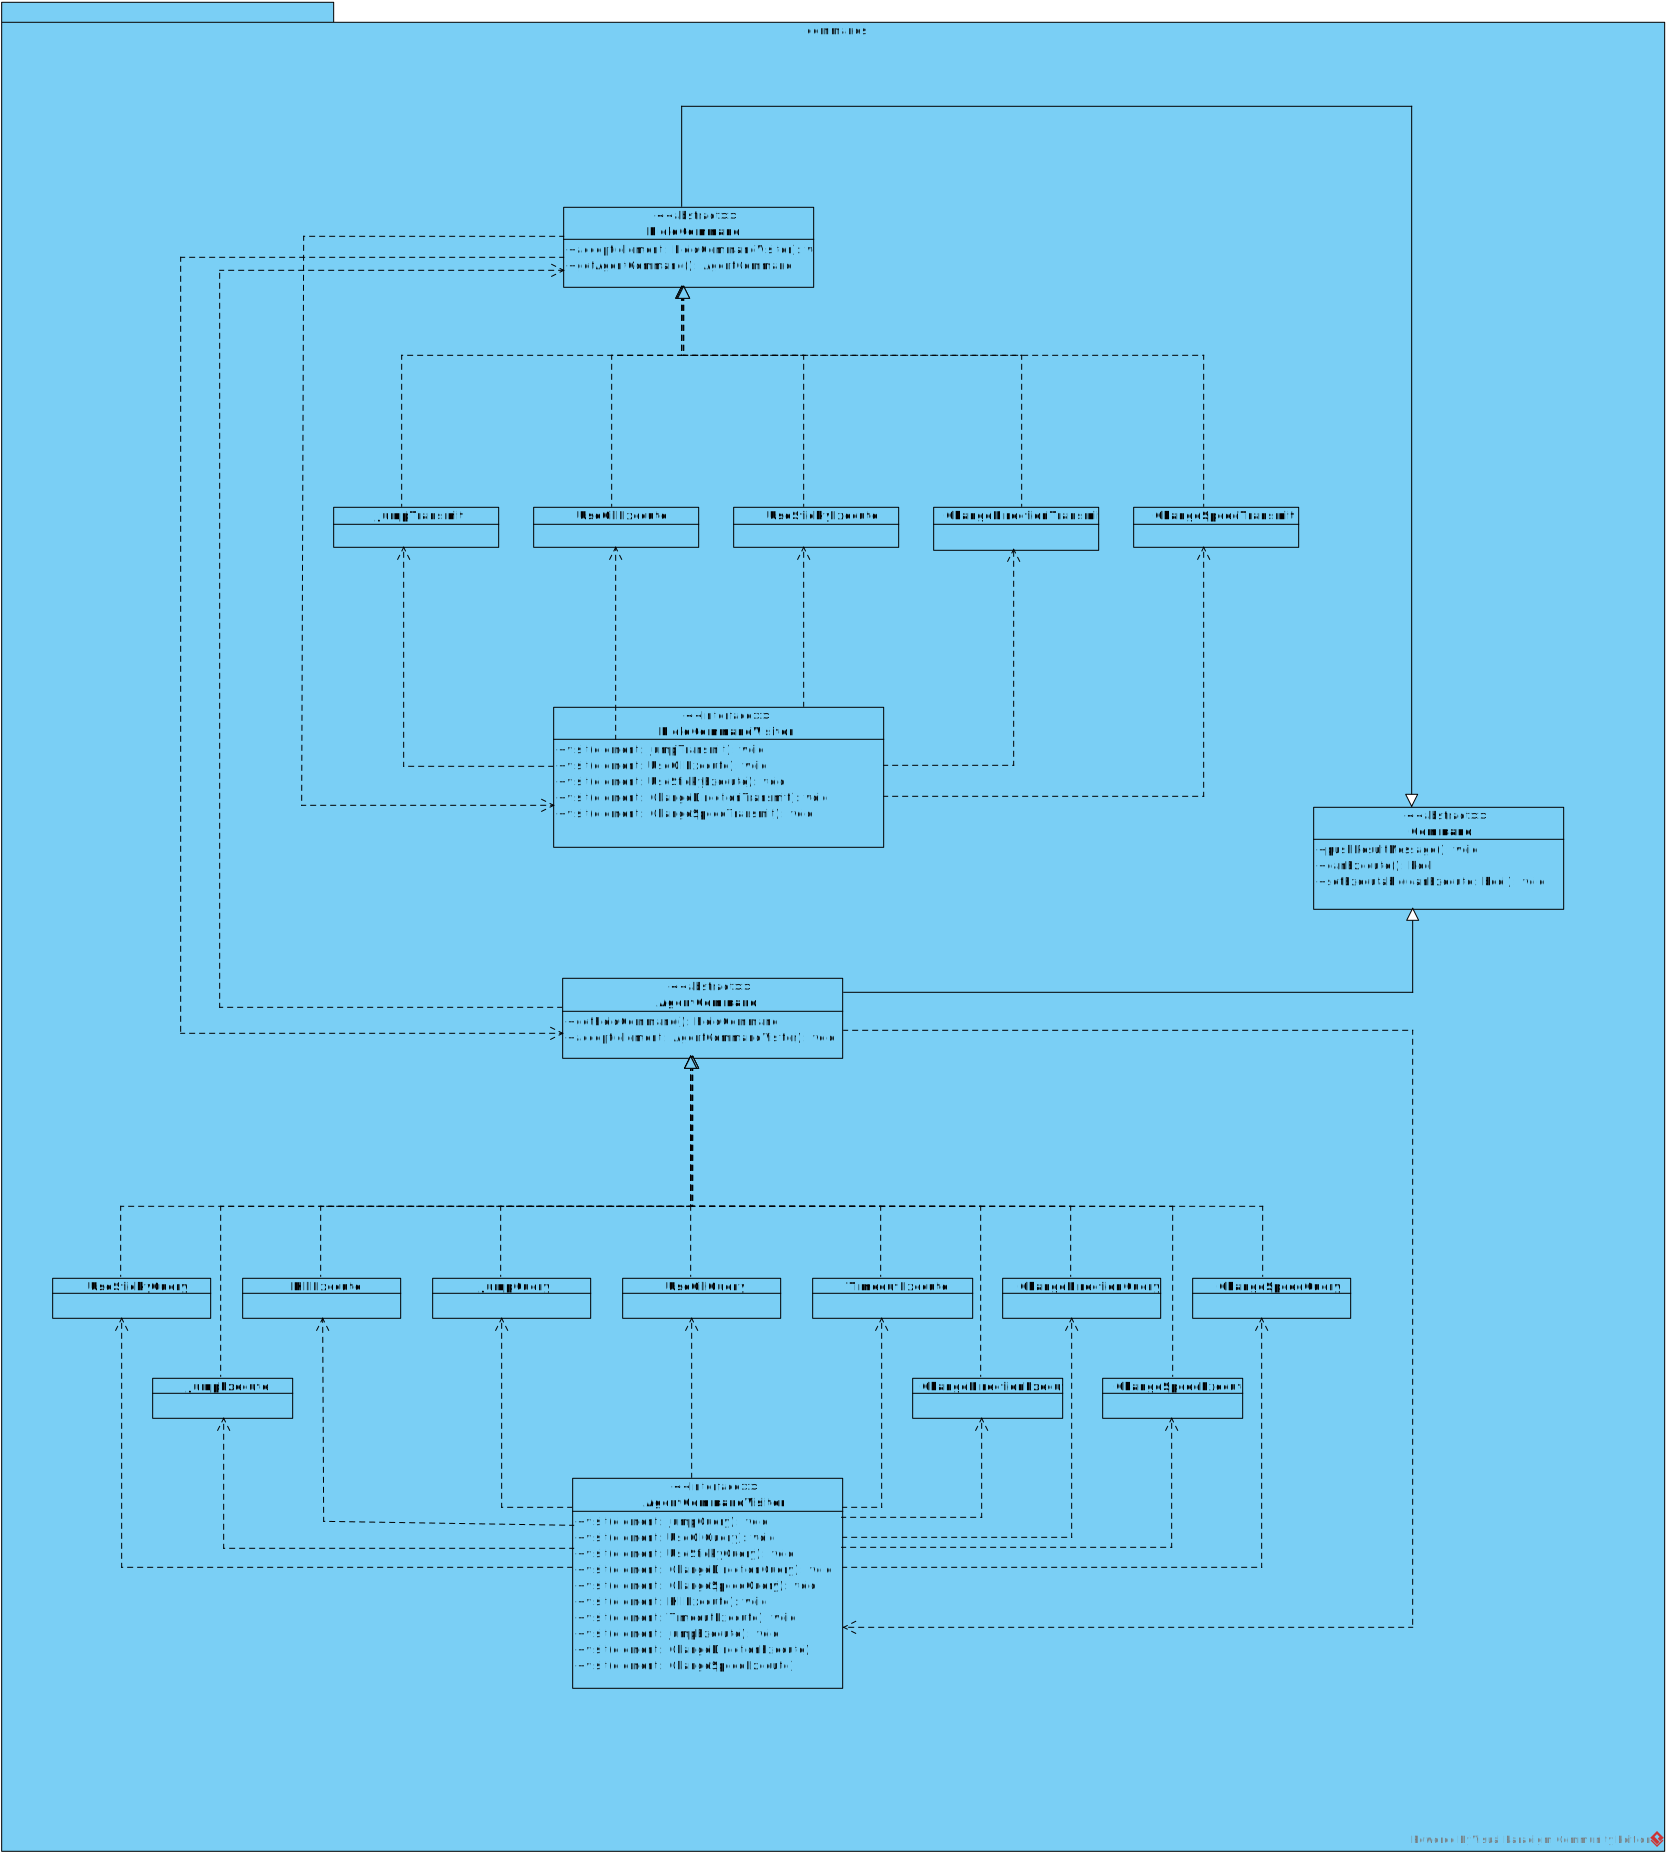
\includegraphics[width=\linewidth]{chapters/chapter04/ClassCommands.pdf}
		\caption{Commands package osztálydiagram}
		\label{Commands package osztálydiagram}
	\end{center}
\end{figure}


\begin{figure}[h]
	\begin{center}
		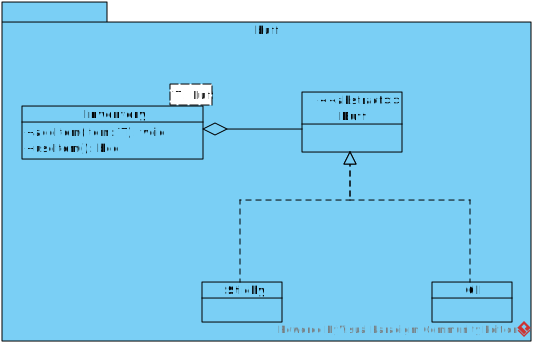
\includegraphics[width=\linewidth]{chapters/chapter04/ClassBuff.pdf}
		\caption{Buff package osztálydiagram}
		\label{Buff package osztálydiagram}
	\end{center}
\end{figure}


\begin{figure}[h]
	\begin{center}
		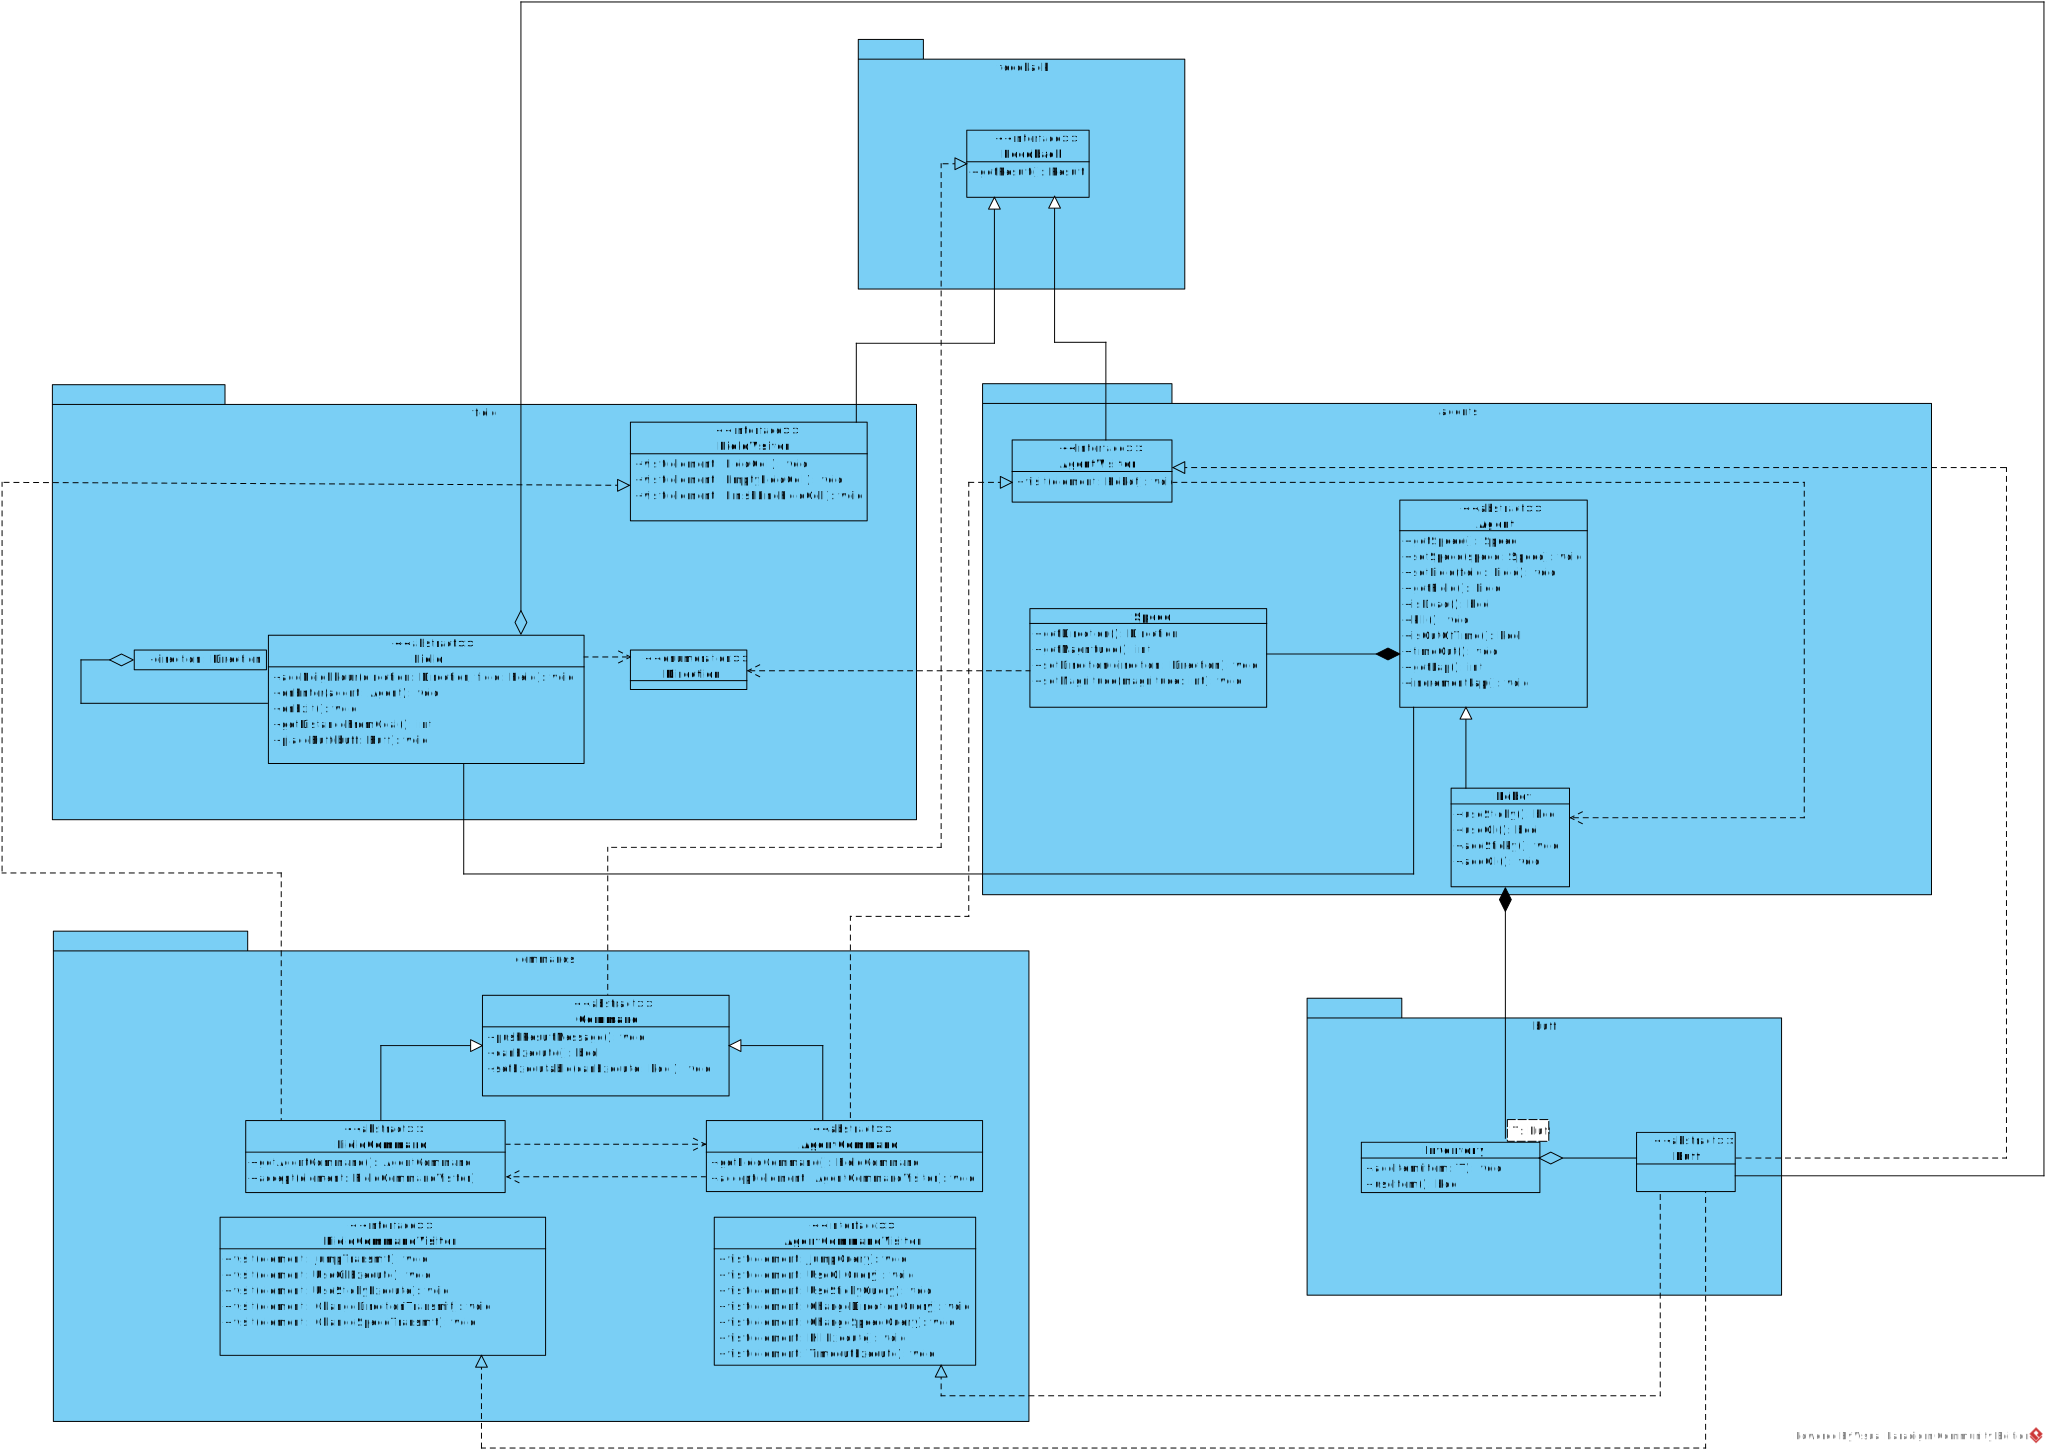
\includegraphics[width=\linewidth]{chapters/chapter04/ClassInterpackage.pdf}
		\caption{Packagek közti függőségek osztálydiagramja}
		\label{Packagek közti függőségek osztálydiagramja}
	\end{center}
\end{figure}

\clearpage

\section{Osztályok leírása}

\subsection{Agent (Abstract)}
\begin{itemize}

\item Felelősség\\
A pályán lévő összes ágens közös viselkedését valósítja meg: tárolja azoknak a sebességét, azt a \textbf{Fieldet}, amelyen éppen áll. Ezen felül számon tartja azt is, hogy az \textbf{Agent} élő vagy halott állapotban van-e, illetve hogy elfogyott-e már az adott \textbf{Agentre} osztott idő.

\item Ősosztályok\\
Nincs

\item Interfészek\\
AgentElement

\item Attribútumok\\
\begin{itemize}
    \item field: Field
    \item speed: Speed
    \item isDead: bool
    \item isOutOfTime: bool
    \item currentLeft: int
\end{itemize}

\item Metódusok\\

\begin{itemize}
    \item Speed getSpeed(): visszaadja az \textbf{Agent} sebességét
    \item void setSpeed(speed: Speed): beállítja az \textbf{Agent} sebességét
    \item Field getField(): visszaadja a mezőt, ahol az \textbf{Agent} áll
    \item void setField(field: Field): beállítja, hogy melyik mezőn áll az \textbf{Agent}
    \item bool isDead(): megmondja, hogy \textbf{Agent} halott-e
    \item void kill(): megöli az \textbf{Agentet}
    \item bool isOutOfTime(): megmondja, hogy az \textbf{Agentnek} van-e még ideje lépni
    \item void timeOut(): jelzi az \textbf{Agent} felé, hogy lejárt az ideje
    \item void getLap(): megmondja, hogy hányadik körben van az \textbf{Agent}
    \item void incrementLap(): növeli a kör számlálóját
\end{itemize}

\end{itemize}

\subsection{AgentCommand (Abstract)}
\begin{itemize}

\item Felelősség\\
Az Agentre vonatkozó parancsok közös ősosztálya, az azokra jellemző közös viselkedést valósítja meg.

\item Ősosztályok\\
Nincs

\item Interfészek\\
AgentVisitor

\item Attribútumok\\
Nincs

\item Metódusok\\

\begin{itemize}
    \item FieldCommand getFieldCommand(): amennyiben a parancsláncban szükeséges egy mezőnek átadni a parancsot, ezt állítja elő.
    \item void accept(element: AgentCommandVisitor): a \textbf{AgentCommandeket} módosítani képes objektumok ezen keresztül tudják ezt megtenni
\end{itemize}

\end{itemize}

\subsection{AgentCommandVisitor (Interface)}
\begin{itemize}

\item Felelősség\\
    Ezen interfészt implementáló osztályok képessé válnak az \textbf{AgentCommand} absztrakt osztály leszármazott osztályainak megváltoztatására képes azoknak publikus interfészén keresztül.

\item Ősosztályok\\
Nincs

\item Interfészek\\
Nincs

\item Attribútumok\\
Nincs

\item Metódusok\\

\begin{itemize}
    \item void visit(element: JumpQuery): egy \textbf{JumpQuery} objektum módosítására képes annak publikus interfészén keresztül
    \item void visit(element: UseOilQuery): egy \textbf{UseOilQuery} objektum módosítására képes annak publikus interfészén keresztül
    \item void visit(element: UseStickyQuery): egy \textbf{UseStickyQuery} objektum módosítására képes annak publikus interfészén keresztül
    \item void visit(element: ChangeDirectionQuery): egy \textbf{ChangeDirectionQuery} objektum módosítására képes annak publikus interfészén keresztül
    \item void visit(element: ChangeSpeedQuery): egy \textbf{ChangeSpeedQuery} objektum módosítására képes annak publikus interfészén keresztül
    \item void visit(element: KillExecute): egy \textbf{KillExecute} objektum módosítására képes annak publikus interfészén keresztül
    \item void visit(element: TimeoutExecute): egy \textbf{TimeoutExecute} objektum módosítására képes annak publikus interfészén keresztül
    \item void visit(element: JumpExecute): egy \textbf{JumpExecute} objektum módosítására képes annak publikus interfészén keresztül
    \item void visit(element: ChangeDirectionExecute): egy \textbf{ChangeDirectionExecute} objektum módosítására képes annak publikus interfészén keresztül
    \item void visit(element: ChangeSpeedExecute): egy \textbf{ChangeSpeedExecute} objektum módosítására képes annak publikus interfészén keresztül
\end{itemize}

\end{itemize}


\subsection{AgentElement (Interface)}
\begin{itemize}

\item Felelősség\\
Ez az interfész előírja, hogy az őt implementáló osztályoknak képesnek kell lennie \textbf{AgentVisitorok} és \textbf{AgentCommandek} fogadására. 

\item Ősosztályok\\
Nincs

\item Interfészek\\
Nincs

\item Attribútumok\\
Nincs

\item Metódusok\\

\begin{itemize}
    \item void accept(visitor: AgentVisitor): ez a metódus képes az \textbf{AgentVisitor} fogadására
    \item void accept(visitor: AgentCommand): ez a metódus képes az \textbf{AgentCommand} fogadására
\end{itemize}

\end{itemize}

\subsection{AgentVisitor (Interface)}
\begin{itemize}

\item Felelősség\\
Ezen interfészt implementáló osztályok képessé válnak az \textbf{Agent} absztrakt osztály leszármazott osztályainak megváltoztatására, azoknak publikus interfészén keresztül.

\item Ősosztályok\\
Nincs

\item Interfészek\\
Nincs

\item Attribútumok\\
Nincs

\item Metódusok\\

\begin{itemize}
    \item void visit(element: Robot): egy \textbf{Robot} módosítása annak publikus interfészén keresztül
\end{itemize}

\end{itemize}

\subsection{Buff (Abstract)}
\begin{itemize}

\item Felelősség\\
    Az összes releváns Visitornak biztosít egy üres implementációt, illetve közös ősosztály biztosít a játékban található \textbf{Buffoknak}. Ezek segítségével érhető el, hogy a játékos által kiadott parancsok és az \textbf{Agentek} tetszőlegesen módosíthatók legyenek. Interface collection.

\item Ősosztályok\\
Nincs

\item Interfészek\\
FieldCommandVisitor\\
AgentCommandVisitor\\
AgentVisitor\\

\item Attribútumok\\
Nincs

\item Metódusok\\
Nincs

\end{itemize}

\subsection{Command (Abstract)}
\begin{itemize}

\item Felelősség\\
    Az összes parancs közös ősosztály, tárolja azt az állapotot, hogy az adott parancs éppen futtatható-e. A parancsok általános feladata az \textbf{Agentek} és \textbf{Fieldek} közötti kommunikáció, illetva az azokkal való interakció megvalósítása. A parancsok részletes leírása a \textit{Command (Abstract)} pont alján található táblázatban látható.

\item Ősosztályok\\
Nincs

\item Interfészek\\
Nincs

\item Attribútumok\\
    \begin{itemize}
            \item canExecute: bool
    \end{itemize}

\item Metódusok\\

\begin{itemize}
    \item bool canExecute(): igazzal tér vissza, ha a parancs végrehajtható
    \item bool setExecutable(canExecute: bool): beállítja, hogy futtatható-e a parancs
\end{itemize}

\end{itemize}

\begin{tabularx}{\linewidth}{| p{4cm} | X | p{2.5cm} | l | p{1.2cm} | p{1.2cm} |}
\hline
\textbf{Név} & \textbf{Felelősség} & \textbf{Ősosztályok} & \textbf{Interfészek} &\parbox[t]{1.2cm}{\textbf{Attribú-tumok}} & \parbox[t]{1.2cm}{\textbf{Metó-dusok}} \tabularnewline
\hline\hline
\endhead
ChangeDirectionQuery & Egy robottól irányváltoztatást kérő parancs. Elő tudja állítani a megfelelő \textbf{ChangeDirectionTransmit} parancsot. & AgentCommand, Command & AgentVisitor & - & - \tabularnewline\hline

ChangeDirectionTransmit & Az az irányváltoztató parancs, amit egy cella módosítani tud a rajta található buffokkal. Elő tudja állítani a megfelelő \textbf{ChangeDirectionExecute} parancsot. &  FieldCommand, Command & FieldVisitor & - & -\tabularnewline\hline 

ChangeDirectionExecute & Az ugrást a \textbf{Roboton} ténylegesen végrehajtó parancs. & AgentCommand, Command & AgentVisitor & - & - \tabularnewline\hline

ChangeSpeedQuery & Egy robottól sebességváltoztatást kérő parancs. Elő tudja állítani a megfelelő \textbf{ChangeSpeedTransmit} parancsot. & AgentCommand, Command & AgentVisitor & - & - \tabularnewline\hline

ChangeSpeedTransmit & Az a sebességváltoztató parancs, amit egy cella módosítani tud a rajta található buffokkal. Elő tudja állítani a megfelelő \textbf{ChangeSpeedExecute} parancsot. &  FieldCommand, Command & FieldVisitor & - & -\tabularnewline\hline

ChangeSpeedExecute & A sebességváltoztatást a \textbf{Roboton} ténylegesen végrehajtó parancs. & AgentCommand, Command & AgentVisitor & - & - \tabularnewline\hline

JumpQuery & Egy robottól ugrás kezdeményezését kérő parancs. Lekérdezi és tárolja a robot aktuális sebességét. Elő tudja állítani a megfelelő \textbf{JumpTransmit} parancsot. & AgentCommand, Command & AgentVisitor & - & - \tabularnewline\hline

JumpTransmit & Az az ugróparancs, amit egy cella módosítani tud a rajta található buffokkal. Lekérdezi a cellától az ugrás kezdetét és célját, és tárolja ezeket. Elő tudja állítani a megfelelő \textbf{JumpExecute} parancsot. &  FieldCommand, Command & FieldVisitor & - & -\tabularnewline\hline 

JumpExecute & Az ugrást a \textbf{Roboton}, a kezdő és cél cellán ténylegesen végrehajtó parancs. & AgentCommand, Command & AgentVisitor & - & - \tabularnewline\hline

KillExecute & Egy \textbf{Robotot} a játékból kiiktatni képes parancs. & AgentCommand, Command & AgentVisitor & - & - \tabularnewline\hline

TimoutExecute & Egy \textbf{Robotnak} jelzi, hogy elfogyott a rá kijelölt teljes időtartam. & AgentCommand, Command & AgentVisitor & - & - \tabularnewline\hline

UseOilQuery & Egy \textbf{Robotot} arra utasít, hogy helyezzen egy \textbf{Oil} buffot arra a mezőre, amelyen áll. Lekérdezi, hogy a robotnak van-e elérhető \textbf{Oil} készlete, és ezt tárolja. Elő tudja állítani a megfelelő \textbf{UseOilExecute} parancsot. & AgentCommand, Command & AgentVisitor & - & - \tabularnewline\hline

UseOilExecute & Egy \textbf{Oil} buffot helyez el a cellán. &  FieldCommand, Command & FieldVisitor & - & -\tabularnewline\hline

UseStickyQuery & Egy \textbf{Robotot} arra utasít, hogy helyezzen egy \textbf{Sticky} buffot arra a mezőre, amelyen áll. Lekérdezi, hogy a robotnak van-e elérhető \textbf{Sticky} készlete, és ezt tárolja. Elő tudja állítani a megfelelő \textbf{UseStickyExecute} parancsot. & AgentCommand, Command & AgentVisitor & - & - \tabularnewline\hline

UseStickyExecute & Egy \textbf{Sticky} buffot helyez el a cellán. &  FieldCommand, Command & FieldVisitor & - & -\tabularnewline\hline
\end{tabularx}

\subsection{Direction}
\begin{itemize}

\item Felelősség\\
A pályán értelmezett lehetséges irányokat jelképező enumerált típus.

\item Ősosztályok\\
Nincs

\item Interfészek\\
Nincs

\item Attribútumok\\
Nincs

\item Metódusok\\
Nincs

\end{itemize}

\subsection{Displacement}
\begin{itemize}

\item Felelősség\\
Az elmozdulást kezelő osztály, mely a kezdeti és végpont mezőket tárolja.

\item Ősosztályok\\
Nincs

\item Interfészek\\
Nincs

\item Attribútumok\\
    \begin{itemize}
            \item start: Field
            \item goal: Field
    \end{itemize}

\item Metódusok\\

\begin{itemize}
    \item Field getStart(): visszaadja a kezdeti mezőt
    \item Field getGoal(): visszaadja az érkezési mezőt
\end{itemize}

\end{itemize}

\subsection{EmptyFieldCell}
\begin{itemize}

\item Felelősség\\
Az \textbf{EmptyFieldCell} osztály példányai a pálya azon részeit tárolja, amelyre lépve a \textbf{Robotok} kiesnek a játékból. Az ő felelőssége a robotnak elküldeni azt a parancsot, ami ezt a hatást előidézi (\textbf{KillExecute}).

\item Ősosztályok\\
Field

\item Interfészek\\
FieldElement

\item Attribútumok\\
Nincs

\item Metódusok\\
Nincs

\end{itemize}

\subsection{Field (Abstract)}
\begin{itemize}

\item Felelősség\\
    A pályát alkotó mezőtípusok közös ősosztálya, biztosítja a közös funkciók megvalósítását. Tárolja a rajta álló robotot, illetve referenciákat a szomszédos mezőkre, amiket a megfelelő \textbf{Direction} megadásával érhetünk el. Tartalmazza ezen felül a céltól való távolságot, amelyet a nyertes meghatározására használhatunk. Az ő felelőssége annak a cellának a megkeresése, amelyre egy \textbf{Robot} ugorhat. 

\item Ősosztályok\\
Nincs

\item Interfészek\\
Nincs

\item Attribútumok\\
    \begin{itemize}
            \item agent: Agent
            \item distanceFromGoal: int 
            \item buffs: Buff[]
            \item neighbours: Map<Direction, Field>
    \end{itemize}

\item Metódusok\\

\begin{itemize}
    \item void addNeighbour(direction: Direction, field: Field): hozzáadja a mezőhöz a megfelelő szomszédot a megfelelő irányban.
    \item void onEnter(agent: Agent): lekezeli azt az esetet, amikor egy \textbf{Agent} a cellára lép: beállítja a megfelelő referenciákat (mind az \textbf{Agentben}, mint önmagában). Ezen felül meghívja a rálépő \textbf{Agent} \textit{accept(AgentVisitor)} metódusát az összes, a mezőn található \textbf{Buffal}. 
    \item void onExit(): lekezeli azt az esetet, amikor egy \textbf{Agent} elhagyja a mezőt
    \item int getDistanceFromGoal(): megmondja, hogy a mező hány mezőre van a céltól.
    \item void placeBuff(buff: Buff): a paraméterben megadott buffot a mezőre teszi
    \item Displacement getDisplacement(speed: Speed): kiszámolja, hogy adott sebességgel melyik másik \textbf{Fieldre} lehet ugrani.
\end{itemize}

\end{itemize}

\subsection{FieldCell}
\begin{itemize}

\item Felelősség\\
    Ezen osztály példányai alkotják a pálya legnagyobb részét: minden olyan cella, amely nem a célvonal része, illetve nem a pálya szélét alkotja ilyen típusú. A \textbf{Field} osztály által implementált tulajdonságok mellett A cellán átmenő parancsokat módosíthatja a rajta található
    \textbf{Buffokal}, majd a módosított parancsokat továbbítja a rajta álló \textbf{Agent} felé.

\item Ősosztályok\\
Field

\item Interfészek\\
(Field) - FieldElement

\item Attribútumok\\
Nincs

\item Metódusok\\
Nincs

\end{itemize}

\subsection{FieldCommand (Abstract)}
\begin{itemize}

\item Felelősség\\
    A \textbf{Fieldre} vonatkozó parancsok közös ősosztálya, az azokra jellemző közös viselkedést valósítja meg.

\item Ősosztályok\\
Nincs

\item Interfészek\\
FieldVisitor

\item Attribútumok\\
Nincs

\item Metódusok\\

\begin{itemize}
    \item AgentCommand getAgentCommand(): amennyiben a parancsláncban szükeséges egy \textbf{Agentnek} átadni a parancsot, ezt állítja elő.
    \item void accept(element: FieldCommandVisitor): a \textbf{FieldCommandeket} módosítani képes objektumok ezen keresztül tudják ezt megtenni\end{itemize}

\end{itemize}

\subsection{FieldCommandVisitor (Interface)}
\begin{itemize}

\item Felelősség\\
    Ezen interfészt implementáló osztályok képessé válnak a \textbf{FieldCommand} absztrakt osztály leszármazott osztályainak megváltoztatására képes azoknak publikus interfészén keresztül.

\item Ősosztályok\\
Nincs

\item Interfészek\\
Nincs

\item Attribútumok\\
Nincs

\item Metódusok\\

\begin{itemize}
    \item void visit(element: JumpTransmit): egy JumpTransmit objektum módosítására képes annak publikus interfészén keresztül
    \item void visit(element: UseOilExecute): egy UseOilExecute objektum módosítására képes annak publikus interfészén keresztül
    \item void visit(element: UseStickyExecute): egy UseStickyExecute objektum módosítására képes annak publikus interfészén keresztül
    \item void visit(element: ChangeDirectionTransmit): egy ChangeDirectionTransmit objektum módosítására képes annak publikus interfészén keresztül
    \item void visit(element: ChangeSpeedTransmit): egy ChangeSpeedTransmit objektum módosítására képes annak publikus interfészén keresztül
\end{itemize}

\end{itemize}

\subsection{FieldElement (Interface)}
\begin{itemize}

\item Felelősség\\
    Ez az interfész előírja, hogy az őt implementáló osztályoknak képesnek kell lennie \textbf{FieldVisitorok} és \textbf{FieldCommandek} fogadására. 

\item Ősosztályok\\
Nincs

\item Interfészek\\
Nincs

\item Attribútumok\\
Nincs

\item Metódusok\\

\begin{itemize}
    \item void accept(visitor: FieldVisitor): ez a metódus képes a \textbf{FieldVisitor} fogadására
    \item void accept(visitor: FieldCommand): ez a metódus képes a \textbf{FieldCommand} fogadására
\end{itemize}

\end{itemize}

\subsection{FinishLineFieldCell}
\begin{itemize}

\item Felelősség\\
    A célt jelző mezőtípus, a körök nyomonkövetésekor használt mező. Viselkedése egyébként megegyezik a \textbf{FieldCellével}.

\item Ősosztályok\\
Field

\item Interfészek\\
(Field) - FieldElement

\item Attribútumok\\
Nincs

\item Metódusok\\
Nincs

\end{itemize}

\subsection{FieldVisitor (Interface)}
\begin{itemize}

\item Felelősség\\
Ezen interfészt implementáló osztályok képessé válnak a Field absztrakt osztály leszármazott osztályainak módosítására, megváltoztatására, azoknak publikus interfészén keresztül.

\item Ősosztályok\\
Nincs

\item Interfészek\\
Nincs

\item Attribútumok\\
Nincs

\item Metódusok\\

\begin{itemize}
    \item void visit(element: FieldCell): egy \textbf{FieldCell} objektum módosítására képes annak publikus interfészén keresztül
    \item void visit(element: EmptyFieldCell): meglátogat egy \textbf{EmptyFieldCell} objektumot
    \item void visit(element: FinishLineFieldCell): egy \textbf{FinishLineFieldCell} objektum módosítására képes annak publikus interfészén keresztül
\end{itemize}

\end{itemize}

\subsection{Inventory<T>}
\begin{itemize}

\item Felelősség\\
    \textbf{Buffok} tárolására alkalmas tároló: számon tartja az elérhető buffok számát, így csak akkor használható, amikor nem üres.

\item Ősosztályok\\
Nincs

\item Interfészek\\
Nincs

\item Attribútumok\\
\begin{itemize}
    \item buffs: T[]
\end{itemize}

\item Metódusok\\

\begin{itemize}
    \item void addItem(item: T): hozzáad egy T típusú itemet az Inventory<T>-hez.
    \item bool useItem(): használja az Inventory<T>-ben tárolt itemet, amennyiben nem üres igazzal tér vissza, különben hamis.
\end{itemize}

\end{itemize}

\subsection{Robot}
\begin{itemize}

\item Felelősség\\
    A pályán elhelyezkedő egyik \textbf{Agent} típus. Az ősosztályban megvalósított tulajdonságokon kívül rendelkezik \textbf{Sticky} és \textbf{Oil} \textbf{Inventorykkal}, amelyeket a \textbf{Robot} tetszőlegesen használhat, ha azok nem üresek.

\item Ősosztályok\\
Agent

\item Interfészek\\
(Agent) - AgentElement

\item Attribútumok\\
\begin{itemize}
    \item stickyInventory: Inventory<Sticky>
    \item oilInventory: Inventory<Oil>
    \item buffs: Buff[]
\end{itemize}
\end{itemize}

\subsection{Speed}
\begin{itemize}

\item Felelősség\\
    A sebesség tárolására alkalmas osztály, amely egy irányt (\textbf{Direction}) és egy nagyságot tárol.

\item Ősosztályok\\
Nincs

\item Interfészek\\
Nincs

\item Attribútumok\\
\begin{itemize}
    \item direction: Direction
    \item magnitude: int

\end{itemize}

\item Metódusok\\

\begin{itemize}
    \item Direction getDirection(): a sebesség irányát adja vissza
    \item int getMagnitude(): a sebesség nagyságát adja vissza
    \item void setDirection(dir: Direction): beállítja a sebesség irányát
    \item void setMagnitude(magnitude: int): beállítja a sebesség nagyságát
\end{itemize}

\end{itemize}

\clearpage



\section{Szekvencia diagramok}

\begin{figure}[h]
	\begin{center}
		\includegraphics[width=\textwidth]{chapters/chapter04/agentsRobotacceptAgentCommand.pdf}
		\caption{Robot utasítást fogad}
		\label{fig:agents.Robot.accept}
	\end{center}
\end{figure}

\begin{figure}[h]
	\begin{center}
		\includegraphics[width=\textwidth]{chapters/chapter04/agentsRobotaddOil.pdf}
		\caption{Robot felvesz a készletébe egy olajfoltot}
		\label{fig:agents.Robot.addOil}
	\end{center}
\end{figure}

\begin{figure}[h]
	\begin{center}
		\includegraphics[width=\textwidth]{chapters/chapter04/agentsRobotaddSticky.pdf}
		\caption{Robot felvesz a készletébe egy ragacsfoltot}
		\label{fig:agents.Robot.addSticky}
	\end{center}
\end{figure}

\begin{figure}[h]
	\begin{center}
		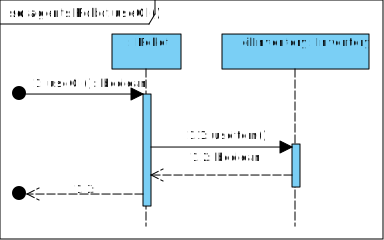
\includegraphics[width=\textwidth]{chapters/chapter04/agentsRobotuseOil.pdf}
		\caption{Robot felhasználja a készletében lévő olajfoltot ha van}
		\label{fig:agents.Robot.useOil}
	\end{center}
\end{figure}

\begin{figure}[h]
	\begin{center}
		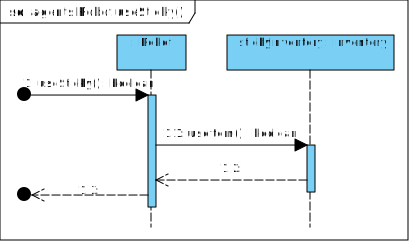
\includegraphics[width=\textwidth]{chapters/chapter04/agentsRobotuseSticky.pdf}
		\caption{Robot felhasználja a készletében lévő ragacsfoltot ha van}
		\label{fig:agents.Robot.useSticky}
	\end{center}
\end{figure}

\begin{figure}[h]
	\begin{center}
		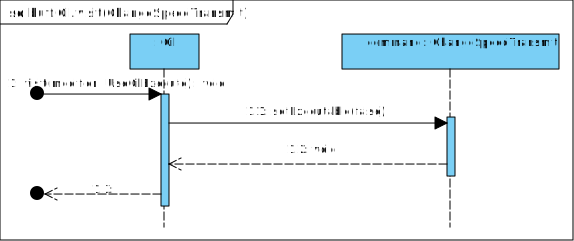
\includegraphics[width=\textwidth]{chapters/chapter04/buffOilvisitChangeSpeedTransmit.pdf}
		\caption{Olajfolt megakadályozza a sebesség nagyságának változtatását}
		\label{fig:buff.Oil.visit}
	\end{center}
\end{figure}

\begin{figure}[h]
	\begin{center}
		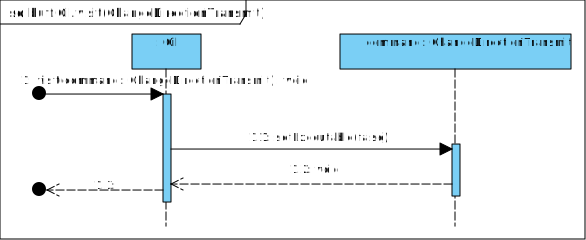
\includegraphics[width=\textwidth]{chapters/chapter04/buffOilvisitChangeDirectionTransmit.pdf}
		\caption{Olajfolt megakadályozza a sebesség irányának megváltoztatását}
		\label{fig:buff.Oil.visit2}
	\end{center}
\end{figure}

\begin{figure}[h]
	\begin{center}
		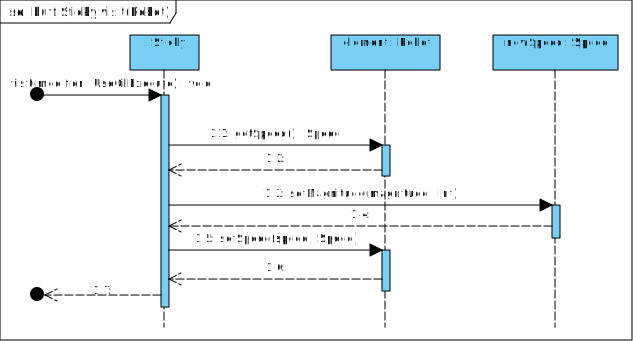
\includegraphics[width=\textwidth]{chapters/chapter04/buffStickyvisitRobot.pdf}
		\caption{Ragacs megfelezi a sebességet}
		\label{fig:buff.Sticky.visit}
	\end{center}
\end{figure}

\begin{figure}[h]
	\begin{center}
		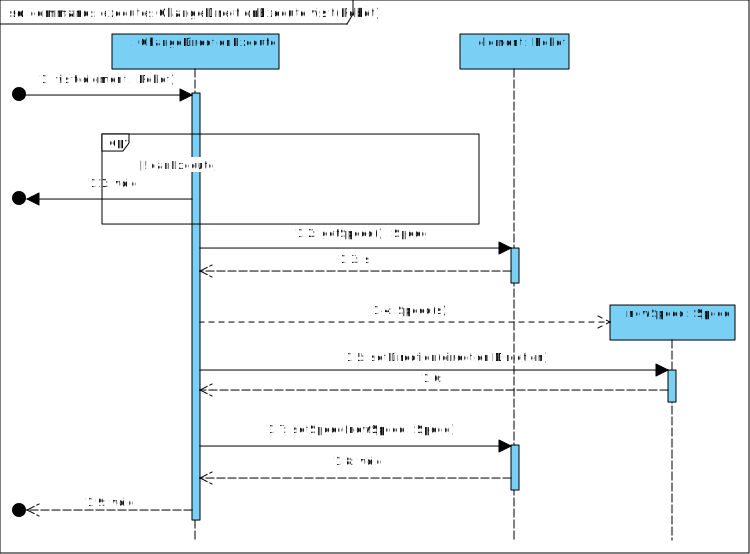
\includegraphics[width=\textwidth]{chapters/chapter04/commandsexecutesChangeDirectionExecutevisitRobot.pdf}
		\caption{Robot irányváltoztatásának végrehajtása}
		\label{fig:command.executes.ChangeDirectionExecute.visit}
	\end{center}
\end{figure}

\begin{figure}[h]
	\begin{center}
		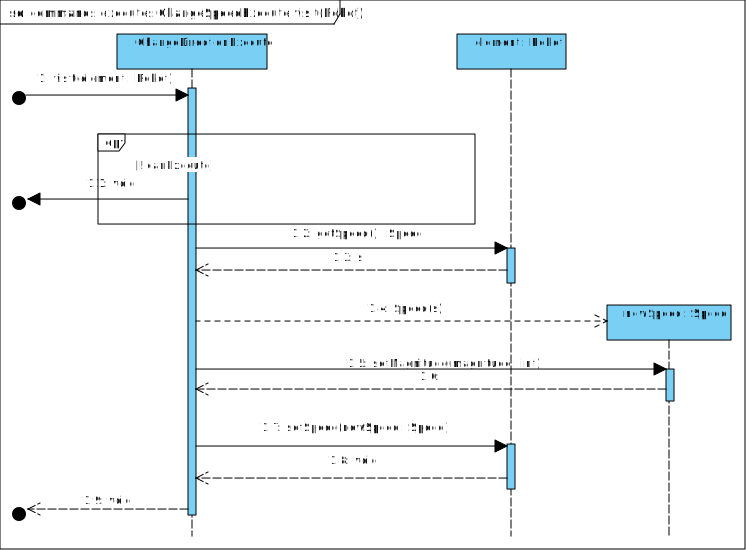
\includegraphics[width=\textwidth]{chapters/chapter04/commandsexecutesChangeSpeedExecutevisitRobot.pdf}
		\caption{Robot sebességnagyságának megváltoztatása}
		\label{fig:command.executes.ChangeSpeedExecute.visit}
	\end{center}
\end{figure}

\begin{figure}[h]
	\begin{center}
		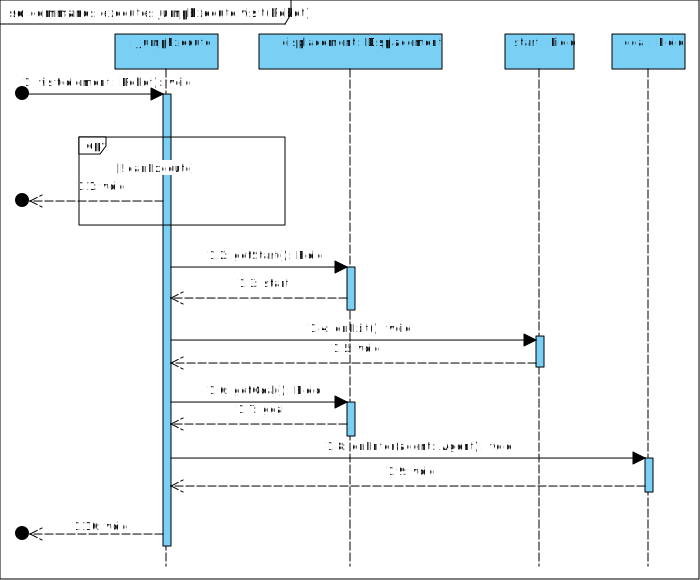
\includegraphics[width=\textwidth]{chapters/chapter04/commandsexecutesJumpExecutevisitRobot.pdf}
		\caption{Robot ugrásának végrehajtása}
		\label{fig:command.executes.JumpExecute.visit}
	\end{center}
\end{figure}

\begin{figure}[h]
	\begin{center}
		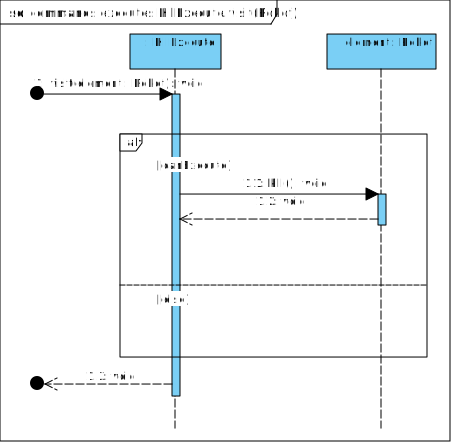
\includegraphics[width=\textwidth]{chapters/chapter04/commandsexecutesKillExecutevisitRobot.pdf}
		\caption{Robot megölésének végrehajtása}
		\label{fig:command.executes.KillExecute.visit}
	\end{center}
\end{figure}

\begin{figure}[h]
	\begin{center}
		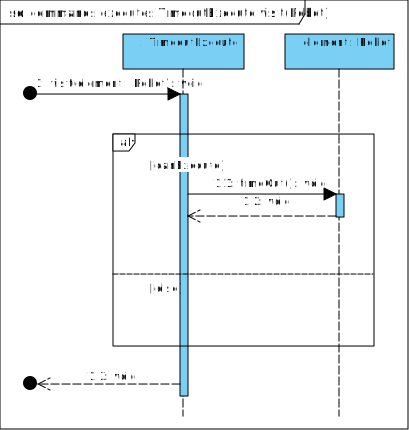
\includegraphics[width=\textwidth]{chapters/chapter04/commandsexecutesTimeoutExecutevisitRobot.pdf}
		\caption{Robot idő lejártának végrehajtása}
		\label{fig:command.executes.TimeoutExecute.visit}
	\end{center}
\end{figure}

\begin{figure}[h]
	\begin{center}
		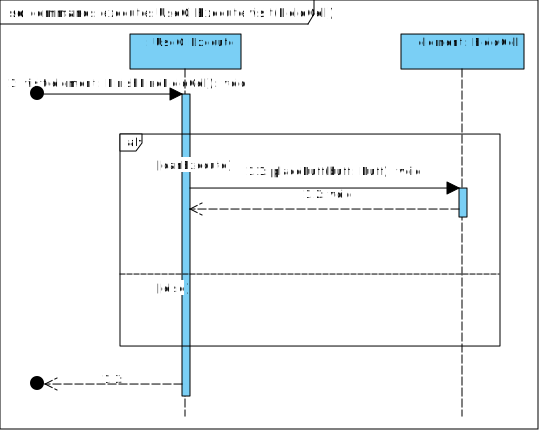
\includegraphics[width=\textwidth]{chapters/chapter04/commandsexecutesUseOilExecutevisitFieldCell.pdf}
		\caption{Robot lehelyezi az Olaj foltot a mezőre}
		\label{fig:command.executes.UseOilExecute.visit}
	\end{center}
\end{figure}

\begin{figure}[h]
	\begin{center}
		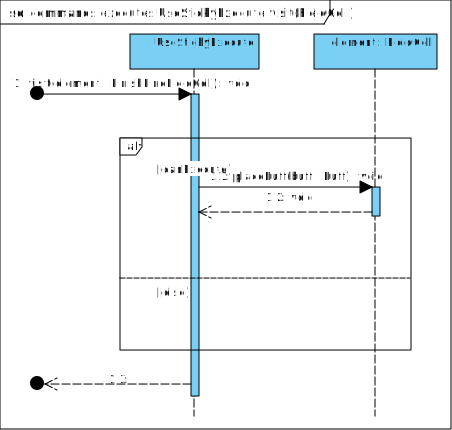
\includegraphics[width=\textwidth]{chapters/chapter04/commandsexecutesUseStickyExecutevisitFieldCell.pdf}
		\caption{Robot lehelyezi a Ragacs foltot a mezőre}
		\label{fig:command.executes.UseStickyExecute.visit}
	\end{center}
\end{figure}

\clearpage

\begin{figure}[h]
	\begin{center}
		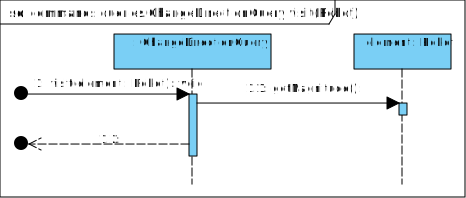
\includegraphics[width=\textwidth]{chapters/chapter04/commandsqueriesChangeDirectionQueryvisitRobot.pdf}
		\caption{Robot irányváltásra való felkérése}
		\label{fig:command.executes.ChangeDirectionQuery.visit}
	\end{center}
\end{figure}


\begin{figure}[h]
	\begin{center}
		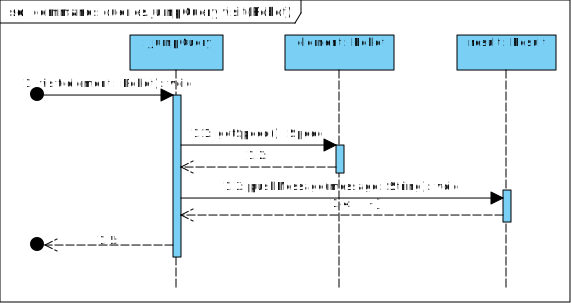
\includegraphics[width=\textwidth]{chapters/chapter04/commandsqueriesJumpQueryvisitRobot.pdf}
		\caption{Robot ugrásra azaz helyzetmódosításra való felkérése}
		\label{fig:command.executes.JumpQuery.visit}
	\end{center}
\end{figure}

\begin{figure}[h]
	\begin{center}
		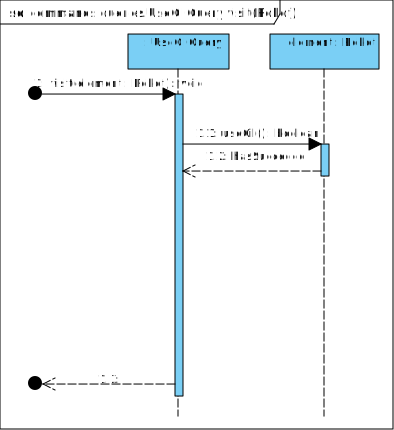
\includegraphics[width=\textwidth]{chapters/chapter04/commandsqueriesUseOilQueryvisitRobot.pdf}
		\caption{Robotot Olaj lehelyezésére való felkérése}
		\label{fig:command.executes.UseOilQuery.visit}
	\end{center}
\end{figure}

\begin{figure}[h]
	\begin{center}
		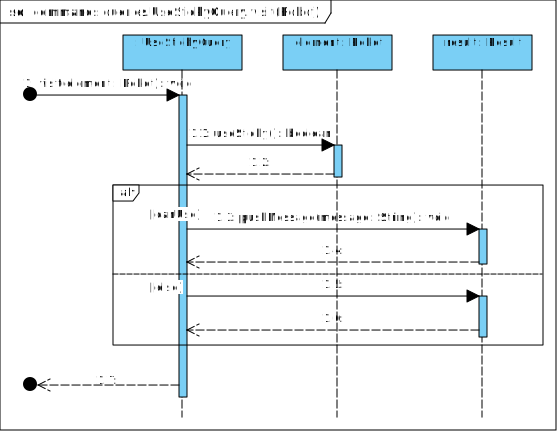
\includegraphics[width=\textwidth]{chapters/chapter04/commandsqueriesUseStickyQueryvisitRobot.pdf}
		\caption{Robotot Ragacs lehelyezésére való felkérése}
		\label{fig:command.executes.UseStickyQuery.visit}
	\end{center}
\end{figure}

\begin{figure}[h]
	\begin{center}
		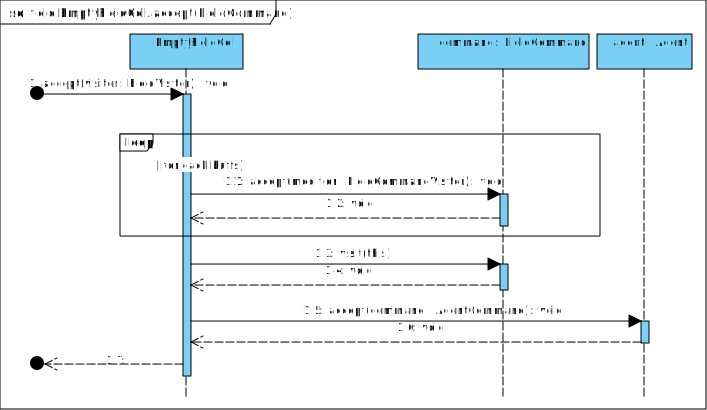
\includegraphics[width=\textwidth]{chapters/chapter04/fieldEmptyFieldCellacceptFieldCommand.pdf}
		\caption{Üres pályamező utasításfeldolgozása}
		\label{fig:field.EmptyFieldCell.accept}
	\end{center}
\end{figure}

\begin{figure}[h]
	\begin{center}
		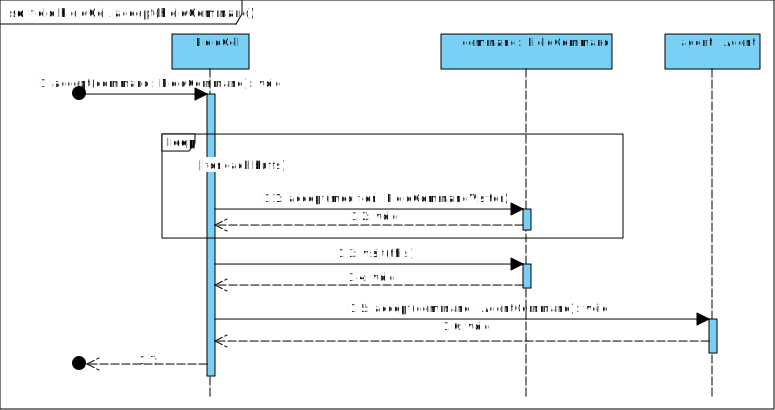
\includegraphics[width=\textwidth]{chapters/chapter04/fieldFieldCellacceptFieldCommand.pdf}
		\caption{Pályamező utasításfeldolgozása}
		\label{fig:field.FieldCell.accept}
	\end{center}
\end{figure}

\begin{figure}[h]
	\begin{center}
		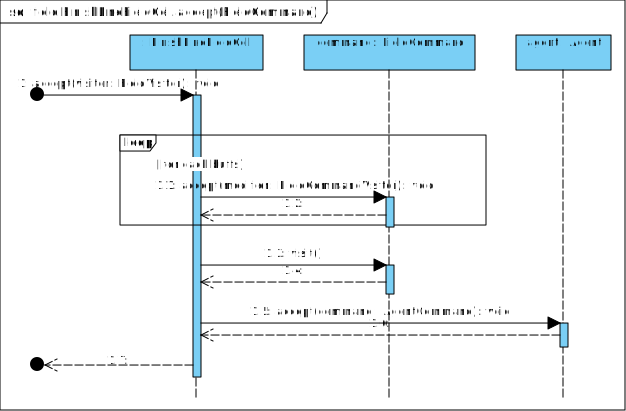
\includegraphics[width=\textwidth]{chapters/chapter04/fieldFinishLineFieldCellacceptFieldCommand.pdf}
		\caption{Start/célvonal pályamező utasításfeldolgozása}
		\label{fig:field.FinishLineFieldCell.accept}
	\end{center}
\end{figure}

\clearpage

\section{State-chartok}
\begin{figure}[h]
	\begin{center}
		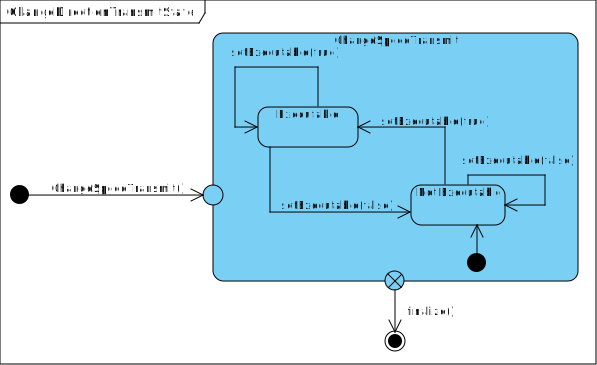
\includegraphics[width=\textwidth]{chapters/chapter04/ChangeDirectionTransmitState.pdf}
		\caption{ChangeDirectionTransmit osztály állapotdiagramja}
		\label{fig:state.ChangeDirectionTransmit}
	\end{center}
\end{figure}

\begin{figure}[h]
	\begin{center}
		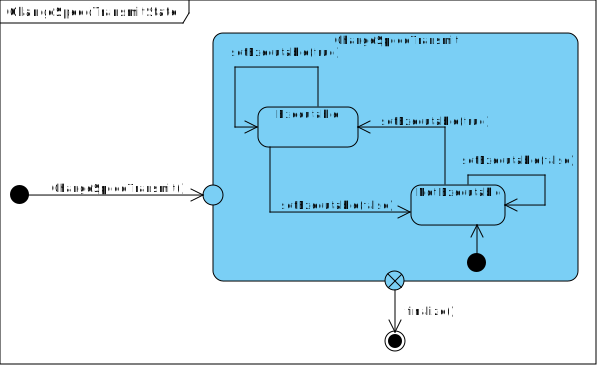
\includegraphics[width=\textwidth]{chapters/chapter04/ChangeSpeedTransmitState.pdf}
		\caption{ChangeSpeedTransmit osztály állapotdiagramja}
		\label{fig:state.ChangeSpeedTransmit}
	\end{center}
\end{figure}

\clearpage
%% Szglab4
% ===========================================================================
%
\section{Napló}

\begin{naplo}
	
	\bejegyzes
	{2015.03.04. ~8.00}
	{2 óra}
	{Nyári} 
	{Tevékenység: Elkészíti a Konzultációs jegyzőkönyvet.\newline } 
	
	
	\bejegyzes
	{2015.03.04 ~20.00}
	{2 óra}
	{Paral \newline Nyári \newline Szőke \newline Nagy} 
	{Értekezlet.
		Döntés: Feladatok felosztása az feladatok hozzárendelése a megfelelő emberekhez. A részletek megbeszélése, tervezés, koncepciók átgondolása.\newline } 
			
	
	\bejegyzes
	{2015.03.07. ~08.00}
	{4 óra}
	{Szőke} 
	{Tevékenység: Szekvenciadiagrammok szekció javítása.\newline } 
		
	\bejegyzes
	{2015.03.08 ~17.00}
	{1 óra}
	{Nagy} 
	{Tevékenység: Reviewra szánt idő a pull-requestekre.\newline } 
	
	\bejegyzes
	{2015.03.08. ~17.00}
	{1 óra}
	{Nyári} 
	{Tevékenység: Reviewra szánt idő a pull-requestekre.\newline } 
			
	\bejegyzes
	{2015.03.08. ~10.00}
	{1 óra}
	{Szőke} 
	{Tevékenység: Napló elkészítése.\newline } 
	
\end{naplo}





%\setcounter{chapter}{4}
%% Szglab4
% ===========================================================================
%
\chapter{Szkeleton tervezése}

\thispagestyle{fancy}

\section{A szkeleton modell valóságos use-case-ei}
\comment{A szkeletonnak, mint önálló programnak a működésével kapcsolatos use-case-ek.}

\subsection{Use-case diagram}

\begin{figure}[h]
\begin{center}
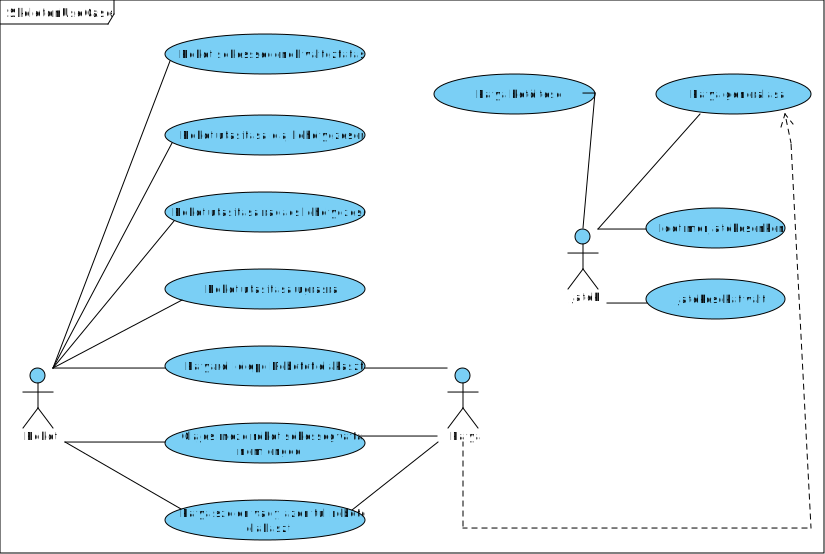
\includegraphics[width=\textwidth]{chapters/chapter05/SkeletonUseCase.pdf}
\caption{Szkeleton Use Case Diagram}
\label{fig:SzkeletonUseCase}
\end{center}
\end{figure}

\subsection{Use-case leírások}
%\comment{Minden use-case-hez külön}

\usecase%
{Új játék indítása}%
{Elindíthatunk egy új játékot}%
{Játékos, Játék}%
{A játékosok számának megadása után a Játékos kezdeményezheti a játéknak az elindítását}

\usecase%
{Játék megnyerése}%
{Játék végső helyzete alapján győztes eldöntése}%
{Játékos, Játék}%
{Ha minden Játékosnak lejár akkor a megtett út alapján eldől, hogy ki a győztes}

\usecase%
{Játék elvesztése}%
{Játék végső helyzete alapján vesztesek eldöntése}%
{Játékos, Játék}%
{Ha minden Játékosnak lejár akkor a megtett út alapján eldől, hogy kik a vesztesek}

\usecase%
{Játékparaméterek megadása}%
{Új játék paramétereinek megadása}%
{Játék}%
{Játékosok megadhatják, hogy hányan vannak, milyen időkorláttal kívánnak játszani}

\usecase%
{Pálya generálása}%
{Új játékpályát generálunk}%
{Játék, Játékos}%
{A Játékosok egy új pályát kívánnak generálni}

\usecase%
{Jelenlegi játék mentése}%
{Játék aktuállis állásának mentése}%
{Játék, Játékos}%
{A Játékosok valamilyen oknál kifolyólag később akarják folytatni a játékot}

\usecase%
{Mentett játék betöltáse}%
{Már elmentett jűték betöltése}%
{Játék, Játékos}%
{A Játékosok a régebben félbehagyott játékot folytathatják ahol abbahagyták}

\usecase%
{Időt mér játékosonkét}%
{Játékmenet és Játékosonkénti időnyilvántartás}%
{Játék}%
{Nyilvántartja a Játékosok még hátralévő idejét, és megállítja azokat akik már nem képhetnek}

\usecase%
{Játékosokat vált}%
{Játékosokat vált körönként}%
{Játék}%
{Játékost cserél körönként ha a játékos ugrott vagy lejárt az ideje}

\usecase%
{Robot sebességének változtatása}%
{A Játékos megváltoztathatja a Robotnak a sebességét}%
{Játékos, Robot}%
{A játékos körönként megváltoztathatja a Robotnak a sebességét}

\usecase%
{Robot utasítása olajnak a lehelyezése}%
{Játékos utasíthatja a Robotot, hogy helyezze le az olajfoltot}%
{Játékos, Robot}%
{A Játékos más játékosok hátráltatásának okán lehelyezhet a készletáéből egy olajfoltot}

\usecase%
{Robot utasítása ragacsnak a lehelyezése}%
{Játékos utasíthatja a Robotot, hogy helyezze le az ragacsfoltot}%
{Játékos, Robot}%
{A Játékos más játékosok hátráltatásának okán lehelyezhet a készletáéből egy ragacsfoltot}

\usecase%
{Robot utasítása ugrásra}%
{Játékos utasíthatja a Robotot, hogy végezze el az ugrást}%
{Játékos, Robot, Játék}%
{Játékos utasíthatja a Robotot, hogy végezze el az ugrást, amennyiben ezt nem teszi meg a Játék kikényszerítheti ezt a lépést}

\usecase%
{Olajos mező Robot sebességváltoztatást nem enged}%
{Ha olajos mezőn vagyunk akkor a mező nem engedi a lépést a robotnak}%
{Robot, Pálya}%
{Ha egy Robot rálép az olajra akkor a mező nem engedi neki a sebességváltoztatást}

\usecase%
{Ragacs mező Robot sebességet megfelez}%
{Ha ragacsos mezőn vagyunk akkor a mező megfelezi a Robot sebességét}%
{Robot, Pálya}%
{Ha egy Robot rálép a ragacsra akkor a mező megfelezi aa Robotnak a sebességét}

\usecase%
{Pályáról lelépő Robotot elakaszt}%
{Pályáról lelépő robotot elakasztjuk, nem léphet tovább}%
{Robot, Pálya}%
{Ha egy Robot kilép a pálya határain kívülre akkor elakasztja őt}

\section{A szkeleton kezelői felületének terve, dialógusok}
\comment{A szkeleton által elfogadott bemenetek , valamint a szöveges konzolon megjelenő kimenetek. A kiemenet formátuma olyan kell legyen, ami alapján a működés összevethető a korábbi szekvencia-diagramokkal.}

\section{Szekvencia diagramok a belső működésre}
\comment{A szkeletonban implementált szekvenciadiagramok. Tipikusan egy use-case egy diagram. Ezek megegyezhetnek a korábban specifikált diagramokkal, de az egyes életvonalakat (lifeline) egyértelműen a szkeletonban példányosított objektumokhoz kell tudni kötni. Azt kell megjeleníteni, hogy a szkeletonban létrehozott objektumok egymással hogyan fognak kommunikálni.}

\section{Kommunikációs diagramok}
\comment{A szkeletonban, az egyes szkeleton-use-case-ek futása során létrehozott objektumok és kapcsolataik bemutatására szolgáló diagramok. Ezek alapján valósítják meg a szkeleton fejlesztői az inicializáló kódrészleteket.}

%% Szglab4
% ===========================================================================
%
\section{Napló}

\begin{naplo}

\bejegyzes
{2010.03.21.~18:00~} % Kezdet
{2,5 óra} % Időtartam
{Horváth\newline
Németh\newline
Tóth\newline
Oláh} % Résztvevők
{Értekezlet. Döntés: Horváth elkészíti az osztálydiagramot, Oláh a use-case leírásokat.} % Leírás

\bejegyzes
{2010.03.23.~23:00~}
{5 óra}
{Németh}
{Tevékenység: Németh implementálja a tesztelő programokat.}

\bejegyzes
{...}
{...}
{...}
{...}


\end{naplo}



%\setcounter{chapter}{5}
%% Szglab4
% ===========================================================================
%
\chapter{Szkeleton beadás}

\thispagestyle{fancy}

\section{Fordítási és futtatási útmutató}

\subsection{Fájllista}
\begin{tabularx}{\linewidth}{| l | l | l | X |}
\hline
\textbf{Fájl neve} & \textbf{Méret} & \textbf{Keletkezés ideje} & \textbf{Tartalom} \tabularnewline
\hline \hline
\endhead
\fajl
{src/main/agents/AgentElement.java}
{161 byte}
{2015.02.27~06:09~}
{Az AgentElement interfész deklarációját tartalmazza.}

\fajl
{src/main/agents/Agent.java}
{875 byte}
{2015.02.27~06:09~}
{Az Agent osztály implementációját tartalmazza.}

\fajl
{src/main/agents/AgentVisitor.java}
{126 byte}
{2015.02.27~06:09~}
{Az AgentVisitor interfész deklarációját tartalmazza.}

\fajl
{src/main/agents/Robot.java}
{1171 byte}
{2015.02.27~06:09~}
{A Robot osztály implementációját tartalmazza.}

\fajl
{src/main/agents/Speed.java}
{1087 byte}
{2015.02.27~06:09~}
{A Speed osztály implementációját tartalmazza.}

\fajl
{src/main/buff/Buff.java}
{1404 byte}
{2015.02.27~06:09~}
{A Buff osztály implementációját tartalmazza.}

\fajl
{src/main/buff/Inventory.java}
{450 byte}
{2015.02.27~06:09~}
{Az Inventory osztály implementációját tartalmazza.}

\fajl
{src/main/buff/Oil.java}
{375 byte}
{2015.02.27~06:09~}
{Az Oil osztály implementációját tartalmazza.}

\fajl
{src/main/buff/Sticky.java}
{374 byte}
{2015.02.27~06:09~}
{A Sticky osztály implementációját tartalmazza.}

\fajl
{src/main/commands/AgentCommand.java}
{383 byte}
{2015.02.27~06:09~}
{Az AgentCommand osztály implementációját tartalmazza.}

\fajl
{src/main/commands/AgentCommandVisitor.java}
{490 byte}
{2015.02.27~06:09~}
{Az AgentCommandVisitor interfész deklarációját tartalmazza.}

\fajl
{src/main/commands/Command.java}
{654 byte}
{2015.02.27~06:09~}
{A Command osztály implementációját tartalmazza.}

\fajl
{src/main/commands/executes/ChangeDirectionExecute.java}
{1206 byte}
{2015.02.27~06:09~}
{A ChangeDirectionExecute osztály implementációját tartalmazza.}

\fajl
{src/main/commands/executes/ChangeSpeedExecute.java}
{1243 byte}
{2015.02.27~06:09~}
{A ChangeSpeedExecute osztály implementációját tartalmazza.}

\fajl
{src/main/commands/executes/JumpExecute.java}
{1262 byte}
{2015.02.27~06:09~}
{A JumpExecute osztály implementációját tartalmazza.}

\fajl
{src/main/commands/executes/KillExecute.java}
{616 byte}
{2015.02.27~06:09~}
{A KillExecute osztály implementációját tartalmazza.}

\fajl
{src/main/commands/executes/UseOilExecute.java}
{1143 byte}
{2015.02.27~06:09~}
{Az UseOilExecute osztály implementációját tartalmazza.}

\fajl
{src/main/commands/executes/UseStickyExecute.java}
{1176 byte}
{2015.02.27~06:09~}
{Az UseStickyExecute osztály implementációját tartalmazza.}

\fajl
{src/main/commands/FieldCommand.java}
{382 byte}
{2015.02.27~06:09~}
{A FieldCommand osztály implementációját tartalmazza.}

\fajl
{src/main/commands/FieldCommandVisitor.java}
{340 byte}
{2015.02.27~06:09~}
{A FieldCommandVisitor interfész deklarációját tartalmazza.}

\fajl
{src/main/commands/NoAgentCommandException.java}
{77 byte}
{2015.02.27~06:09~}
{A NoAgentCommandException osztály implementációját tartalmazza.}

\fajl
{src/main/commands/NoFieldCommandException.java}
{78 byte}
{2015.02.27~06:09~}
{A NoFieldCommandException osztály implementációját tartalmazza.}

\fajl
{src/main/commands/queries/ChangeDirectionQuery.java}
{803 byte}
{2015.02.27~06:09~}
{A ChangeDirectionQuery osztály implementációját tartalmazza.}

\fajl
{src/main/commands/queries/ChangeSpeedQuery.java}
{789 byte}
{2015.02.27~06:09~}
{A ChangeSpeedQuery osztály implementációját tartalmazza.}

\fajl
{src/main/commands/queries/JumpQuery.java}
{727 byte}
{2015.02.27~06:09~}
{A JumpQuery osztály implementációját tartalmazza.}

\fajl
{src/main/commands/queries/UseOilQuery.java}
{686 byte}
{2015.02.27~06:09~}
{Az UseOilQuery osztály implementációját tartalmazza.}

\fajl
{src/main/commands/queries/UseStickyQuery.java}
{704 byte}
{2015.02.27~06:09~}
{Az UseStickyQuery osztály implementációját tartalmazza.}

\fajl
{src/main/commands/transmits/ChangeDirectionTransmit.java}
{1008 byte}
{2015.02.27~06:09~}
{A ChangeDirectionTransmit osztály implementációját tartalmazza.}

\fajl
{src/main/commands/transmits/ChangeSpeedTransmit.java}
{1011 byte}
{2015.02.27~06:09~}
{A ChangeSpeedTransmit osztály implementációját tartalmazza.}

\fajl
{src/main/commands/transmits/JumpTransmit.java}
{1324 byte}
{2015.02.27~06:09~}
{A JumpTransmit osztály implementációját tartalmazza.}

\fajl
{src/main/feedback/Feedback.java}
{100 byte}
{2015.02.27~06:09~}
{A Feedback interfész deklarációját tartalmazza.}

\fajl
{src/main/feedback/NoFeedbackException.java}
{74 byte}
{2015.02.27~06:09~}
{A NoFeedbackException osztály implementációját tartalmazza.}

\fajl
{src/main/feedback/Result.java}
{554 byte}
{2015.02.27~06:09~}
{A Result osztály implementációját tartalmazza.}

\fajl
{src/main/field/Direction.java}
{80 byte}
{2015.02.27~06:09~}
{A Direction osztály implementációját tartalmazza.}

\fajl
{src/main/field/Displacement.java}
{335 byte}
{2015.02.27~06:09~}
{A Displacement osztály implementációját tartalmazza.}

\fajl
{src/main/field/EmptyFieldCell.java}
{952 byte}
{2015.02.27~06:09~}
{Az EmptyFieldCell osztály implementációját tartalmazza.}

\fajl
{src/main/field/FieldCell.java}
{630 byte}
{2015.02.27~06:09~}
{A FieldCell osztály implementációját tartalmazza.}

\fajl
{src/main/field/FieldElement.java}
{160 byte}
{2015.02.27~06:09~}
{A FieldElement interfész deklarációját tartalmazza.}

\fajl
{src/main/field/Field.java}
{1655 byte}
{2015.02.27~06:09~}
{A Field osztály implementációját tartalmazza.}

\fajl
{src/main/field/FieldVisitor.java}
{216 byte}
{2015.02.27~06:09~}
{A FieldVisitor interfész deklarációját tartalmazza.}

\fajl
{src/main/field/FinishLineFieldCell.java}
{614 byte}
{2015.02.27~06:09~}
{A FinishLineFieldCell osztály implementációját tartalmazza.}

\fajl
{src/main/game/AgentController.java}
{214 byte}
{2015.03.14~10:10~}
{Az AgentController osztály implementációját tartalmazza.}

\fajl
{src/main/game/ControllerListener.java}
{88 byte}
{2015.03.14~12:28~}
{A ControllerListener interfész deklarációját tartalmazza.}

\fajl
{src/main/game/GameCreator.java}
{2732 byte}
{2015.03.14~10:10~}
{A GameCreator osztály implementációját tartalmazza.}

\fajl
{src/main/game/Game.java}
{3291 byte}
{2015.03.14~10:10~}
{A Game osztály implementációját tartalmazza.}

\fajl
{src/main/game/HumanController.java}
{1887 byte}
{2015.03.14~10:10~}
{A HumanController osztály implementációját tartalmazza.}

\fajl
{src/main/game/KeyDispatcher.java}
{220 byte}
{2015.03.14~10:10~}
{A KeyDispatcher osztály implementációját tartalmazza.}

\fajl
{src/main/game/Map.java}
{1778 byte}
{2015.03.14~10:10~}
{A Map osztály implementációját tartalmazza.}

\fajl
{src/main/game/Player.java}
{660 byte}
{2015.03.14~10:10~}
{A Player osztály implementációját tartalmazza.}

\fajl
{src/main/Main.java}
{1367 byte}
{2015.02.12~23:16~}
{A Main osztály implementációját tartalmazza.}

\fajl
{src/test/TravisTester.java}
{162 byte}
{2015.02.13~00:27~}
{A TravisTester osztály implementációját tartalmazza.}

\end{tabularx}


\subsection{Fordítás}
\comment{A fenti listában szereplő forrásfájlokból milyen műveletekkel lehet a bináris, futtatható kódot előállítani. Az előállításhoz csak a 2. Követelmények c. dokumentumban leírt környezetet szabad előírni.}

\lstset{escapeinside=`', xleftmargin=10pt, frame=single, basicstyle=\ttfamily\footnotesize, language=sh}
\begin{lstlisting}
javac -d bin *.java
\end{lstlisting}

\subsection{Futtatás}
\comment{A futtatható kód elindításával kapcsolatos teendők leírása. Az indításhoz csak a 2. Követelmények c. dokumentumban leírt környezetet szabad előírni.}

\lstset{escapeinside=`', xleftmargin=10pt, frame=single, basicstyle=\ttfamily\footnotesize, language=sh}
\begin{lstlisting}
cd bin
java Main.java
\end{lstlisting}

\section{Értékelés}
\comment{A projekt kezdete óta az értékelésig eltelt időben tagokra bontva, százalékban.}

\begin{ertekeles}
\tag{Horváth} % Tag neve
{23.5}        % Munka szazalekban
\tag{Német}
{24.5}
\tag{Tóth}
{25}
\tag{Oláh}
{27}
\end{ertekeles}


%% Szglab4
% ===========================================================================
%
\section{Napló}

\begin{naplo}
	
	\bejegyzes
	{2015.03.18. ~8.00}
	{2 óra}
    {Nagy} 
	{Tevékenység: Elkészíti a Konzultációs jegyzőkönyvet.\newline } 
	
	\bejegyzes
	{2015.03.18 ~20.00}
	{2 óra}
	{Paral \newline Nyári \newline Szőke \newline Nagy} 
	{Értekezlet.
		Döntés: Feladatok felosztása az feladatok hozzárendelése a megfelelő emberekhez. A részletek megbeszélése, tervezés, koncepciók átgondolása.\newline } 
			
	
	\bejegyzes
	{2015.03.19. ~20.00}
	{2 óra}
	{Nagy} 
	{Tevékenység: Skeleton tesztelői framework megírása.\newline } 
		
	\bejegyzes
	{2015.03.19. ~22.00}
	{2 óra}
	{Nyári} 
	{Tevékenység: Skeleton tesztelő framework finomítása.\newline } 
		
    	
	\bejegyzes
	{2015.03.19. ~10.00}
	{30 perc}
	{Nagy} 
	{Tevékenység: Az Értékelés szekció elkészítése.\newline } 
		
    
    \bejegyzes
    {2015.03.19. ~13.00}
    {2}
    {Paral} 
    {Tevékenység: A Fájllista elkészítése.\newline } 
        
    \bejegyzes
    {2015.03.19. ~18.00}
    {1 óra}
    {Szőke} 
    {Tevékenység: A Fordítás elkészítése.\newline } 

    \bejegyzes
    {2015.03.19. ~19.00}
    {1 óra}
    {Szőke} 
    {Tevékenység: A Futtatás elkészítése.\newline } 

    \bejegyzes
	{2015.03.15 ~20.00}
	{1 óra}
	{Nagy} 
	{Tevékenység: Reviewra szánt idő a pull-requestekre.\newline } 
	
	\bejegyzes
	{2015.03.20. ~20.00}
	{1 óra}
	{Paral} 
	{Tevékenység: Reviewra szánt idő a pull-requestekre.\newline } 
			
	\bejegyzes
	{2015.03.20. ~20.00}
	{1 óra}
	{Nagy} 
	{Tevékenység: Napló elkészítése.\newline } 
	
\end{naplo}





%\setcounter{chapter}{6}
%% Szglab4
% ===========================================================================
%
\chapter{Prototípus koncepciója}

\thispagestyle{fancy}

\setcounter{section}{-1}
\section{Módosítások a specifikációban}

\subsection{Ragacs kopása}
\textbf{A ragacs eltűnik a pályáról, miután négy robot ráugrott (elkopik).}\newline
A Sticky osztályban létrehozunk egy változót, ami nyilvántartja, hogy hányan ugrottak rá. Ezt a változót az osztály visit(Robot element) metódusa fogja menedzselni.

\subsection{Olaj felszáradása}
\textbf{Egy meghatározott idő letelte után az olajfolt eltűnik a pályáról (felszárad).}\newline
Az Oil osztályban létrehozunk egy változót, ami nyilvántartja a hátralévő idejét. A hátralévő időt úgy menedzseli, hogy az osztály implementálja a HeartBeatListener interfészt és az onTick(long deltaTime) metódusában levonja az eltelt időt.

\subsection{Robotok ütközése}
\textbf{A robotok képesek ütközni, ha azonos helyre érkeznek ugrásuk végén. Ilyenkor a gyorsabb robot összetöri (megsemmisíti) a lassabbat, és kettejük átlagsebességével halad tovább (vektorátlag!).}\newline
A Field onEnter(Agent agent) metódusában, ha a Field-en éppen van egy másik Agent is, akkor meghívjuk a Fielden az éppen rajtalévő Agent collide(Agent agent) metódusát. A collide-ban a vesztesre meghívjuk az agent.accept(new KillExecute) metódust.

\clearpage

\subsection{Osztálydiagram módosítások}
\begin{figure}[h]
	\begin{center}
		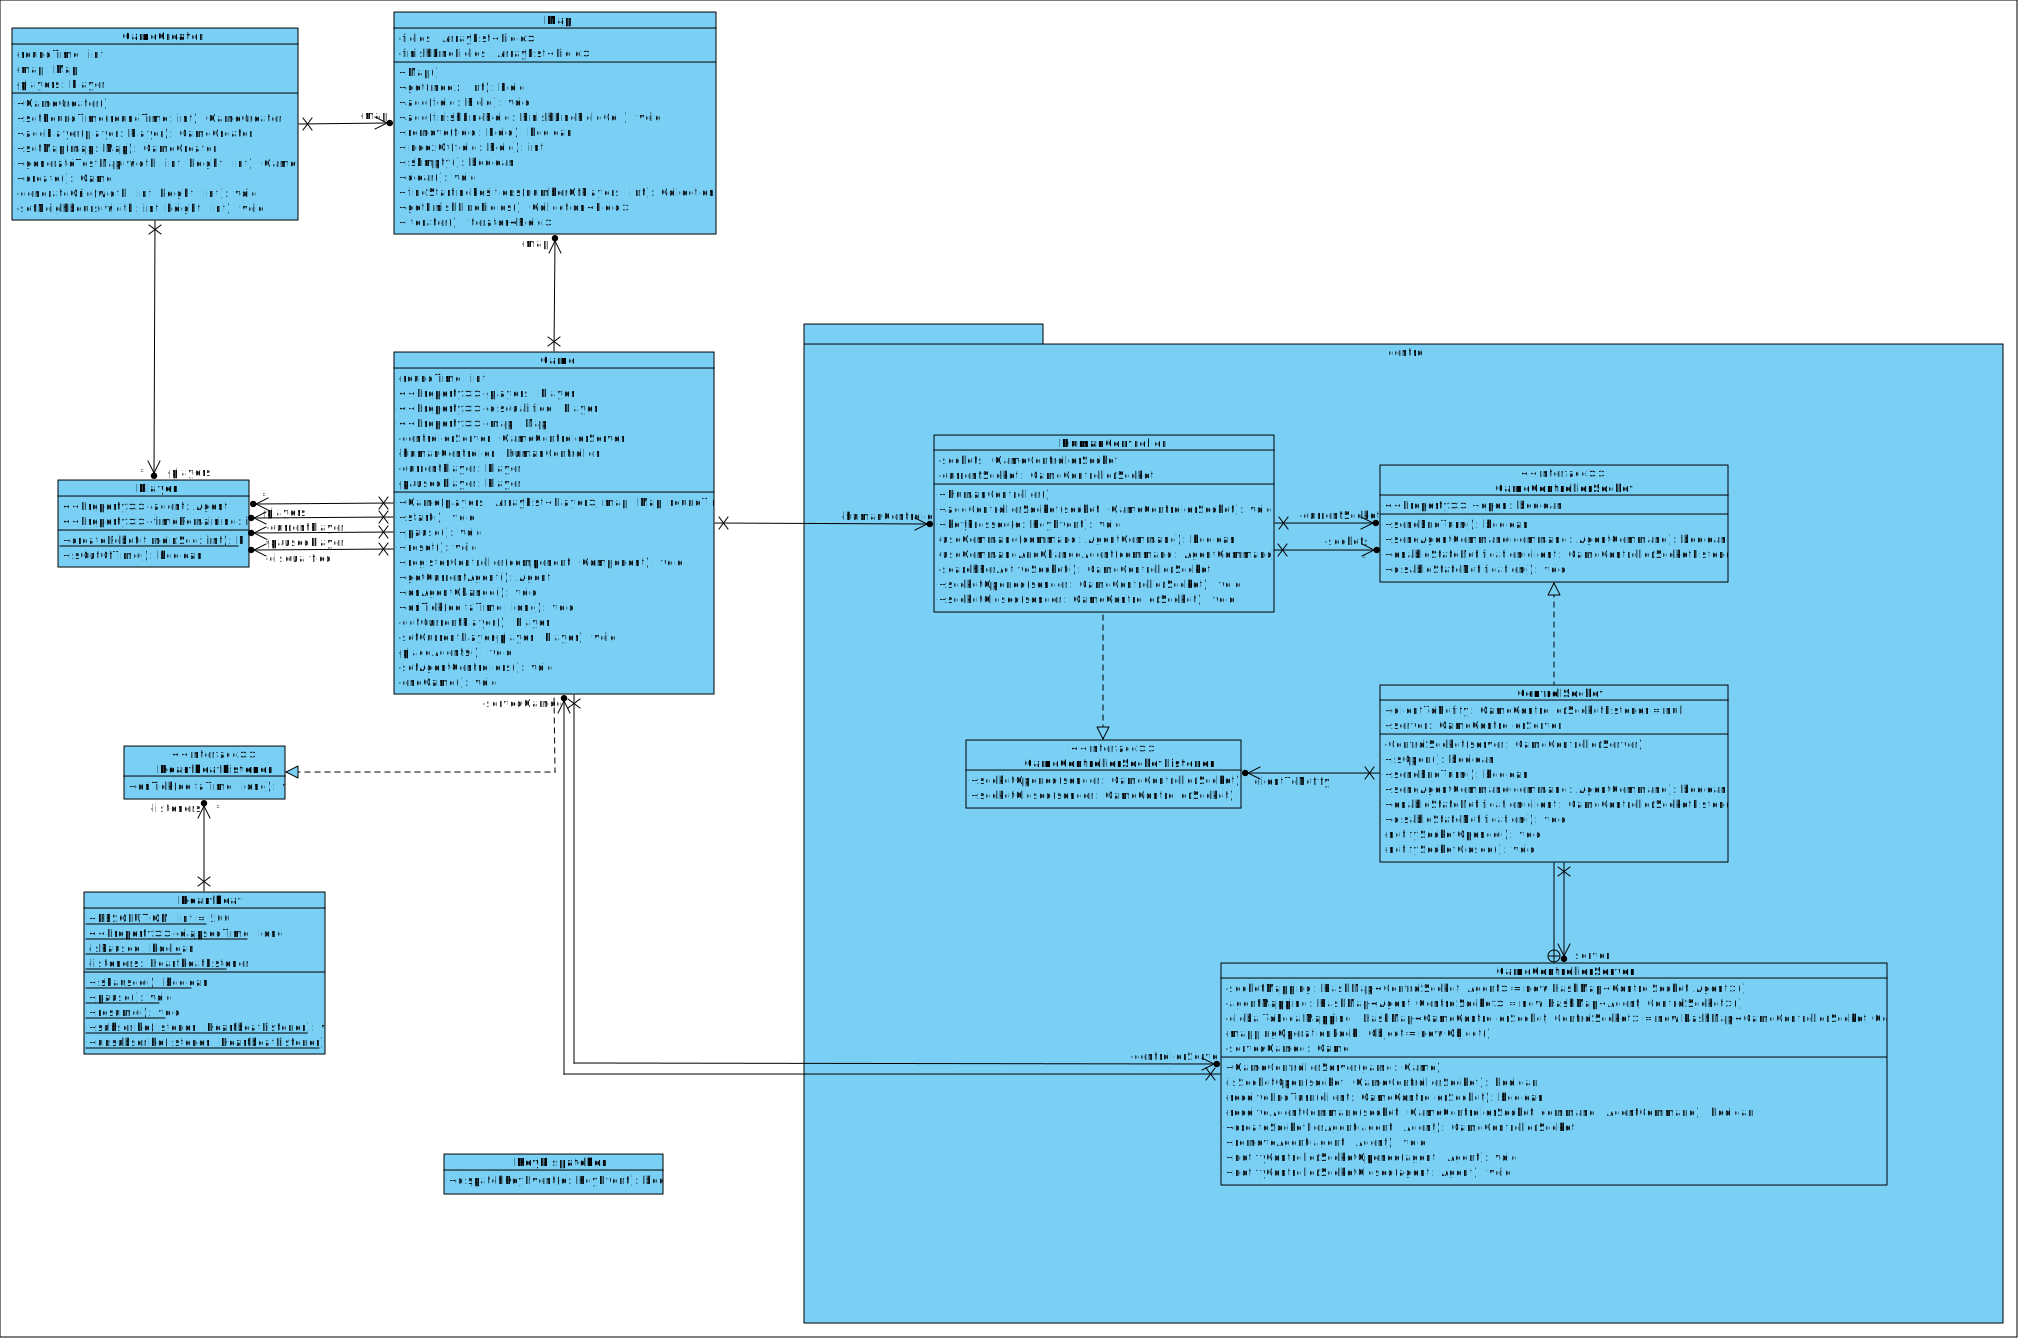
\includegraphics[width=\linewidth]{chapters/chapter07/gamepackage.pdf}
		\caption{Game package osztálydiagram}
		\label{Game package osztálydiagram}
	\end{center}
\end{figure}

\clearpage


\subsection{Szekvenciadiagram módosítások}
\begin{figure}[h]
	\begin{center}
		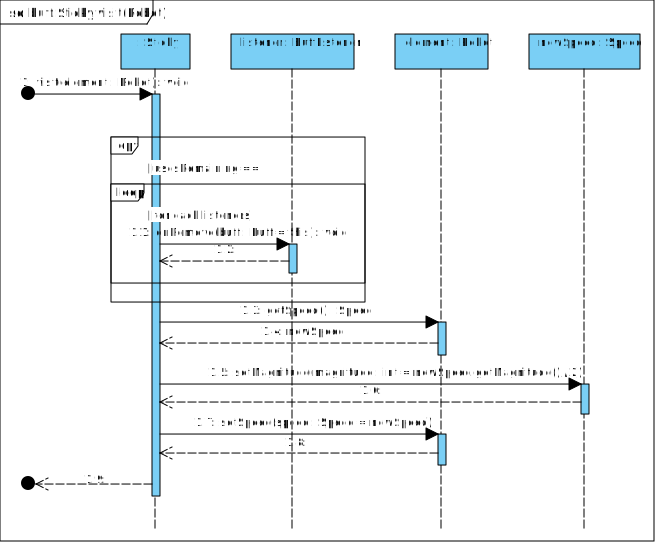
\includegraphics[width=\linewidth]{chapters/chapter07/ragacskopas.pdf}
		\caption{Ragacs kopása}
		\label{Ragacs kopása}
	\end{center}
\end{figure}

\clearpage

\begin{figure}[h]
	\begin{center}
		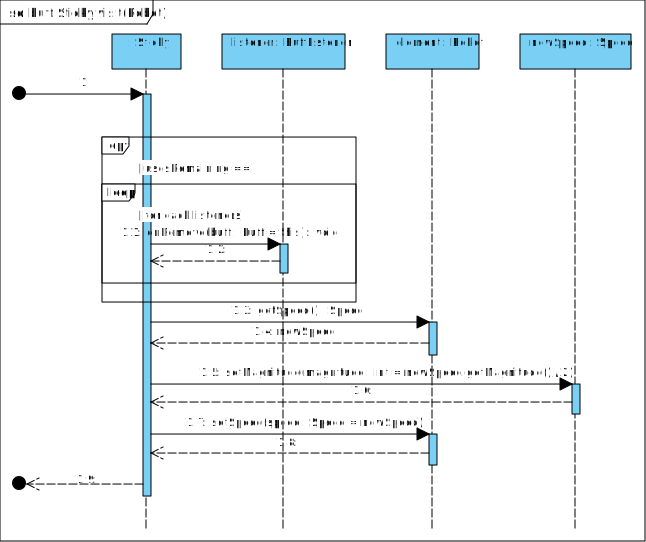
\includegraphics[width=\linewidth]{chapters/chapter07/olajszaradas.pdf}
		\caption{Olaj felszáradása}
		\label{Olaj felszáradása}
	\end{center}
\end{figure}

\clearpage

\begin{figure}[h]
	\begin{center}
		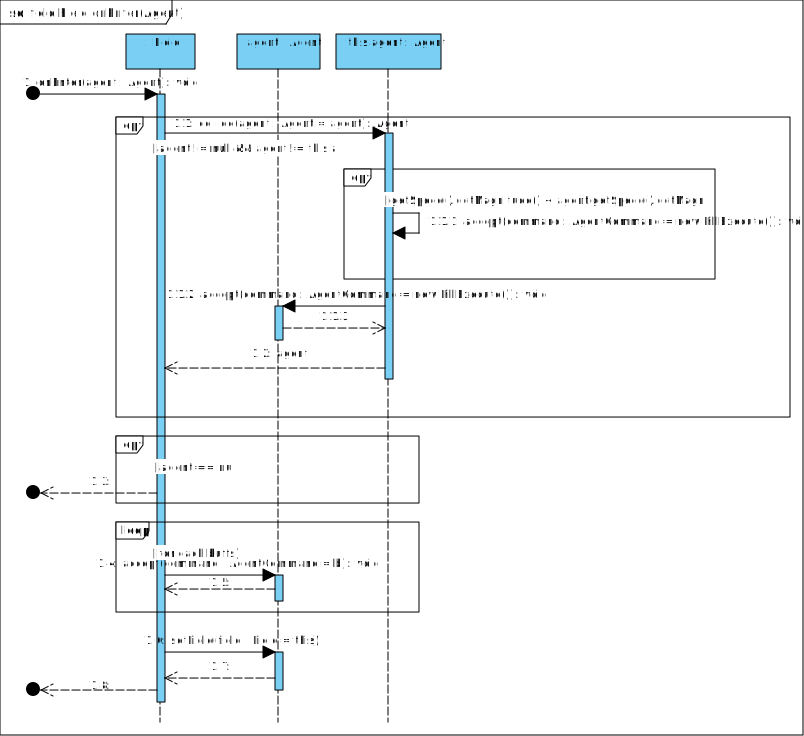
\includegraphics[width=\linewidth]{chapters/chapter07/utkozes.pdf}
		\caption{Robotok ütközése}
		\label{Robotok ütközése}
	\end{center}
\end{figure}

\clearpage


\section{Prototípus interface-definíciója}

\subsection{Az interfész általános leírása}
Az interfész a szabványos bemenetről tud fogadni parancsokat, a kimenetet pedig a szabványos kimenet jelenti. Ennek köszönhetően a használat
leegyszerűsödik, mivel a ki/bemenetek átirányításával lehetőség adódik ki/bemeneti fileokat megadni, melyek lehetőséget adnak a helyes működés
ellenőrzésére, amennyiben összehasonlításra kerülnek egy referenciakimenettel (mely az elvárt működést írja le.). Egy teszteset a prototípusnak
adható parancsok szekvenciájából, kimenet pedig az ezekre adott válaszokból áll. A tesztet sikeresnek mondhatjuk, ha a referenciakimenettel 
megegyező eredményt produkál. \\
A -rng kapcsolóval lehetőség adódik a randomizálható értékek generálására. Ezen kapcsoló hiányában a program tökéletesen determinisztikusan működik,
ez a funkció csak a tesztelői input rövidítésére szolgál. Viszont nem használható automata ellenőrzés esetén.\\
A -log kapcsoló lehetőséget ad a logok szintjének állítására például all/test/debug. \\

\subsection{Bemeneti nyelv}
A bemeneti nyelv az alábbi általános szintaxist használja: 

\lstset{escapeinside=`', xleftmargin=10pt, frame=single, basicstyle=\ttfamily\footnotesize, language=sh}
\begin{lstlisting}
parancs(arg1=ertek1, arg2=ertek2, arg3=ertek3)
\end{lstlisting}

\noindent A parancs végét a sor vége jelzi. Bármely parancs tetszőleges számú szóközzel tagolható, de a kis- és nagybetűket megkülönböztetik: az előző példával így egyenértékű például:

\lstset{escapeinside=`', xleftmargin=10pt, frame=single, basicstyle=\ttfamily\footnotesize, language=sh}
\begin{lstlisting}
parancs (arg1 = ertek1,arg2 = ertek2,arg3 = ertek3)
\end{lstlisting}

\noindent De külöböző tőle:

\lstset{escapeinside=`', xleftmargin=10pt, frame=single, basicstyle=\ttfamily\footnotesize, language=sh}
\begin{lstlisting}
PARANCS(arg1=ertek1, arg2=ertek2, arg3=ertek3)
\end{lstlisting}

\begin{itemize}

    \item jatek(szam=n, ido=m, palya=nev.map)
	\begin{itemize}
	    \item Leírás: Új játék kezdésére használt parancs.
	    \item Opciók:
            \begin{itemize}
                \item szam: a játékosok száma (2-4)
                \item ido: az egy játékosra jutó köridő
                \item palya: a betöltendő pálya neve
            \end{itemize}
	\end{itemize}
    
    \item betolt(nev=allas.sav)
    \begin{itemize}
        \item Leírás: Egy mentett játékállás betöltése
        \item Opciók: 
            \begin{itemize}
                \item nev: a mentett játékallás neve
            \end{itemize}
    \end{itemize}
    
    \item ment(nev=allas.sav)
    \begin{itemize}
         \item Leírás: Az aktuális játékállás elmentése
         \item Opciók: 
             \begin{itemize}
                 \item nev: a mentett játékallás neve
             \end{itemize}
    \end{itemize}

    \item ugrik()
    \begin{itemize}
        \item Leírás: Az aktuálisan soron lévő ágenset utasítja ugrásra
        \item Opciók: 
    \end{itemize}
    
    \item irvalt(irany=IRANY)
    \begin{itemize}
        \item Leírás: Az aktuálisan soron lévő ágens sebességének irányát változtatja meg
        \item Opciók: 
            \begin{itemize}
                \item irany: az új irány (lehetséges értékek: FEL, LE, BAL, JOBB)
            \end{itemize}
    \end{itemize}
    
    \item sebvalt(delta=n)
    \begin{itemize}
        \item Leírás: Az aktuálisan soron lévő ágens sebességének nagyságát változtatja
        \item Opciók: 
            \begin{itemize}
                \item delta: A változtatás nagysága (a program felülírhatja a felhasználó döntését, amennyiben az kívül esik az általa várt tartományon) 
            \end{itemize}
    \end{itemize}

    \item olajlerak()
    \begin{itemize}
        \item Leírás: Az aktuálisan soron lévő ágenset utasítja egy olajfolt lehelyezésére
        \item Opciók: 
    \end{itemize}

    \item ragacslerak()
    \begin{itemize}
        \item Leírás: Az aktuálisan soron lévő ágenset utasítja egy ragacsfolt lehelyezésére
        \item Opciók: 
    \end{itemize}
    
    \item vacuumlerak(field=fieldid)
    \begin{itemize}
    	\item Leírás: Lerak egy adott field-re egy kisrobotot.
       	\item Opciók: 
            \begin{itemize}
                  	\item field: Az adott field fieldid-ja
            \end{itemize}	
    \end{itemize}
    
    \item robotlerak(field=fieldid)
    \begin{itemize}
    	\item Leírás: Lerak egy adott field-re egy robotot
    	\item Opciók: 
    	\begin{itemize}
    		\item field: Az adott field fieldid-ja
    	\end{itemize}	
    \end{itemize}      
    
    \item olajleptet(ido=s)
    \begin{itemize}
    	\item Leírás: Az olaj hátralévő idejéből levesz s időt.
    	\item Opciók: 
    	\begin{itemize}
    		\item ido: A levonásra váró idő szekundumban
    	\end{itemize}	
    \end{itemize}
    
    \item olajlerak(field=fieldid)
    \begin{itemize}
       	\item Leírás: Lerak egy adott field-re egy olajat
       	\item Opciók: 
       	\begin{itemize}
       		\item field: Az adott field fieldid-ja
       	\end{itemize}	
    \end{itemize}
    
    \item ragacslerak(field=fieldid)
    \begin{itemize}
    	\item Leírás: Lerak egy adott field-re egy ragacsot
    	\item Opciók: 
    	\begin{itemize}
    		\item field: Az adott field fieldid-ja
    	\end{itemize}	
    \end{itemize}    
    
    \item vacuumtakarit()
    \begin{itemize}
    	\item Leírás: Elkezd takarítani a cellán, amin épp van. Ha nincs a cellán olaj, akkor nem takarít.
    	\item Opciók: 
    \end{itemize}    

    

\end{itemize}

\noindent A pályaképet a Java beépített szerializációs formátumában tároljuk, erről részletes leírás az alábbi linken olvasható:\\
\url{http://docs.oracle.com/javase/7/docs/platform/serialization/spec/serialTOC.html}

\subsection{Kimeneti nyelv}

\begin{itemize}
	\item Irányváltoztatás
	\begin{itemize}
		\item Kimenet <sikeres \{0\} | sikertelen \{1\}>
		\begin{itemize}
				\item \{0\} Robot: <robotid> Új irány: <újirány>
				\item \{1\} Sikertelen irányváltoztatás (Robot: <robotid>)
		\end{itemize}
	\end{itemize}
	
	\item Sebesség változtatás
	\begin{itemize}
		\item Kimenet <sikeres \{0\} | sikertelen \{1\}>
		\begin{itemize}
			\item \{0\} Robot: <robotid> Új sebesség: <újsebesség>
			\item \{1\} Sikertelen sebesség változtatás (Robot: <robotid>)
		\end{itemize}
	\end{itemize}
	
	\item Ugrás
	\begin{itemize}
		\item Kimenet <sikeres \{0\} | sikertelen \{1\}>
		\begin{itemize}
			\item \{0\} Robotid: <robotid> Előző cella: <fieldid> Új cella: <fieldid>
			\item \{1\} Sikertelen ugrás (Robot: <robotid>)
		\end{itemize}
	\end{itemize}
	
	\item Olaj lerakása cellára
	\begin{itemize}
		\item Kimenet <sikeres \{0\} | sikertelen \{1\}>
		\begin{itemize}
			\item \{0\} Robot: <robotid>  Érintett cella: <fieldid>
			\item \{1\} Sikertelen olaj lerakás (Robot: <robotid>)
		\end{itemize}
	\end{itemize}
	
	\item Ragacs lerakása cellára
	\begin{itemize}
		\item Kimenet <sikeres \{0\} | sikertelen \{1\}>
		\begin{itemize}
			\item \{0\} Robot: <robotid>. Érintett cella: <fieldid>
			\item \{1\} Sikertelen ragacs lerakás (Robot: <robotid>)
		\end{itemize}
	\end{itemize}	
	
	\item Új játék kezdése
	\begin{itemize}
		\item Kimenet <sikeres \{0\} | sikertelen \{1\}>
		\begin{itemize}
			\item \{0\} Generált pálya: <Map> Generált robotok: <Robot>
			\item \{1\} Sikertelen mentés.
		\end{itemize}
	\end{itemize}
	
	
	\item Játék elmentése
	\begin{itemize}
		\item Kimenet <sikeres \{0\} | sikertelen \{1\}>
		\begin{itemize}
			\item \{0\} Sikeres mentés megadott elérési útvonalra. 
			\item \{1\} Sikertelen mentés.
		\end{itemize}
	\end{itemize}

	\item Játék betöltése
	\begin{itemize}
		\item Kimenet <sikeres \{0\} | sikertelen \{1\}>
		\begin{itemize}
			\item \{0\} Betöltött pálya: <Map> Betöltött robotok <Robot> 
			\item \{1\} Sikertelen betöltés.
		\end{itemize}
	\end{itemize}
	
\end{itemize}


\section{Összes részletes use-case}
%\comment{A use-case-eknek a részletezettsége feleljen meg a kezelői felületnek, azaz a felület elemeire kell hivatkozniuk.}
Alábbi táblázat minden use-case-hez külön-külön.

\usecase%
{Új játék indítása}%
{Elindíthatunk egy új játékot}%
{Játékos, Játék}%
{A játékosok számának megadása után a Játékos kezdeményezheti a játéknak az elindítását}

\usecase%
{Játékparaméterek megadása}%
{Új játék paramétereinek megadása}%
{Játék}%
{Játékosok megadhatják, hogy hányan vannak, milyen időkorláttal kívánnak játszani}

\usecase%
{Játék megnyerése}%
{Játék végső helyzete alapján győztes eldöntése}%
{Játékos, Játék}%
{Ha minden Játékosnak lejár akkor a megtett út alapján eldől, hogy ki a győztes}

\usecase%
{Játék elvesztése}%
{Játék végső helyzete alapján vesztesek eldöntése}%
{Játékos, Játék}%
{Ha minden Játékosnak lejár akkor a megtett út alapján eldől, hogy kik a vesztesek}

\usecase%
{Játék elmentése}
{A játék jelenlegi állásának fájl(ok)ba mentése}
{Játékos, Játék}
{A Játékos megadja az elérési utat és a Játék elmenti a játékot}

\usecase%
{Játék betöltése}
{A játék fájlból való betöltése}
{Játékos, Játék}
{A Játékos megadja az elérési utat és a Játék betölti a játékot}

\usecase%
{Logolás}
{A játékos meghatározza, hogy logoljon a program}
{Játékos, Játék}
{A Játékos beállítja a logolás mértékét a -log kapcsolóval}

\usecase%
{Randomizálás}
{A játékos meghatározza, hogy véletlenszerű értékekkel működjön a program}
{Játékos, Játék}
{A Játékos az -rng kapcsolóval tudja ezt állítani}


\section{Tesztelési terv}
%\comment{A tesztelési tervben definiálni kell, hogy a be- és kimeneti fájlok egybevetésével miként végezhető el a program tesztelése. Meg kell adni teszt forgatókönyveket. Az egyes teszteket elég informálisan, szabad szövegként leírni. Teszt-esetenként egy-öt mondatban. Minden teszthez meg kell adni, hogy mi a célja, a proto mely funkcionalitását, osztályait stb. teszteli. Az alábbi táblázat minden teszt-esethez külön-külön elkészítendő.}

Tesztelést egy összetett parancssorozat végrehajtásával fogjuk elvégezni. Egy általunk megtervezett paranccsorozatot készítünk a bemeneti nyelven melyet az "Az interfész általános leírása" részben leírt módon átadunk a programnak. Tartalmazni fogja a felsorolt tesztesetek minden elemét oly módon hogy azokkal vizsgálható legyen a helyes működésnek a menete az esetlegesen játék szabályait nem követő utasítások ellenében is. Valamint előre elkészül egy kimeneti nyelven megírt helyes végrehajtásra utaló kimenet melyet a program össze tud vetni az általa generált kimenettel. A felhasználó számára pedig mutatja az egyező és eltérő sorokat is. 

\teszteset{Új játék indítása}%
{Elindítunk egy új játékmenetet}%
{Meggyőződés arról, hogy a program képes a játékkörnyezetet kialakítani vagy betölteni a megadott paraméterek alapján}

\teszteset{Új játék paramétereinek megadása}%
{Beállíthatjuk milyen pályán kívánnak a felhasználók játszani és hányan.}%
{Megvizsgálni, hogy tényleg megfelelően tárolódtak-e el a megadott paraméterek mely az új játékmenet kialakításához kell}

\teszteset{Pálya betöltése}%
{Eltárolt pályának a betöltése a játékhoz}%
{Meggyőzödhetünk általa, hogy az elmentett pála betöltését a program el tudja-e megfelelően végezni}

\teszteset{Új táték indítása}%
{Elindítunk egy új játékmenetet}%
{Meggyőződés arról, hogy a program képes a játékkörnyezetet kialakítani vagy betölteni a megadott paraméterek alapján}

\teszteset{Robot sebességének változtatása}%
{Egy robot sebességét, mely az ugrásának a vektoriális elmozdulását adja, tudjuk így meghatározni}%
{A sebesség tényleges megválozásának kimutatása és meghatározása}

\teszteset{Robot utasítása olaj lehelyezésére}%
{Egy robotot utasíthatunk arra, hogy a pályán hagyjon ott egy olajfoltot, mellyel más játékosokat hátráltatni tud}%
{A lehelyezés elvégézésének a biztosítása}

\teszteset{Robot utasítása ragacs lehelyezésére}%
{Egy robotot utasíthatunk arra, hogy a pályán hagyjon ott egy ragacsfoltot, mellyel más játékosokat hátráltatni tud}%
{A lehelyezés elvégézésének a biztosítása}

\teszteset{Robot utasítása másik robotra való ráugrásra}%
{Egy robot ha egy olyan mezőre ugrik melyen már van Robot, akkor a megadott feltételek alapján a gyengébb haladhat tovább}%
{Vizsgálandó, hogy tényleg a megfelelő Robot esik-e ki ebben az állapotban}

\teszteset{Pályáról lelépő robotot elakaszt}%
{Amennyiben egy robot lelép a pálya határain kívülre, akkor ezzel kiesik a játékból, nem tud többet mozogni}%
{Az elakasztás megtörténtének megvizsgálása}

\teszteset{Robot utasítása ugrásra}%
{Egy robotot utasíthatunk arra, hogy ugorjon, ezzel mozgást végezve a pályán, mely szügséges ahhoz, hogy elérhesse a játék célját}%
{Az ugrás végrehajtásának megtörténtének és más robotokkal ez során végzett interakciók biztosítása}

\teszteset{Olajos mező sebességváltoztatást nem enged}%
{Egy robottal olajos mezőre lépve a robot azt az akadályoztatást szenvedi el, hogy nem változtathatja meg sebességét}%
{Ellenőrizni, hogy egy ilyen folttal rendelkező mezőn egy, a robotnak adott sebességváltoztatás utasítás nem kerül érvényre}

\teszteset{Ragacsos mező sebességet megfelez}%
{Egy robotal ragacsos mezőre lépve az robot azt az akadályoztatást szenvedi el, hogy sebessége megfeleződik}%
{Ellenőrizni, hogy egy ilyen folttal rendelkező mezőn egy a robotnak a sebessége valóban megfeleződik}

\teszteset{Takarító robot működésének ellenőrzése}%
{A pályán időnként megjelenő takarító robotok melyek a foltokat takarítják le a pályáról}%
{Cél hogy ellenőrizzük, hogy ezek a robotok valóban találnak-e koszos mezőt és azt letakarítják-e}

\section{Tesztelést támogató segéd- és fordítóprogramok specifikálása}
A csapat a tesztelést támogató progamot egy egyszerű különbségellenőrzőnek képzeli el, mely képes a kimenetet egy referenciafilelal összehasonlítva megmondani,
hogy az output melyik sorában van eltérés a várt kimenettől. Ennek segítségével lehetőség nyílik a hiba felderítésére és javítására. Bemenetei a program által adott
teszteset outputja és a referenciafile. Kimenete az eltérések. 


%% Szglab4
% ===========================================================================
%
\section{Napló}

\begin{naplo}
	
	\bejegyzes
	{2015.03.25. ~8.00}
	{2 óra}
    {Paral Nagy} 
	{Értekezlet: Elkészíti a Konzultációs jegyzőkönyvet és résztvesz az órán.\newline } 
	
	\bejegyzes
	{2015.03.26. ~21.00}
	{2 óra}
	{Paral \newline Nyári \newline Szőke \newline Nagy} 
	{Értekezlet.
		Döntés: Feladatok felosztása az feladatok hozzárendelése a megfelelő emberekhez. A részletek megbeszélése, tervezés, koncepciók átgondolása.\newline } 

	\bejegyzes
	{2015.03.27. ~18.00}
	{1 óra}
	{Nagy} 
	{Tevékenység: Elkészíti az Interface általános leírását és a Tesztelői program leírását\newline } 			
	
	\bejegyzes
	{2015.03.28. ~08.00}
	{2 óra}
	{Nyári} 
	{Tevékenység: Elkészíti a Tesztelői tervet.\newline }
	
	\bejegyzes
	{2015.03.28. ~18.00}
	{2 óra}
	{Paral \newline Nyári \newline Szőke \newline Nagy} 
	{Értekezlet.
		Döntés: Az elkészített vázlatok egyeztetése és általános megbeszélés a feladatak elkészüléséről.\newline } 

	\bejegyzes
	{2015.03.28. ~20.00}
	{3 óra}
	{Szőke} 
	{Tevékenység: Elkészíti az Összes részletes use-caset.\newline }	

    \bejegyzes
    {2015.03.28. ~18.00}
    {2 óra}
    {Paral} 
    {Tevékenység: Elkészíti a Bemeneti nyelvet.\newline } 

    \bejegyzes
    {2015.03.29. ~20.00}
    {1 óra}
    {Paral} 
    {Tevékenység: Reviewra szánt idő a pull-requestekre.\newline } 

    \bejegyzes
    {2015.03.29. ~20.00}
    {1 óra}
    {Nagy} 
    {Tevékenység: Reviewra szánt idő a pull-requestekre.\newline } 

    \bejegyzes
    {2015.03.29. ~20.00}
    {1 óra}
    {Nyári} 
    {Tevékenység: Reviewra szánt idő a pull-requestekre.\newline } 

    \bejegyzes
    {2015.03.29. ~20.00}
    {1 óra}
    {Szőke} 
    {Tevékenység: Reviewra szánt idő a pull-requestekre.\newline } 
    
	\bejegyzes
	{2015.03.29. ~20.00}
	{30 perc}
	{Nagy} 
	{Tevékenység: Napló elkészítése.\newline } 
	
\end{naplo}





%\setcounter{chapter}{7}
%% Szglab4
% ===========================================================================
%
\chapter{Részletes tervek}

\thispagestyle{fancy}

\section{Osztályok és metódusok tervei}

\subsection{Osztály1}
\begin{itemize}
\item Felelősség\newline
\comment{Mi az osztály felelőssége. Kb 1 bekezdés. Ha szükséges, akkor state-chart is.}
\item Ősosztályok\newline
\comment{Mely osztályokból származik (öröklési hierarchia)\newline
Legősebb osztály $\rightarrow$ Ősosztály2 $\rightarrow$ Ősosztály3...}
\item Interfészek\newline
\comment{Mely interfészeket valósítja meg.}
\item Attribútumok\newline
\comment{Milyen attribútumai vannak}
	\begin{itemize}
		\item attribútum1: attribútum jellemzése: mire való, láthatósága (UML jelöléssel), típusa
		\item attribútum2: attribútum jellemzése: mire való, láthatósága (UML jelöléssel), típusa
	\end{itemize}
\item Metódusok\newline
\comment{Milyen publikus, protected és privát  metódusokkal rendelkezik. Metódusonként precíz leírás, ha szükséges, activity diagram is  a metódusban megvalósítandó algoritmusról.}
	\begin{itemize}
		\item int foo(Osztály3 o1, Osztály4 o2): metódus leírása, láthatósága (UML jelöléssel)
		\item int bar(Osztály5 o1): metódus leírása, láthatósága (UML jelöléssel)
	\end{itemize}
\end{itemize}

\subsection{Osztály2}
\begin{itemize}
\item Felelősség\newline
\comment{Mi az osztály felelőssége. Kb 1 bekezdés. Ha szükséges, akkor state-chart is.}
\item Ősosztályok\newline
\comment{Mely osztályokból származik (öröklési hierarchia)\newline
Legősebb osztály $\rightarrow$ Ősosztály2 $\rightarrow$ Ősosztály3...}
\item Interfészek\newline
\comment{Mely interfészeket valósítja meg.}
\item Attribútumok\newline
\comment{Milyen attribútumai vannak}
	\begin{itemize}
		\item attribútum1: attribútum jellemzése: mire való, láthatósága (UML jelöléssel), típusa
		\item attribútum2: attribútum jellemzése: mire való, láthatósága (UML jelöléssel), típusa
	\end{itemize}
\item Metódusok\newline
\comment{Milyen publikus, protected és privát  metódusokkal rendelkezik. Metódusonként precíz leírás, ha szükséges, activity diagram is  a metódusban megvalósítandó algoritmusról.}
	\begin{itemize}
		\item int foo(Osztály3 o1, Osztály4 o2): metódus leírása, láthatósága (UML jelöléssel)
		\item int bar(Osztály5 o1): metódus leírása, láthatósága (UML jelöléssel)
	\end{itemize}
\end{itemize}

\section{A tesztek részletes tervei, leírásuk a teszt nyelvén}
[A tesztek részletes tervei alatt meg kell adni azokat a bemeneti adatsorozatokat, amelyekkel a program működése ellenőrizhető. Minden bemenő adatsorozathoz definiálni kell, hogy az adatsorozat végrehajtásától a program mely részeinek, funkcióinak ellenőrzését várjuk és konkrétan milyen eredményekre számítunk, ezek az eredmények hogyan vethetők össze a bemenetekkel.]

\subsection{Általános játék logika}
\begin{itemize}
	\item Leírás\newline
	\item Játék kezdése. Az ágensek sorban végigmenve irányváltoztatás és sebességváltoztatás. Az ágensek egszerre ugratása. Vacuum lerakása egy adott field-re.
	\item Bemenet\newline
		jatek(szam=2, ido=5, palya=test.map) \newline
		irvalt(irany=LEFT) \newline
		sebvalt(+1) \newline
		irvalt(irany=RIGHT) \newline
		sebvalt(-1) \newline
	\item Elvárt kimenet\newline
	\comment{a proto kimeneti nyelvén megadva (lásd előző anyag)}
\end{itemize}

\subsection{Olaj és Vacuum kapcsolata 1}
\begin{itemize}
	\item Leírás\newline
	\item Játék kezdése után olaj lerakása, majd vacuum lerakása. A teszt lényege, hogy lássuk a vacuum helyesen talál céljául olajat.
	\item Bemenet\newline
		jatek(szam=2, ido=5, palya=test.map) \newline
		olajlerak() \newline
		vacuumlerak(field = 1) \newline
		vacuumlep() \newline
	\item Elvárt kimenet\newline
	\comment{a proto kimeneti nyelvén megadva (lásd előző anyag)}
\end{itemize}

\subsection{Olaj és Vacuum kapcsolata 2}
\begin{itemize}
	\item Leírás\newline
	\item Játék kezdése után vacuum és olaj lerakása ugyanarra a cellára. Végül Vacuum utasítása takarításra.
		\item Bemenet\newline
		jatek(szam=2, ido=5, palya=test.map) \newline
		olajlerak(field = 1) \newline
		vacuumlerak(field = 1) \newline
		vacuumtakarit() \newline
		vacuumtakarit() \newline		
	\item Elvárt kimenet\newline
	\comment{a proto kimeneti nyelvén megadva (lásd előző anyag)}
\end{itemize}

\subsection{Olaj léptetése}
\begin{itemize}
	\item Leírás\newline
	\item Játék kezdése után olaj lerakása majd utasítása száradásra.
	\item Bemenet\newline
		jatek(szam=2, ido=5, palya=test.map) \newline
		olajlerak(field=1) \newline
		olajszarad(field=1, ido=2500) \newline
		olajszarad(field=1, ido=2500) \newline				
	\item Elvárt kimenet\newline
	\comment{a proto kimeneti nyelvén megadva (lásd előző anyag)}
\end{itemize}

\subsection{Ragacsra ráugrás és kopás}
\begin{itemize}
	\item Leírás\newline
	\item Játék kezdése után ragacs lerakása, majd két ágens egymás után ráugrik. Ragacs jelen esetben 2 ugrás után lekopik.
	\item Bemenet\newline
		jatek(szam=2, ido=5, palya=test.map) \newline
		ragacslerak(field=45) \newline
		robotathelyez(robot=1, field=44) \newline
		sebvalt(+1) \newline
		irvalt(BAL) \newline
		ugrik() \newline
		listinfos(field=45) \newline
		listinfos(robot=1) \newline
		robotathelyez(robot=2, field=46) \newline
		sebvalt(+1) \newline
		irvalt(JOBB) \newline
		ugrik() \newline
		listinfos(field=50) \newline		
		listinfos(robot=1) \newline		
	\item Elvárt kimenet\newline
	\comment{a proto kimeneti nyelvén megadva (lásd előző anyag)}
\end{itemize}

\subsection{Olajra ráugrás}
\begin{itemize}
	\item Leírás\newline
	\item Játék kezdése után olaj lerakása, majd egy ágens ráugrik és megpróbál sebességet változtatni. 
	\item Bemenet\newline	
		jatek(szam=2, ido=5, palya=test.map) \newline
		ragacslerak(field=45) \newline
		robotathelyez(robot=1, field=44) \newline
		sebvalt(+1) \newline
		irvalt(BAL) \newline
		ugrik() \newline
		sebvalt(+1)	\newline
	\item Elvárt kimenet\newline
	\comment{a proto kimeneti nyelvén megadva (lásd előző anyag)}
\end{itemize}

\subsection{Robot lehelyez buffot}
\begin{itemize}
	\item Leírás\newline
	\item Játék kezdése után utasítjuk az első számú ágenst egy buff lerakására.
	\item Bemenet\newline	
		jatek(szam=2, ido=5, palya=test.map) \newline
		robotathelyez(robot=1, field=44) \newline
		ragacslerak() \newline
		listinfos(field=44) \newline
	\item Elvárt kimenet\newline
	\comment{a proto kimeneti nyelvén megadva (lásd előző anyag)}
\end{itemize}

\subsection{Vacuum olaj felé léptetése}
\begin{itemize}
	\item Leírás\newline
	\item Játék kezdése után lerakunk egy olajat egy cellára, majd egy vacuumot a pályán valahova. Végül léptetjük a vacuumot.
	\item Bemenet\newline
		jatek(szam=2, ido=5, palya=test.map) \newline
		olajlerak(field=45) \newline
		vacuumlerak(field=52) \newline
		vacuumlep() \newline
	\item Elvárt kimenet\newline
	\comment{a proto kimeneti nyelvén megadva (lásd előző anyag)}
\end{itemize}

\subsection{Vacuum feltakarítja az olajat}
\begin{itemize}
	\item Leírás\newline
	\item Játék kezdése után lerakunk egy olajat egy cellára, majd egy vacuumot a pályán valahova. Végül léptetjük a vacuumot.
	\item Bemenet\newline
		jatek(szam=2, ido=5, palya=test.map) \newline
		olajlerak(field=45) \newline
		vacuumlerak(field=45) \newline
		vacuumtakarit() \newline
		vacuumtakarit() \newline
		listinfos(field=45) \newline
	\item Elvárt kimenet\newline
	\comment{a proto kimeneti nyelvén megadva (lásd előző anyag)}
\end{itemize}

\subsection{Robot ráugrik vacuumra}
\begin{itemize}
	\item Leírás\newline
	\item Robot és vacuum lehelyezése. Robot utasítása vacuumra ugrásra.
	\item Bemenet\newline
		jatek(szam=2, ido=5, palya=test.map) \newline
		robotathelyez(robot=1, field=45) \newline
		sebvalt(+1) \newline
		irvalt(BAL) \newline
		vacuumlerak(field=44) \newline
		urgik() \newline
		listinfos(field=44) \newline
		listinfos(robot=1) \newline
	\item Elvárt kimenet\newline
	\comment{a proto kimeneti nyelvén megadva (lásd előző anyag)}
\end{itemize}

\subsection{Vacuum találkozik vacuummal}
\begin{itemize}
	\item Leírás\newline
	\item Két vacuum és egy olaj lehelyézese. Az olajtól messzebb lévő vacuum léptetése, akinek útjában van a másik vacuum
	\item Bemenet\newline
		jatek(szam=2, ido=5, palya=test.map) \newline
		olajlerak(field=49) \newline
		vacuumlerak(field=45) \newline
		vacuumlerak(field=44) \newline
		vacuumlep(vacuum=2) \newline
		listinfos(vacuum=2) \newline
	\item Elvárt kimenet\newline
	\comment{a proto kimeneti nyelvén megadva (lásd előző anyag)}
\end{itemize}

\subsection{Robot ütközik robottal}
\begin{itemize}
	\item Leírás\newline
	\item Két robot lehelyezése egy sorba, egymás felé irányítás és ütközés megfigyelése. 45ös fielden találkozás
	\item Bemenet\newline
	jatek(szam=2, ido=5, palya=test.map) \newline
	robotathelyez(robot=1, field=43) \newline
	robotathelyez(robot=2, field=46) \newline	
	sebvalt(+2) \newline
	irvalt(JOBB) \newline
	sebvalt(+1) \newline
	irvalt(BAL) \newline
	urgik() \newline
	listallagents() \newline
	\item Elvárt kimenet\newline
	\comment{a proto kimeneti nyelvén megadva (lásd előző anyag)}
\end{itemize}

\section{A tesztelést támogató programok tervei}
\comment{A tesztadatok előállítására, a tesztek eredményeinek kiértékelésére szolgáló segédprogramok részletes terveit kell elkészíteni.}


%% Szglab4
% ===========================================================================
%
\section{Napló}

\begin{naplo}
	
	\bejegyzes
	{2015.04.01. ~20.00}
	{3 óra}
	{Paral \newline Nyári \newline Szőke \newline Nagy} 
	{Értekezlet.
		Döntés: Feladatok felosztása az feladatok hozzárendelése a megfelelő emberekhez. A részletek megbeszélése, tervezés, koncepciók átgondolása.\newline } 

	\bejegyzes
	{2015.04.01. ~23.00}
	{30 perc}
	{Nagy} 
	{Tevékenység: Felveszi a feladatokat.\newline } 			
	
	\bejegyzes
	{2015.04.02. ~20.00}
	{2 óra}
	{Nyári} 
	{Tevékenység: Elkészíti a Tesztek részletes tervei, leírásuk a teszt nyelvén.\newline }
	
	\bejegyzes
	{2015.04.03. ~18.00}
	{2 óra}
	{Paral} 
	{Tevékenység: Javítja a Tesztek részletes tervei, leírásuk a teszt nyelvén.\newline }
	
  \bejegyzes
	{2015.04.03. ~21.00}
	{3 óra}
	{Paral \newline Nyári \newline Szőke \newline Nagy} 
	{Értekezlet.
		Döntés: Az elkészített vázlatok egyeztetése és általános megbeszélés a feladatak elkészüléséről.\newline } 

	\bejegyzes
	{2015.04.04. ~20.00}
	{3 óra}
	{Szőke} 
	{Tevékenység: Elkészíti a Kimeneti-bemeneti nyelv módosításokat.\newline }	

	\bejegyzes
	{2015.04.05. ~20.00}
	{2 óra}
	{Nagy} 
	{Tevékenység: Átnézi és javítja a Kimeneti-bemeneti nyelv módosításokat.\newline }	

    \bejegyzes
    {2015.04.05. ~18.00}
    {4 óra}
    {Paral} 
    {Tevékenység: Elkészíti az Elsődleges teszteseteket .\newline } 
 
    \bejegyzes
    {2015.04.06. ~20.00}
    {4 óra}
    {Nyári} 
    {Tevékenység: Javítja az Elsődleges teszteseteket .\newline } 
       
    \bejegyzes
    {2015.04.06. ~16.00}
    {2 óra}
    {Szőke} 
    { Tevékenység: Osztályok és metódusok terveiből dolgozik.\newline }    

    \bejegyzes
    {2015.04.06. ~16.00}
    {2 óra}
    {Paral} 
    { Tevékenység: Osztályok és metódusok terveiből dolgozik.\newline }    
    
    \bejegyzes
    {2015.04.06. ~16.00}
    {1 óra}
    {Nagy} 
    { Tevékenység: Osztályok és metódusok terveiből dolgozik.\newline }    
    
    \bejegyzes
    {2015.04.06. ~16.00}
    {2 óra}
    {Nyári} 
    { Tevékenység: Osztályok és metódusok terveiből dolgozik.\newline }    
    
    \bejegyzes
    {2015.04.06. ~23.00}
    {1 óra}
    {Paral} 
    {Tevékenység: Reviewra szánt idő a pull-requestekre.\newline } 

    \bejegyzes
    {2015.04.06. ~23.00}
    {1 óra}
    {Nagy} 
    {Tevékenység: Reviewra szánt idő a pull-requestekre.\newline } 

    \bejegyzes
    {2015.04.06. ~23.00}
    {1 óra}
    {Nyári} 
    {Tevékenység: Reviewra szánt idő a pull-requestekre.\newline } 

    \bejegyzes
    {2015.04.06. ~23.00}
    {1 óra}
    {Szőke} 
    {Tevékenység: Reviewra szánt idő a pull-requestekre.\newline } 
    
	\bejegyzes
	{2015.04.07. ~01.00}
	{30 perc}
	{Nagy} 
	{Tevékenység: Napló elkészítése.\newline } 
	
\end{naplo}





%\setcounter{chapter}{9}
%% Szglab4
% ===========================================================================
%
\chapter{Prototípus beadása}

\thispagestyle{fancy}

\section{Fordítási és futtatási útmutató}
\comment{A feltöltött program fordításával és futtatásával kapcsolatos útmutatás. Ennek tartalmaznia kell leltárszerűen az egyes fájlok pontos nevét, méretét byte-ban, keletkezési idejét, valamint azt, hogy a fájlban mi került megvalósításra.}

\subsection{Fájllista}
\begin{tabularx}{\linewidth}{| l | l | l | X |}
\hline
\textbf{Fájl neve} & \textbf{Méret} & \textbf{Keletkezés ideje} & \textbf{Tartalom} \tabularnewline
\hline \hline
\endhead
\fajl
{src/main/agents/AgentElement.java}
{161 byte}
{2015.02.27~06:09~}
{Az AgentElement interfész deklarációját tartalmazza.}

\fajl
{src/main/agents/Agent.java}
{875 byte}
{2015.02.27~06:09~}
{Az Agent osztály implementációját tartalmazza.}

\fajl
{src/main/agents/AgentVisitor.java}
{126 byte}
{2015.02.27~06:09~}
{Az AgentVisitor interfész deklarációját tartalmazza.}

\fajl
{src/main/agents/Robot.java}
{1171 byte}
{2015.02.27~06:09~}
{A Robot osztály implementációját tartalmazza.}

\fajl
{src/main/agents/Speed.java}
{1087 byte}
{2015.02.27~06:09~}
{A Speed osztály implementációját tartalmazza.}

\fajl
{src/main/buff/Buff.java}
{1404 byte}
{2015.02.27~06:09~}
{A Buff osztály implementációját tartalmazza.}

\fajl
{src/main/buff/Inventory.java}
{450 byte}
{2015.02.27~06:09~}
{Az Inventory osztály implementációját tartalmazza.}

\fajl
{src/main/buff/Oil.java}
{375 byte}
{2015.02.27~06:09~}
{Az Oil osztály implementációját tartalmazza.}

\fajl
{src/main/buff/Sticky.java}
{374 byte}
{2015.02.27~06:09~}
{A Sticky osztály implementációját tartalmazza.}

\fajl
{src/main/commands/AgentCommand.java}
{383 byte}
{2015.02.27~06:09~}
{Az AgentCommand osztály implementációját tartalmazza.}

\fajl
{src/main/commands/AgentCommandVisitor.java}
{490 byte}
{2015.02.27~06:09~}
{Az AgentCommandVisitor interfész deklarációját tartalmazza.}

\fajl
{src/main/commands/Command.java}
{654 byte}
{2015.02.27~06:09~}
{A Command osztály implementációját tartalmazza.}

\fajl
{src/main/commands/executes/ChangeDirectionExecute.java}
{1206 byte}
{2015.02.27~06:09~}
{A ChangeDirectionExecute osztály implementációját tartalmazza.}

\fajl
{src/main/commands/executes/ChangeSpeedExecute.java}
{1243 byte}
{2015.02.27~06:09~}
{A ChangeSpeedExecute osztály implementációját tartalmazza.}

\fajl
{src/main/commands/executes/JumpExecute.java}
{1262 byte}
{2015.02.27~06:09~}
{A JumpExecute osztály implementációját tartalmazza.}

\fajl
{src/main/commands/executes/KillExecute.java}
{616 byte}
{2015.02.27~06:09~}
{A KillExecute osztály implementációját tartalmazza.}

\fajl
{src/main/commands/executes/UseOilExecute.java}
{1143 byte}
{2015.02.27~06:09~}
{Az UseOilExecute osztály implementációját tartalmazza.}

\fajl
{src/main/commands/executes/UseStickyExecute.java}
{1176 byte}
{2015.02.27~06:09~}
{Az UseStickyExecute osztály implementációját tartalmazza.}

\fajl
{src/main/commands/FieldCommand.java}
{382 byte}
{2015.02.27~06:09~}
{A FieldCommand osztály implementációját tartalmazza.}

\fajl
{src/main/commands/FieldCommandVisitor.java}
{340 byte}
{2015.02.27~06:09~}
{A FieldCommandVisitor interfész deklarációját tartalmazza.}

\fajl
{src/main/commands/NoAgentCommandException.java}
{77 byte}
{2015.02.27~06:09~}
{A NoAgentCommandException osztály implementációját tartalmazza.}

\fajl
{src/main/commands/NoFieldCommandException.java}
{78 byte}
{2015.02.27~06:09~}
{A NoFieldCommandException osztály implementációját tartalmazza.}

\fajl
{src/main/commands/queries/ChangeDirectionQuery.java}
{803 byte}
{2015.02.27~06:09~}
{A ChangeDirectionQuery osztály implementációját tartalmazza.}

\fajl
{src/main/commands/queries/ChangeSpeedQuery.java}
{789 byte}
{2015.02.27~06:09~}
{A ChangeSpeedQuery osztály implementációját tartalmazza.}

\fajl
{src/main/commands/queries/JumpQuery.java}
{727 byte}
{2015.02.27~06:09~}
{A JumpQuery osztály implementációját tartalmazza.}

\fajl
{src/main/commands/queries/UseOilQuery.java}
{686 byte}
{2015.02.27~06:09~}
{Az UseOilQuery osztály implementációját tartalmazza.}

\fajl
{src/main/commands/queries/UseStickyQuery.java}
{704 byte}
{2015.02.27~06:09~}
{Az UseStickyQuery osztály implementációját tartalmazza.}

\fajl
{src/main/commands/transmits/ChangeDirectionTransmit.java}
{1008 byte}
{2015.02.27~06:09~}
{A ChangeDirectionTransmit osztály implementációját tartalmazza.}

\fajl
{src/main/commands/transmits/ChangeSpeedTransmit.java}
{1011 byte}
{2015.02.27~06:09~}
{A ChangeSpeedTransmit osztály implementációját tartalmazza.}

\fajl
{src/main/commands/transmits/JumpTransmit.java}
{1324 byte}
{2015.02.27~06:09~}
{A JumpTransmit osztály implementációját tartalmazza.}

\fajl
{src/main/feedback/Feedback.java}
{100 byte}
{2015.02.27~06:09~}
{A Feedback interfész deklarációját tartalmazza.}

\fajl
{src/main/feedback/NoFeedbackException.java}
{74 byte}
{2015.02.27~06:09~}
{A NoFeedbackException osztály implementációját tartalmazza.}

\fajl
{src/main/feedback/Result.java}
{554 byte}
{2015.02.27~06:09~}
{A Result osztály implementációját tartalmazza.}

\fajl
{src/main/field/Direction.java}
{80 byte}
{2015.02.27~06:09~}
{A Direction osztály implementációját tartalmazza.}

\fajl
{src/main/field/Displacement.java}
{335 byte}
{2015.02.27~06:09~}
{A Displacement osztály implementációját tartalmazza.}

\fajl
{src/main/field/EmptyFieldCell.java}
{952 byte}
{2015.02.27~06:09~}
{Az EmptyFieldCell osztály implementációját tartalmazza.}

\fajl
{src/main/field/FieldCell.java}
{630 byte}
{2015.02.27~06:09~}
{A FieldCell osztály implementációját tartalmazza.}

\fajl
{src/main/field/FieldElement.java}
{160 byte}
{2015.02.27~06:09~}
{A FieldElement interfész deklarációját tartalmazza.}

\fajl
{src/main/field/Field.java}
{1655 byte}
{2015.02.27~06:09~}
{A Field osztály implementációját tartalmazza.}

\fajl
{src/main/field/FieldVisitor.java}
{216 byte}
{2015.02.27~06:09~}
{A FieldVisitor interfész deklarációját tartalmazza.}

\fajl
{src/main/field/FinishLineFieldCell.java}
{614 byte}
{2015.02.27~06:09~}
{A FinishLineFieldCell osztály implementációját tartalmazza.}

\fajl
{src/main/game/AgentController.java}
{214 byte}
{2015.03.14~10:10~}
{Az AgentController osztály implementációját tartalmazza.}

\fajl
{src/main/game/ControllerListener.java}
{88 byte}
{2015.03.14~12:28~}
{A ControllerListener interfész deklarációját tartalmazza.}

\fajl
{src/main/game/GameCreator.java}
{2732 byte}
{2015.03.14~10:10~}
{A GameCreator osztály implementációját tartalmazza.}

\fajl
{src/main/game/Game.java}
{3291 byte}
{2015.03.14~10:10~}
{A Game osztály implementációját tartalmazza.}

\fajl
{src/main/game/HumanController.java}
{1887 byte}
{2015.03.14~10:10~}
{A HumanController osztály implementációját tartalmazza.}

\fajl
{src/main/game/KeyDispatcher.java}
{220 byte}
{2015.03.14~10:10~}
{A KeyDispatcher osztály implementációját tartalmazza.}

\fajl
{src/main/game/Map.java}
{1778 byte}
{2015.03.14~10:10~}
{A Map osztály implementációját tartalmazza.}

\fajl
{src/main/game/Player.java}
{660 byte}
{2015.03.14~10:10~}
{A Player osztály implementációját tartalmazza.}

\fajl
{src/main/Main.java}
{1367 byte}
{2015.02.12~23:16~}
{A Main osztály implementációját tartalmazza.}

\fajl
{src/test/TravisTester.java}
{162 byte}
{2015.02.13~00:27~}
{A TravisTester osztály implementációját tartalmazza.}

\end{tabularx}


\subsection{Fordítás}
\comment{A fenti listában szereplő forrásfájlokból milyen műveletekkel lehet a bináris, futtatható kódot előállítani. Az előállításhoz csak a 2. Követelmények c. dokumentumban leírt környezetet szabad előírni.}

\lstset{escapeinside=`', xleftmargin=10pt, frame=single, basicstyle=\ttfamily\footnotesize, language=sh}
\begin{lstlisting}
javac -d bin *.java
\end{lstlisting}

\subsection{Futtatás}
Az elkészült futtatható fájlok a build/install/softlab4/bin mappában találhatók. 
Ezeket parancssorból futtathatjuk:
\lstset{escapeinside=`', xleftmargin=10pt, frame=single, basicstyle=\ttfamily\footnotesize, language=sh}
\begin{lstlisting}
cd build
cd install
cd softlab4
cd bin
Windows: .\softlab4.bat 
Linux:   ./softlab4
\end{lstlisting}


\section{Tesztek jegyzőkönyvei}

\subsection{Teszteset1}
\comment{Az alábbi táblázatot az utolsó, sikeres tesztfuttatáshoz kell kitölteni}

\tesztok{...}{...}

\comment{Az alábbi táblázatot a megismételt (hibás) tesztek esetén kell kitölteni minden ismétléshez egyszer. Ha szükséges, akkor a valós kimenet is mellékelhető mint a teszt eredménye.}

\tesztfail{...}{...}{...}{...}{...}

\section{Értékelés}
\begin{ertekeles}
\tag{Paral} % Tag neve
{25}        % Munka szazalekban
\tag{Szőke}
{25}
\tag{Nyári}
{25}
\tag{Nagy}
{25}
\end{ertekeles}


%\section{Naplo}
\begin{naplo}

            {2015-04-07 08:00:00}
            {2 h}
            {Nagy}
            {Tevekenyseg: Konzultacio}

            {2015-04-07 08:00:00}
            {5 h}
            {Paral\newlineNyari\newlineNagy\newlineSzoke}
            {Ertekezlet: Altalanos megbeszeles az elorehaladsrol, tervezes.}

            {2015-04-09 17:00:00}
            {5 h}
            {Paral}
            {Tevékenység: Felkészíti a prototípus a parancsok kezelésére.}

            {2015-04-10 23:00:00}
            {5 h}
            {Nyari}
            {Tevékenység: Felkészíti a prototípust a tesztek lefuttatására.}

            {2015-04-11 22:00:00}
            {3 h}
            {Szoke}
            {Tevékenység: Ellenőrzi a prototípus képes-e lefuttatni a tesztek üzeneteit.}

            {2015-04-12 20:00:00}
            {3 h}
            {Nagy}
            {Tevékenység: Implementálja az ellenőrző programot.}

            {2015-04-13 17:00:00}
            {4 h}
            {Szoke}
            {Tevékenység: Kódot javít, implementálja a kimenetet.}

            {2015-04-14 18:00:00}
            {2 h}
            {Paral}
            {Tevékenység: Teszteket futtat.}

            {2015-04-15 19:00:00}
            {5 h}
            {Paral\newlineNyari\newlineNagy\newlineSzoke}
            {Ertekezlet: Altalanos megbeszeles az elorehaladsrol, tervezes.}

            {2015-04-17 17:00:00}
            {5 h}
            {Paral\newlineNyari\newlineNagy\newlineSzoke}
            {Ertekezlet: Altalanos megbeszeles az elorehaladsrol, tervezes.}

            {2015-04-18 17:00:00}
            {3 h}
            {Nyari}
            {Tevékenység: A korábbi megbeszélések javításait viszi bele a prototípusba és tesztel.}

            {2015-04-19 22:00:00}
            {2 h}
            {Szoke}
            {Tevékenység: Utolsó javításokat eszközöl és tesztel.}

            {2015-04-19 22:00:00}
            {1 h}
            {Paral}
            {Tevekenyseg: Reviewra szant ido.}

            {2015-04-19 22:00:00}
            {2 h}
            {Nagy}
            {Tevekenyseg: Reviewra szant ido.}

            {2015-04-19 22:00:00}
            {1 h}
            {Szoke}
            {Tevekenyseg: Reviewra szant ido.}

            {2015-04-19 22:00:00}
            {2 h}
            {Nyari}
            {Tevekenyseg: Reviewra szant ido.}
\end{naplo}


%\setcounter{chapter}{10}
%% Szglab4
% ===========================================================================
%
\chapter{Grafikus felület specifikációja}

\thispagestyle{fancy}

\section{A grafikus interfész}

\begin{figure}[h!]
\begin{center}
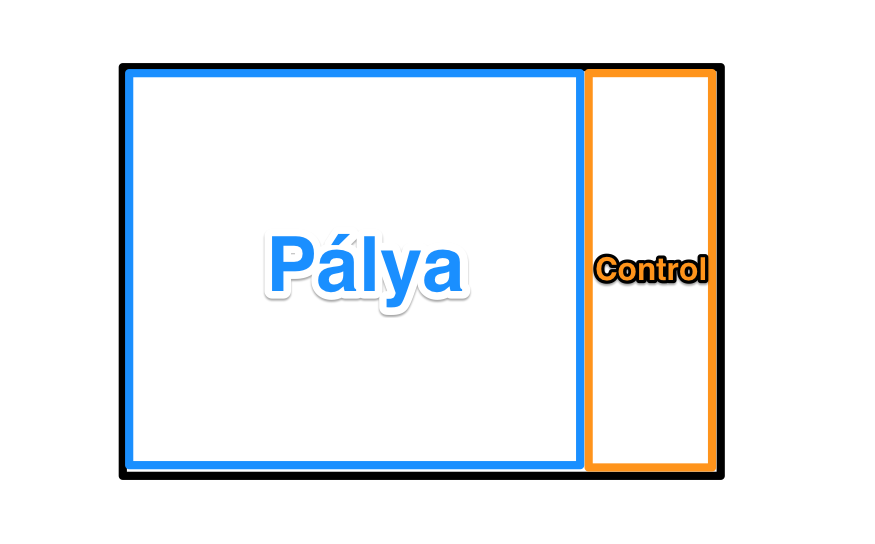
\includegraphics[width=17cm]{chapters/chapter11/1.png}
\caption{Panelek}
\label{fig:Grafikus}
\end{center}
\end{figure}

\begin{figure}[h!]
\begin{center}
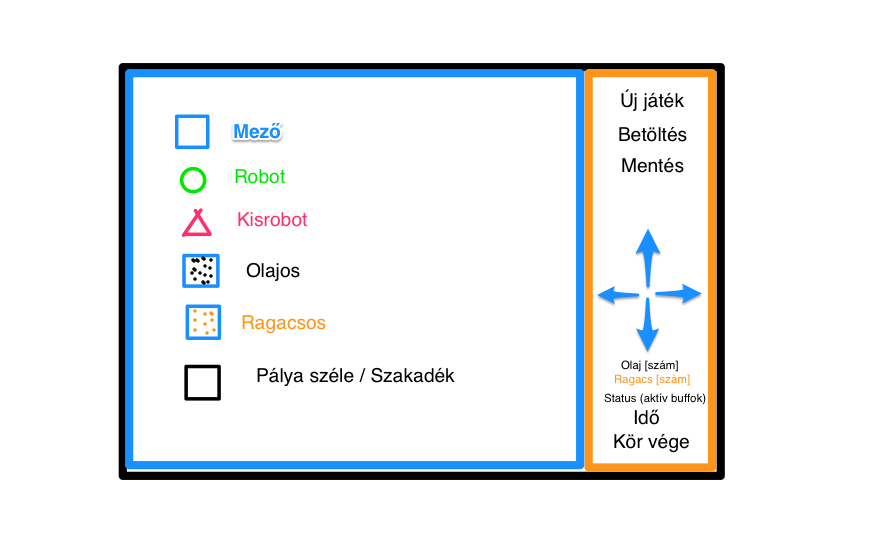
\includegraphics[width=17cm]{chapters/chapter11/2.png}
\caption{Lehetséges elemek a paneleken}
\label{fig:Grafikus}
\end{center}
\end{figure}

\begin{figure}[h!]
\begin{center}
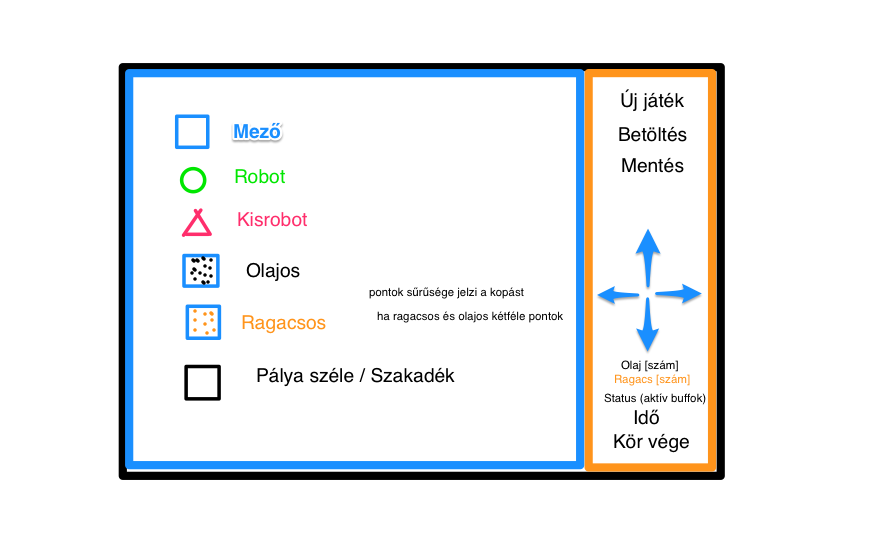
\includegraphics[width=17cm]{chapters/chapter11/3.png}
\caption{Magyarázatok}
\label{fig:Grafikus}
\end{center}
\end{figure}

\section{A grafikus rendszer architektúrája}
\comment{A felület működésének elve, a grafikus rendszer architektúrája (struktúra diagramok). A struktúra diagramokon a prototípus azon és csak azon osztályainak is szerepelnie kell, amelyekhez a grafikus felületet létrehozó osztályok kapcsolódnak.}

\subsection{A felület működési elve}
\noindent A grafikus felület \textbf{pull} alapú működést valósít meg, tehát mindig a felület megjelenítéséért felelős objektumok fogják lekérdezni a modell aktuális állapotát. 

\noindent Ezen új, a megjelenítést szolgáló objektumok adapterként szolgálnak a modell megfelelő elemeihez: minden megjeleníteni kívánt típushoz definiálni kell egy megjelenítőt (ezután: \textbf{Sprite}), ami képes visszaadni egy adott modellobjektum vizuális reprezentációját. 

\noindent A \textbf{Spriteokat} gyűjtőosztályok
foglalják magukba, amelyek létre tudják hozni a megfelelő \textbf{Spriteokat}, valamint képesek egy modellbeli absztrakt osztály vagy interfész (\textbf{Agent}, \textbf{Field} vagy \textbf{Buff}) grafikus reprezentációjának előállítására. 

\noindent A tényleges rajzolást egy osztály végzi, amely a képrenyőre rajzolja az összes, a gyűjtőosztályok által előállított képet.

\subsection{A felület osztály-struktúrája}
\comment{Osztálydiagram. Minden új osztály, és azon régiek, akik az újakhoz közvetlenül kapcsolódnak.}

\section{A grafikus objektumok felsorolása}

\subsection{AgentElementSprite}
\begin{itemize}
\item Felelősség \newline
    Az \textbf{Agent} absztrakt osztály leszármazott osztályainak grafikus reprezentációját állítja elő.
\item Ősosztályok
\item Interfészek
    \begin{itemize}
        \item AgentVisitor
        \item SpriteHandle
    \end{itemize}
\item Attribútumok
    \begin{itemize}
        \item -agent: Agent: az \textbf{Agent}, amelyikre az osztály vonatkozik
        \item -agentSprite: SpriteHandle: az \textbf{Agentnek} megfelelő \textbf{Sprite}
    \end{itemize}
\item Metódusok
	\begin{itemize}
        \item Agent getAgent(): visszaadja az osztály által kezelt \textbf{Agent} példányt
	\end{itemize}
\end{itemize}

\subsection{BuffElement}
\begin{itemize}
\item Felelősség \newline
    Ez az interfész előírja, hogy az őt implementáló osztályoknak képesnek kell lenniük \textbf{BuffVisitorok} fogadására. 
\item Ősosztályok
\item Interfészek
\item Attribútumok
\item Metódusok
	\begin{itemize}
        \item void accept(visitor: BuffVisitor): ez a metódus képes a \textbf{BuffVisitorok} fogadására
	\end{itemize}
\end{itemize}

\subsection{BuffElementSprite}
\begin{itemize}
\item Felelősség \newline
    A \textbf{Buff} absztrakt osztály leszármazott osztályainak grafikus reprezentációját állítja elő.
\item Ősosztályok
\item Interfészek
    \begin{itemize}
        \item BuffVisitor
        \item SpriteHandle
    \end{itemize}
\item Attribútumok
    \begin{itemize}
        \item -buff: Buff: a \textbf{Buff}, amelyikre az osztály vonatkozik
        \item -buffSprite: SpriteHandle: az \textbf{Buffnak} megfelelő \textbf{Sprite}
    \end{itemize}
\item Metódusok
	\begin{itemize}
        \item Buff getBuff(): visszaadja az osztály által kezelt \textbf{Buff} példányt
	\end{itemize}
\end{itemize}

\subsection{BuffVisitor}
\begin{itemize}
\item Felelősség \newline
    Ezen interfészt implementáló osztályok képessé válnak a \textbf{BuffElement} absztrakt osztály leszármazott osztályainak elérésére azoknak publikus interfészén keresztül.
\item Ősosztályok
\item Interfészek
\item Attribútumok
\item Metódusok
	\begin{itemize}
        \item void visit(element: Oil): egy \textbf{Oil} objektum elérésére képes annak publikus interfészén keresztül
        \item void visit(element: Sticky): egy \textbf{Sticky} objektum elérésére képes annak publikus interfészén keresztül
	\end{itemize}
\end{itemize}

\subsection{EmptyFieldCellSprite}
\begin{itemize}
\item Felelősség \newline
    Egy \textbf{EmptyFieldCell} grafikus reprezentációját állítja elő
\item Ősosztályok
\item Interfészek
    \begin{itemize}
        \item SpriteHandle
    \end{itemize}
\item Attribútumok
    \begin{itemize}
        \item -model: EmptyFieldCell: az osztály által kezelt \textbf{EmptyFieldCell}
        \item -image: BufferedImage (static): az osztály grafikus reprezentációját tartalmazó kép
    \end{itemize}
\item Metódusok
\end{itemize}

\subsection{FieldCellSprite}
\begin{itemize}
\item Felelősség \newline
    Egy \textbf{FieldCell} grafikus reprezentációját állítja elő
\item Ősosztályok
\item Interfészek
    \begin{itemize}
        \item SpriteHandle
    \end{itemize}
\item Attribútumok
    \begin{itemize}
        \item -model: FieldCell: az osztály által kezelt \textbf{FieldCell}
        \item -image: BufferedImage (static): az osztály grafikus reprezentációját tartalmazó kép
    \end{itemize}
\item Metódusok
\end{itemize}

\subsection{FieldElementSprite}
\begin{itemize}
\item Felelősség \newline
    A \textbf{Field} absztrakt osztály leszármazott osztályainak grafikus reprezentációját állítja elő.
\item Ősosztályok
\item Interfészek
    \begin{itemize}
        \item FieldVisitor
        \item SpriteHandle
    \end{itemize}
\item Attribútumok
    \begin{itemize}
        \item -field: Field: a \textbf{Field}, amelyikre az osztály vonatkozik
        \item -fieldSprite: SpriteHandle: az \textbf{Fieldnek} megfelelő \textbf{Sprite}
    \end{itemize}
\item Metódusok
	\begin{itemize}
        \item Field getField(): visszaadja az osztály által kezelt \textbf{Field} példányt
	\end{itemize}
\end{itemize}

\subsection{FinishLineFieldCellSprite}
\begin{itemize}
\item Felelősség \newline
    Egy \textbf{FinishLineFieldCell} grafikus reprezentációját állítja elő
\item Ősosztályok
\item Interfészek
    \begin{itemize}
        \item SpriteHandle
    \end{itemize}
\item Attribútumok
    \begin{itemize}
        \item -model: FinishLineFieldCell: az osztály által kezelt \textbf{FinishLineFieldCell}
        \item -image: BufferedImage (static): az osztály grafikus reprezentációját tartalmazó kép
    \end{itemize}
\item Metódusok
\end{itemize}

\subsection{GameGraphics}
\begin{itemize}
\item Felelősség \newline
    A \textbf{Spriteok} által előállított képek kirajzolása a képernyőre.
\item Ősosztályok
    \begin{itemize}
        \item jawax.swing.JPanel
    \end{itemize}
\item Interfészek
    \begin{itemize}
        \item jawa.awt.image.ImageObserver
    \end{itemize}
\item Attribútumok
    \begin{itemize}
        \item -bufferedImage: BufferedImage: a teljes kirajzolandó kép
        \item -map: game.Map: a kirajzolandó pálya
        \item -drawableFields: Map<Field, FieldElementSprite>: mapping a pálya \textbf{Fieldjei} és a grafikáért felelős \textbf{FieldElementSpriteok} között
    \end{itemize}
\item Metódusok
	\begin{itemize}
        \item bool attachToMap(map: game.Map): beállítja, hogy melyik pályát akarjuk kirajzolni
        \item void centerFieldTo(center: Field, radius: int): kirajzol egy NxM-es területet a megadott \textbf{Field} körül, ahol minden \textbf{Field} radius nagyságú
	\end{itemize}
\end{itemize}

\subsection{OilSprite}
\begin{itemize}
\item Felelősség \newline
    Egy \textbf{Oil} grafikus reprezentációját állítja elő
\item Ősosztályok
\item Interfészek
    \begin{itemize}
        \item SpriteHandle
    \end{itemize}
\item Attribútumok
    \begin{itemize}
        \item -model: Oil: az osztály által kezelt \textbf{Oil}
        \item -image: BufferedImage (static): az osztály grafikus reprezentációját tartalmazó kép
    \end{itemize}
\item Metódusok
\end{itemize}

\subsection{RobotSprite}
\begin{itemize}
\item Felelősség \newline
    Egy \textbf{Robot} grafikus reprezentációját állítja elő
\item Ősosztályok
\item Interfészek
    \begin{itemize}
        \item SpriteHandle
    \end{itemize}
\item Attribútumok
    \begin{itemize}
        \item -model: Robot: az osztály által kezelt \textbf{Robot}
        \item -startColorIndex: int (static): a \textbf{Robot} példányainak megkülönböztetésére használt statikus index
        \item -colorIndex: int: az aktuális \textbf{Robot} színének meghatározására használt index
    \end{itemize}
\item Metódusok
\end{itemize}

\subsection{SpriteHandle}
\begin{itemize}
\item Felelősség \newline
    Az interfészt implementáló osztályoknak elő kell tudniuk állitani saját grafikus reprezentációjukat
\item Ősosztályok
\item Interfészek
\item Attribútumok
\item Metódusok
	\begin{itemize}
        \item BufferedImage getItemImage(): visszaadja az implementáló osztály grafikus reprezentációját
	\end{itemize}
\end{itemize}

\subsection{StickySprite}
\begin{itemize}
\item Felelősség \newline
    Egy \textbf{Sticky} grafikus reprezentációját állítja elő
\item Ősosztályok
\item Interfészek
    \begin{itemize}
        \item SpriteHandle
    \end{itemize}
\item Attribútumok
    \begin{itemize}
        \item -model: Sticky: az osztály által kezelt \textbf{Sticky}
        \item -image: BufferedImage (static): az osztály grafikus reprezentációját tartalmazó kép
    \end{itemize}
\item Metódusok
\end{itemize}

\subsection{VacuumSprite}
\begin{itemize}
\item Felelősség \newline
    Egy \textbf{Vacuum} grafikus reprezentációját állítja elő
\item Ősosztályok
\item Interfészek
    \begin{itemize}
        \item SpriteHandle
    \end{itemize}
\item Attribútumok
    \begin{itemize}
        \item -model: Vacuum: az osztály által kezelt \textbf{Vacuum}
        \item -image: BufferedImage (static): az osztály grafikus reprezentációját tartalmazó kép
    \end{itemize}
\item Metódusok
\end{itemize}

\section{Kapcsolat az alkalmazói rendszerrel}
\comment{Szekvencia-diagramokon ábrázolni kell a grafikus rendszer működését. Konzisztens kell legyen az előző alfejezetekkel. Minden metódus, ami ott szerepel, fel kell tűnjön valamelyik szekvenciában. Minden metódusnak, ami szekvenciában szerepel, szereplnie kell a valamelyik osztálydiagramon.}


%\section{Naplo}
\begin{naplo}

            \bejegyzes
{2015-04-21 08:00:00}
            {2 h}
            {Paral\newline Nyari\newline}
            {Tevekenyseg: Konzultacio}
           

            \bejegyzes
{2015-04-21 08:00:00}
            {5 h}
            {Paral\newline Nyari\newline Nagy\newline Szoke}
            {Ertekezlet: Altalanos megbeszeles az elorehaladsrol, tervezes.}
           

            \bejegyzes
{2015-04-23 23:00:00}
            {5 h}
            {Paral\newline Nyari\newline Nagy\newline Szoke}
            {Ertekezlet: Altalanos megbeszeles az elorehaladsrol, tervezes.}
           

            \bejegyzes
{2015-04-24 21:00:00}
            {2 h}
            {Szoke}
            {Tevékenység: Kapcsolat az alkalmazói rendszerrel elkészítése.}
           

            \bejegyzes
{2015-04-25 17:00:00}
            {3 h}
            {Paral}
            {Tevékenység: A grafikus rendszer architektúrája}

            \bejegyzes
{2015-04-25 23:00:00}
            {3 h}
            {Nagy}
            {Tevékenység: A grafikus felület elkészítése}
           
            \bejegyzes
{2015-04-25 23:00:00}
            {4 h}
            {Paral}
            {Tevékenység: A grafikus felület elkészítése}
            
            \bejegyzes
{2015-04-25 23:00:00}
            {3 h}
            {Nyári}
            {Tevékenység: A felület működési elve}

            \bejegyzes
{2015-04-26 23:00:00}
            {1 h}
            {Paral}
            {Tevekenyseg: Reviewra szant ido.}
           

            \bejegyzes
{2015-04-26 23:00:00}
            {2 h}
            {Nagy}
            {Tevekenyseg: Reviewra szant ido.}
           

            \bejegyzes
{2015-04-26 23:00:00}
            {1 h}
            {Szoke}
            {Tevekenyseg: Reviewra szant ido.}
           

            \bejegyzes
{2015-04-26 23:00:00}
            {2 h}
            {Nyari}
            {Tevekenyseg: Reviewra szant ido.}
           
\end{naplo}


%\setcounter{chapter}{12}
%% Szglab4
% ===========================================================================
%
\chapter{Grafikus felület specifikációja}

\thispagestyle{fancy}

\section{Fordítási és futtatási útmutató}
\comment{A feltöltött program fordításával és futtatásával kapcsolatos útmutatás. Ennek tartalmaznia kell leltárszerűen az egyes fájlok pontos nevét, méretét byte-ban, keletkezési idejét, valamint azt, hogy a fájlban mi került megvalósításra.}

\subsection{Fájllista}

\begin{fajllista}

\fajl
{Main.java} % Kezdet
{250 byte} % Idptartam
{2009.10.10~18:05~} % Résztvevők
{...} % Leírás

\fajl
{...}
{...}
{...}
{...}

\end{fajllista}

\subsection{Fordítás}
\comment{A fenti listában szereplő forrásfájlokból milyen műveletekkel lehet a bináris, futtatható kódot előállítani. Az előállításhoz csak a 2. Követelmények c. dokumentumban leírt környezetet szabad előírni.}

\lstset{escapeinside=`', xleftmargin=10pt, frame=single, basicstyle=\ttfamily\footnotesize, language=sh}
\begin{lstlisting}
javac -d bin *.java
\end{lstlisting}

\subsection{Futtatás}
\comment{A futtatható kód elindításával kapcsolatos teendők leírása. Az indításhoz csak a 2. Követelmények c. dokumentumban leírt környezetet szabad előírni.}

\lstset{escapeinside=`', xleftmargin=10pt, frame=single, basicstyle=\ttfamily\footnotesize, language=sh}
\begin{lstlisting}
cd bin
java Main.java
\end{lstlisting}

\section{Értékelés}
\comment{A projekt kezdete óta az értékelésig eltelt időben tagokra bontva, százalékban.}

\begin{ertekeles}
\tag{Horváth} % Tag neve
{23.5}        % Munka szazalekban
\tag{Német}
{24.5}
\tag{Tóth}
{25}
\tag{Oláh}
{27}
\end{ertekeles}


%\section{Naplo}
\begin{naplo}

            \bejegyzes
            {2015-05-29 08:00:00}
            {2 h}
            {Paral\newline Nyari\newline Nagy\newline Szoke}
            {Tevekenyseg: Konzultacio}
           

            \bejegyzes
            {2015-05-29 08:00:00}
            {5 h}
            {Paral}
            {}
           

            \bejegyzes
            {2015-05-31 22:00:00}
            {5 h}
            {Nagy}
            {}
           

            \bejegyzes
            {2015-06-01 22:00:00}
            {1 h}
            {Paral\newline Nyari\newline Nagy\newline Szoke}
            {Ertekezlet: Altalanos megbeszeles az elorehaladsrol, tervezes.}
           

            \bejegyzes
            {2015-06-02 20:00:00}
            {2 h}
            {Paral}
            {}
           

            \bejegyzes
            {2015-06-03 20:00:00}
            {5 h}
            {Paral\newline Nyari\newline Nagy\newline Szoke}
            {Ertekezlet: Altalanos megbeszeles az elorehaladsrol, tervezes.}
           

            \bejegyzes
            {2015-06-04 20:00:00}
            {1 h}
            {Paral\newline Nyari\newline Nagy\newline Szoke}
            {Ertekezlet: Altalanos megbeszeles az elorehaladsrol, tervezes.}
           

            \bejegyzes
            {2015-06-05 21:00:00}
            {3 h}
            {Paral\newline Nyari\newline Nagy\newline Szoke}
            {Ertekezlet: Altalanos megbeszeles az elorehaladsrol, tervezes.}
           

            \bejegyzes
            {2015-06-06 22:00:00}
            {4 h}
            {Nyari}
            {}
           

            \bejegyzes
            {2015-06-07 18:00:00}
            {2 h}
            {Paral}
            {}
            
            \bejegyzes
            {2015-06-08 21:00:00}
            {1 h}
            {Nyari}
            {}

            \bejegyzes
            {2015-06-09 19:00:00}
            {1 h}
            {Paral\newline Nyari\newline Nagy\newline Szoke}
            {Ertekezlet: Altalanos megbeszeles az elorehaladsrol, tervezes.}

            \bejegyzes
            {2015-06-10 22:00:00}
            {2 h}
            {Paral\newline Nyari\newline Nagy\newline Szoke}
            {Ertekezlet: Altalanos megbeszeles az elorehaladsrol, tervezes.}

            \bejegyzes
            {2015-06-10 22:00:00}
            {1 h}
            {Paral}
            {Tevekenyseg: Reviewra szant ido.}
           

            \bejegyzes
            {2015-06-10 22:00:00}
            {2 h}
            {Nagy}
            {Tevekenyseg: Reviewra szant ido.}
           

            \bejegyzes
            {2015-06-10 22:00:00}
            {1 h}
            {Szoke}
            {Tevekenyseg: Reviewra szant ido.}
           

            \bejegyzes
            {2015-06-10 22:00:00}
            {2 h}
            {Nyari}
            {Tevekenyseg: Reviewra szant ido.}
           
\end{naplo}


%\setcounter{chapter}{13}
%% Szglab4
% ===========================================================================
%
\chapter{Összefoglalás}

\thispagestyle{fancy}

\section{Projekt összegzés}
\comment{A projekt tapasztalatait összegző részben a csapatoknak a projektről kialakult véleményét várjuk. A megválaszolandók köre az alábbi. }

\begin{munka}
\munkaido{Horváth}{98}
\munkaido{Németh}{95}
\munkaido{Tóth}{102}
\munkaido{Oláh}{87}
\osszesmunkaido{382}
\end{munka}

\begin{forrassor}
\munkaido{Szkeleton}{500}
\munkaido{Protó}{600}
\munkaido{Grafikus}{700}
\end{forrassor}

\begin{itemize}
\item Mit tanultak a projektből konkrétan és általában? \newline
\item Mi volt a legnehezebb és a legkönnyebb? \newline
\item Összhangban állt-e az idő és a pontszám az elvégzendő feladatokkal? \newline
\item Ha nem, akkor hol okozott ez nehézséget? \newline
\item Milyen változtatási javaslatuk van? \newline
\item Milyen feladatot ajánlanának a projektre? \newline
\end{itemize}

\comment{Szívesen fogadunk minden egyéb kritikát és javaslatot.}



\clearpage

% Függelék
%\appendix

\end{document}
